% ============================================================
% GPS Spoofing Detection for PX4-Based Unmanned Aerial Vehicles
% SIT724 / SIT746 Research Project — Deakin University
% Master file — compile with XeLaTeX
% ============================================================

\documentclass[12pt,a4paper]{report}

%%%----- PACKAGES -------------------------------------------
\usepackage{fontspec}
\usepackage[utf8]{inputenc}
\usepackage{geometry}
\geometry{a4paper, left=22mm, top=22mm, bottom=22mm, right=22mm}
\setlength{\headheight}{14.5pt}
\setlength{\headsep}{20pt}
\usepackage{setspace}
\usepackage{graphicx}
\graphicspath{{figures/}}
\usepackage{hyperref}
\usepackage{array}
\usepackage{booktabs}
\usepackage{longtable}
\usepackage{multirow}
\usepackage{amsmath}
\usepackage{amssymb}
\usepackage{enumitem}
\usepackage{caption}
\usepackage{subcaption}
\usepackage{xcolor}
\usepackage{fancyhdr}
\usepackage{listings}
\usepackage{tikz}
\usetikzlibrary{shapes,arrows,positioning,fit,backgrounds,calc}
\usepackage{algorithm}
\usepackage{algpseudocode}
\usepackage{float}

%%%----- FORMATTING -----------------------------------------
\renewcommand{\familydefault}{\sfdefault}
\hyphenpenalty=10000
\tolerance=10000
\onehalfspacing

%%%----- HYPERREF SETUP -------------------------------------
\hypersetup{
    colorlinks=true,
    linkcolor=blue,
    citecolor=blue,
    urlcolor=blue,
    pdftitle={GPS Spoofing Detection for PX4-Based Unmanned Aerial Vehicles},
    pdfauthor={Nikhil Sarwara},
}

%%%----- CODE LISTINGS STYLE --------------------------------
\lstset{
    basicstyle=\ttfamily\small,
    breaklines=true,
    frame=single,
    numbers=left,
    numberstyle=\tiny\color{gray},
    keywordstyle=\color{blue},
    commentstyle=\color{green!50!black},
    stringstyle=\color{orange},
    showstringspaces=false,
}

%%%----- HEADERS / FOOTERS ----------------------------------
\pagestyle{fancy}
\fancyhf{}
\fancyhead[L]{\rightmark}
\fancyhead[R]{\thepage}
\renewcommand{\headrulewidth}{0.4pt}

%------------- DOCUMENT BEGIN -------------------------------
\begin{document}

%========= TITLE PAGE =======================================
\thispagestyle{empty}
\begin{titlepage}
    \begin{center}
       \vspace*{1cm}
       % Deakin University Logo
       
\includegraphics[width=4cm]{deakin_logo.png}\\[0.5cm]
       {\large \textbf{DEAKIN UNIVERSITY}}\\[0.2cm]
       {\small Faculty of Science, Engineering and Built Environment}\\[1.5cm]

       {\LARGE \textbf{GPS Spoofing Detection for PX4-Based\\[0.3cm]
        Unmanned Aerial Vehicles}}\\[1.5cm]
       {\large A Software-Only Approach Using Sensor Fusion\\[0.2cm]
        and Machine Learning}\\[2cm]

        {\large Submitted as Research Report for\\[0.2cm]
         SIT746 Research Project (Advanced)}\\[1cm]

        {\large \textbf{Submission Date:} T1-2026}\\[0.5cm]
        {\large \textbf{May 2026}}\\[2cm]

        {\large \textbf{Nikhil Sarwara}}\\
        {\large Student ID: 224234862}\\
        {\large Master of Software Engineering (S464)}\\[1.5cm]

        {\normalsize Supervised by: Dr. Ananda Maiti}\\[1cm]

       \vfill
       {\normalsize Faculty of Science, Engineering and Built Environment}\\
       {\normalsize Deakin University}
    \end{center}
\end{titlepage}

%========= FRONT MATTER =====================================
\newpage
\thispagestyle{plain}
\pagenumbering{roman}
\setcounter{page}{1}

% ============================================================
% ABSTRACT
% ============================================================
\begin{abstract}
\noindent
Global Positioning System (GPS) spoofing poses a critical security threat to unmanned aerial vehicles (UAVs), as adversaries can transmit counterfeit signals to manipulate a drone's perceived position without triggering conventional failure modes. Existing countermeasures frequently depend on specialised hardware---multi-antenna arrays, military-grade encrypted signals, or high-grade inertial navigation systems---that are incompatible with the size, weight, and power constraints of commercial UAV platforms. This research presents a software-only GPS spoofing detection system for PX4-based drones that leverages cross-validation between GPS-reported position and inertial measurement unit (IMU) data to distinguish spoofing from environmental disturbances such as wind. The system employs a multi-layered detection pipeline combining eight physics-based heuristic rules with machine learning classifiers---Random Forest and one-dimensional Convolutional Neural Network---operating on 30-sample sliding windows of telemetry data acquired at 10\,Hz via the MAVLink protocol. Evaluated on a dataset of 4,207 telemetry records from 8 simulated flight runs in a PX4 Software-In-The-Loop environment with Gazebo, the Random Forest achieved 100\% accuracy on the held-out test set, while the 1D CNN exhibited perfect recall but a 100\% false positive rate on the limited normal-flight sample---a finding termed the ``CNN Paradox''. The key contribution is a physics-based GPS--IMU consistency discriminator that reliably identifies spoofing without requiring prior training on attack signatures. A graduated GPS Trust Index is proposed for real-time mitigation. The results demonstrate that real-time software-only spoofing detection is feasible, though the 3-second detection window exceeds theoretical safe-reaction times for high-speed scenarios, motivating future work on reduced-latency architectures and physical hardware validation.
\end{abstract}

\newpage
% ============================================================
% ACKNOWLEDGEMENTS
% ============================================================
\chapter*{Acknowledgements}
\addcontentsline{toc}{chapter}{Acknowledgements}

I would like to express my sincere gratitude to my supervisors for their invaluable guidance, constructive feedback, and continuous support throughout this research project. Their expertise in cyber-physical systems and embedded security has been instrumental in shaping the direction and quality of this work.

I am grateful to Deakin University and the Faculty of Science, Engineering and Built Environment for providing the resources, laboratory facilities, and academic environment that made this research possible.

Special thanks to my colleagues and peers for their thoughtful discussions, code reviews, and encouragement during the development of this system.

Finally, I wish to thank my family and friends for their unwavering patience, understanding, and support throughout my research journey. Their encouragement has been a constant source of motivation.

\newpage
% ============================================================
% LIST OF ABBREVIATIONS
% ============================================================
\chapter*{List of Abbreviations}
\addcontentsline{toc}{chapter}{List of Abbreviations}

\begin{tabular}{ll}
C/N$_0$  & Carrier-to-Noise Ratio \\
CNN      & Convolutional Neural Network \\
DEM      & Digital Elevation Model \\
DOI      & Digital Object Identifier \\
EKF2     & Extended Kalman Filter 2 \\
EMA      & Exponential Moving Average \\
ENU      & East-North-Up (coordinate system) \\
FPR      & False Positive Rate \\
GNSS     & Global Navigation Satellite System \\
GPS      & Global Positioning System \\
GTI      & GPS Trust Index \\
HDOP     & Horizontal Dilution of Precision \\
IMU      & Inertial Measurement Unit \\
INS      & Inertial Navigation System \\
MAVLink  & Micro Air Vehicle Link (communication protocol) \\
MEMS     & Micro-Electromechanical Systems \\
ML       & Machine Learning \\
MSL      & Mean Sea Level \\
OSNMA    & Open Service Navigation Message Authentication \\
PID      & Process Identifier \\
PVT      & Position, Velocity, and Time \\
PX4      & PX4 Autopilot (open-source flight stack) \\
RF       & Random Forest \\
RQ       & Research Question \\
RTL      & Return-to-Launch \\
SDF      & Simulation Description Format \\
SDR      & Software-Defined Radio \\
SITL     & Software-In-The-Loop \\
SWaP     & Size, Weight, and Power \\
TUI      & Terminal User Interface \\
UAV      & Unmanned Aerial Vehicle \\
UDP      & User Datagram Protocol \\
VDOP     & Vertical Dilution of Precision \\
\end{tabular}


%--------- TABLE OF CONTENTS --------------------------------
\newpage
\begin{singlespacing}
\tableofcontents
\end{singlespacing}

\newpage
\listoffigures
\listoftables

%========= MAIN BODY ========================================
\newpage
\pagenumbering{arabic}
\setcounter{page}{1}
\onehalfspacing

% ============================================================
% CHAPTER 1: INTRODUCTION
% ============================================================
\chapter{Introduction}

\section{Background and Motivation}

The proliferation of unmanned aerial vehicles (UAVs) across diverse operational domains---including civilian infrastructure inspection, precision agriculture, emergency response, environmental monitoring, and military reconnaissance---has elevated concerns regarding their vulnerability to Global Positioning System (GPS) spoofing attacks~\cite{Humphreys2012}. In such attacks, adversaries transmit counterfeit GPS signals synthesised with correct timing and structure but deliberately manipulated coordinates to usurp legitimate satellite navigation. The economic footprint of the commercial drone market is projected to reach \$54.6 billion by 2030, making the security of these platforms a matter of significant practical concern.

Unlike jamming, which merely attenuates or disrupts the GPS signal causing loss of lock, spoofing deceives the receiver into accepting falsified position, velocity, and time (PVT) estimates without any observable degradation in signal quality. Jamming denies service; spoofing corrupts service. A jamming attack is readily detected through carrier-to-noise ratio degradation. A spoofing attack, by contrast, is silent: the receiver continues to report a healthy fix while computing an incorrect but internally consistent PVT solution. The PX4 flight stack---which powers a substantial fraction of commercial and research drones worldwide---relies heavily on GPS as a primary input to its Extended Kalman Filter (EKF2) for state estimation~\cite{PX4Docs}. A successful spoofing attack can therefore cascade through the entire control pipeline, producing catastrophic trajectory deviations without triggering conventional failure modes~\cite{Kerns2014}.

The criticality of this threat was highlighted by a 2012 study in which researchers at the University of Texas successfully achieved full 3D control of a civilian UAV through GPS spoofing alone. In 2019, Iran claimed to have captured a US military drone by spoofing its GPS navigation. These incidents demonstrate that GPS spoofing is not a theoretical vulnerability but a practical, exploitable attack vector. Modern software-defined radios (SDRs) capable of generating counterfeit GPS signals are available for under \$300, dramatically lowering the barrier to entry for potential adversaries.

Existing countermeasures frequently depend on specialised hardware---multi-antenna arrays for angle-of-arrival discrimination, high-grade inertial navigation systems (INS) with tightly coupled integration, or military-grade encrypted signals (M-code, SAASM)---that are incompatible with the SWaP-constrained (Size, Weight, and Power) platforms that dominate the commercial UAV market. Cryptographic authentication schemes such as Galileo's Open Service Navigation Message Authentication (OSNMA) are promising but remain unavailable on the vast installed base of civilian receivers. A software-only detection mechanism that leverages sensors already present on standard PX4 autopilots represents a compelling and cost-effective alternative, provided it can achieve sufficient discriminative power in real time.

\section{Problem Statement}

The PX4 autopilot employs EKF2, a 24-state Extended Kalman Filter that fuses GPS, barometer, magnetometer, and IMU data to estimate position, velocity, attitude, and sensor biases. Under normal operation, EKF2 weights GPS position updates according to their reported accuracy (horizontal position error eph, vertical position error epv). When spoofed GPS data is injected, the EKF2 accepts the falsified position as a high-confidence observation because the spoofed signal reports low horizontal dilution of precision (HDOP) and healthy accuracy metrics.

The filter state is consequently dragged toward the attacker-controlled coordinates, while the IMU integration---which continues to reflect the drone's true physical motion---accumulates increasing innovation residuals relative to the corrupted GPS input. The EKF2's internal innovation monitoring will eventually reject GPS observations when the residual exceeds its configurable outlier gate. However, the latency of this natural rejection mechanism is unacceptably long for safety-critical flight operations. A dedicated anomaly detector that actively cross-validates GPS against IMU-derived motion estimates can flag spoofing before the EKF2 state is significantly corrupted.

The core research challenge is therefore: can we construct a practical, real-time GPS spoofing detector for commercial PX4 drones using only the sensors and telemetry already available, without requiring hardware modifications or firmware changes?

To make this vulnerability concrete, consider a simplified numerical scenario. A drone hovers at a true position of $(0, 0, 20)$\,m in the local ENU frame. At $t = 0$, a spoofing attack begins, injecting GPS positions that drift eastward at 2\,m/s. At $t = 1$\,s, the spoofed GPS reports $(0, 2, 20)$. The true drone position, as measured by the IMU, remains $(0, 0, 20)$---it has not physically moved. The EKF2 innovation (the difference between predicted position $(0, 0, 20)$ and observed position $(0, 2, 20)$) is 2\,m. With a typical PX4 innovation gate of 5--10\,m (configurable via the \texttt{EKF2\_GPS\_P\_GATE} parameter), the spoofed observation is accepted as valid. After 5 seconds, the drone's EKF2 state has been corrupted by 10\,m of eastward error, and the innovation has grown to 10\,m, potentially exceeding the gate. The drone has been flying on corrupted position estimates for 5 seconds---in that time, at 15\,m/s, it would have travelled 75\,m toward a potential obstacle. This numerical illustration demonstrates why a dedicated, rapid-responding spoofing detector is essential: the EKF2's natural protection mechanism is too slow for safety-critical flight.

\section{Research Questions}

This study is organised around three interdependent research questions:

\begin{enumerate}[label=\textbf{RQ\arabic*:},leftmargin=3em]
    \item \textbf{What are the primary vulnerabilities of GPS in autonomous mobile robots to spoofing attacks?} This question addresses the architectural and systemic weaknesses that enable spoofing to succeed, with specific focus on the PX4 flight stack.
    \item \textbf{How can sensor fusion techniques effectively detect GPS spoofing in real time?} This question operationalises the core insight that spoofing introduces a cross-sensor inconsistency between GPS-reported position and IMU-detected physical motion.
    \item \textbf{How can a dynamic GPS Trust Index be designed to quantify the reliability of GPS data?} This question extends detection from binary classification to continuous confidence metrics suitable for safety-critical operational decision-making.
\end{enumerate}

To evaluate RQ2 and RQ3, the following hypotheses guide the empirical analysis:

\begin{enumerate}[label=H\arabic*:,leftmargin=2em]
    \item GPS spoofing introduces measurable inconsistencies between GPS-reported position and inertial measurement unit (IMU) data that are distinguishable from normal flight disturbances.
    \item Physics-based heuristic rules can generate sufficiently accurate training labels without requiring laborious manual annotation of flight data.
    \item Machine learning classifiers---specifically Random Forest and one-dimensional Convolutional Neural Networks---can distinguish normal flight windows from spoofed segments using only standard PX4 telemetry.
    \item A live inference pipeline can process streaming MAVLink telemetry with latency suitable for real-time onboard detection.
\end{enumerate}

\section{Research Aims and Objectives}

The primary objectives of this research are:

\begin{enumerate}
    \item \textbf{Develop} a real-time GPS spoofing detection system for PX4-based drones using software-only techniques deployable on existing hardware without firmware modification.
    \item \textbf{Create} an automated labelling mechanism using eight physics-based heuristic rules that eliminates the need for manually annotated training data.
    \item \textbf{Train and evaluate} two complementary machine learning models---Random Forest and 1D Convolutional Neural Network---for accurate binary classification of GPS behaviour.
    \item \textbf{Design and implement} a comprehensive management interface integrating terminal-based component control with web-based monitoring and log visualisation.
    \item \textbf{Validate} the complete system through controlled simulated attack scenarios in a reproducible PX4 Software-In-The-Loop environment.
    \item \textbf{Propose} a graduated GPS Trust Index and post-detection response protocol for operational use.
\end{enumerate}

\section{Scope and Significance}

This research is scoped to PX4-based quadcopter platforms operating in the PX4 Software-In-The-Loop (SITL) simulation environment with Gazebo physics engine. The detection approach is exclusively software-based, leveraging standard telemetry data available on commercial PX4 autopilots without requiring hardware augmentation, firmware customisation, or access to encrypted GPS signals. The experimental scope covers 8 simulated flight runs with scripted rectangular survey patterns and controlled GPS spoofing injection via MAVLink GPS\_INPUT messages.

The significance of this work lies in demonstrating that cost-effective, real-time GPS spoofing detection is achievable using commodity sensor hardware and open-source software. By bridging the gap between theoretical academic demonstrations of GPS vulnerability and practical deployable countermeasures, this research contributes to the growing body of work on UAV cyber-physical security. The modular, open-source nature of the implementation enables reproducibility, extension, and adaptation to other autonomous platforms beyond the specific PX4 ecosystem.

To clarify the boundaries of this investigation, the following are explicitly out of scope: physical hardware flight tests (all validation is simulation-based), multi-drone swarm coordination scenarios, encrypted military GPS signal analysis, real-world radio-frequency spoofing from software-defined radio hardware, non-quadcopter platforms (fixed-wing, VTOL), and non-PX4 flight stacks (Ardupilot, BetaFlight). While these exclusions limit the immediate generalisability of findings, they define a focused, achievable scope appropriate for the resources and timeline of this research project.

\section{Thesis Structure}

The remainder of this thesis is organised as follows. \textbf{Chapter~2} reviews the relevant literature on GPS fundamentals, spoofing attack mechanisms, existing detection approaches from cryptographic, physical-layer, and sensor-fusion paradigms, PX4 architecture, and machine learning for anomaly detection. \textbf{Chapter~3} presents the high-level system design and architecture, including the key innovation of the GPS--IMU consistency discriminator. \textbf{Chapter~4} details the research methodology, simulation environment, data capture pipeline, preprocessing stages, heuristic labelling rules, model architectures, and evaluation metrics. \textbf{Chapter~5} describes the implementation of each system component with architectural detail and code-level documentation. \textbf{Chapter~6} presents the experimental results including dataset characterisation, model performance, the CNN Paradox analysis, live inference results, terrain-aware detection, and latency analysis. \textbf{Chapter~7} provides interpretation of findings, comparison with existing work, discussion of limitations and threats to validity, and the proposed GPS Trust Index with graduated response protocol. \textbf{Chapter~8} concludes the thesis with a summary of contributions, formal answers to each research question, practical implications, and directions for future work. Supplementary material is provided in the Appendix.

% ============================================================
% CHAPTER 2: LITERATURE REVIEW
% ============================================================
\chapter{Literature Review}

This chapter surveys the existing scholarly work relevant to GPS spoofing detection in unmanned aerial vehicles. The review is organised around six thematic areas: GPS fundamentals and vulnerabilities, spoofing attack mechanisms, existing detection approaches, PX4 flight stack architecture, sensor fusion techniques, and machine learning for anomaly detection. The chapter concludes by identifying specific research gaps that this work addresses.

\section{GPS Fundamentals and Vulnerabilities}

The Global Positioning System, a satellite-based radio-navigation system owned by the United States government and operated by the United States Space Force, provides geolocation and time information to GPS receivers anywhere on or near Earth~\cite{Shah2022}. The system architecture comprises three segments: the space segment, consisting of a nominal constellation of 31 satellites broadcasting on the L1 frequency (1575.42\,MHz) using Coarse/Acquisition (C/A) code and on the L2 frequency (1227.60\,MHz); the control segment, comprising a global network of ground stations that monitor satellite health, ephemeris, and clock corrections; and the user segment, consisting of commercial GPS receivers that compute PVT solutions from time-of-flight measurements to at least four satellites.

Civilian GPS employs the C/A code on L1, which is publicly documented in the GPS Interface Specification IS-GPS-200. While this openness has enabled widespread adoption across transportation, agriculture, telecommunications, and defence sectors, it creates inherent security vulnerabilities~\cite{Schmidt2021}. The signal structure is fully known, the navigation message is unauthenticated, and civilian receivers possess no mechanism to cryptographically verify the origin of received signals. This contrasts sharply with military GPS, which utilises encrypted Precision (P/Y) code and anti-spoofing modules that are inaccessible to civilian users.

GPS signals at the Earth's surface are extremely weak---approximately $-$130\,dBm, or below the thermal noise floor---making them susceptible to both intentional and unintentional interference. The low signal power enables a fundamental vulnerability: an adversary can generate a stronger, structurally valid counterfeit signal that overpowers the genuine satellite transmission, causing the receiver to track the spurious signal instead.

\section{GPS Spoofing: Threats and Attack Vectors}

\begin{figure}[H]
\centering
\begin{tikzpicture}[
    node distance=2.2cm and 1.8cm,
    block/.style={rectangle, draw, fill=blue!8, text width=2.8cm, text centered, minimum height=0.7cm, font=\small},
    bad/.style={rectangle, draw, fill=red!12, text width=2.8cm, text centered, minimum height=0.7cm, font=\small},
    arrow/.style={->, >=stealth, thick},
]
    \node[block] (sats) {GPS Satellites\\L1, 1575.42 MHz};
    \node[block, right=of sats] (rx) {Victim Receiver\\(PX4 + GPS)};
    \node[block, name=norm, below=of rx, yshift=-0.5cm] {Authenticated\\by IS-GPS-200};
    \node[block, below=of sats] (atk) {Attacker (SDR)\\Spoofing Signal};
    \node[bad, right=of atk, xshift=1cm] (cap) {PX4 accepts\\spoofed PVT};
    \node[bad, below=of cap] (drift) {Position drifts\\without IMU motion};

    \draw[arrow] (sats) -- (rx) node[midway,above] {Authentic};
    \draw[arrow] (atk.east) -- (cap.west) node[midway,above] {Counterfeit};
    \draw[arrow] (cap) -- (drift);
    \draw[arrow, dashed, gray] (rx.south) -- (norm.north);
\end{tikzpicture}
\caption{GPS spoofing attack flow: the attacker transmits a counterfeit signal structurally compliant with IS-GPS-200, causing the victim PX4 receiver to accept falsified PVT estimates while reporting a healthy fix.}
\label{fig:spoof_attack_flow}
\end{figure}

The cybersecurity literature often conflates two distinct categories of GPS interference: jamming and spoofing. Understanding their operational differences is critical for designing effective countermeasures.

\textbf{Jamming} broadcasts high-power noise in the GPS frequency band, elevating the noise floor until the receiver loses carrier-phase lock. Detection of jamming is straightforward: the receiver reports a precipitous drop in carrier-to-noise ratio (C/N$_0$) across all tracked satellites, followed by an explicit loss-of-fix status. Jamming is a denial-of-service attack; the receiver knows it has lost GPS.

\textbf{Spoofing}, in contrast, transmits a carefully constructed replica of authentic GPS signals with manipulated navigation data. Because the counterfeit signals comply with the IS-GPS-200 signal-in-space specification, the victim receiver synchronises to the attacker-generated signals, computes an incorrect but internally consistent PVT solution, and reports a healthy fix with normal C/N$_0$ and accuracy metrics~\cite{Zhang2020}. Spoofing is a corruption-of-service attack; the receiver believes it has accurate GPS.

Kerns et al.~\cite{Kerns2014} provided the first comprehensive open-source demonstration of civilian GPS spoofing using a low-cost software-defined radio platform, establishing that the threat is neither theoretical nor prohibitively expensive. Their work showed that a \$1,000 SDR could generate GPS signals that successfully captured a variety of commercial receivers. Humphreys~\cite{Humphreys2012} subsequently demonstrated full 3D control of a civilian unmanned aerial vehicle through GPS spoofing, raising significant policy and security concerns.

More recent research has explored increasingly sophisticated attack variants~\cite{Owen2019}:
\begin{itemize}
    \item \textbf{Slow-drift spoofing}: Gradually introducing position error at rates below typical detection thresholds (less than 0.5\,m/s), causing the EKF to slowly converge to the falsified position without triggering innovation monitoring.
    \item \textbf{Meaconing}: Recording and delayed rebroadcast of authentic GPS signals, which preserves the spatial consistency of the satellite geometry but introduces controlled temporal and positional offsets.
    \item \textbf{Multi-vehicle coordinated spoofing}: Simultaneously attacking multiple UAVs in a swarm with coordinated false positions that maintain inter-vehicle geometric consistency.
    \item \textbf{Carry-off attacks}: Starting with signals perfectly aligned to the authentic GPS and then smoothly increasing the divergence, making it difficult for the receiver to detect the transition.
\end{itemize}

\section{Existing Detection Approaches}

GPS spoofing detection has been approached through three broad paradigms: cryptographic authentication, physical-layer signal analysis, and sensor-fusion cross-validation.

\subsection{Cryptographic Authentication}

Cryptographic methods embed digital signatures or encryption in the GPS navigation message, enabling receivers to verify signal authenticity~\cite{Morales-Ferre2020}. Notable implementations include Galileo's Open Service Navigation Message Authentication (OSNMA), GPS Chimera, and the military M-code with Selective Availability Anti-Spoofing Module (SAASM). While cryptographically robust, these approaches require modifications to the satellite constellation, ground infrastructure, and receiver firmware. They are unavailable to the vast installed base of civilian receivers and cannot be retrofitted to existing PX4 flight controllers. Furthermore, cryptographic authentication cannot detect meaconing attacks where the signal itself is authentic but its timing has been manipulated.

\subsection{Physical-Layer Techniques}

Physical-layer methods exploit signal characteristics to discriminate authentic from counterfeit transmissions without cryptographic verification~\cite{Kumar2022}:
\begin{itemize}
    \item \textbf{Angle-of-Arrival (AOA) discrimination}: Comparing signal direction estimates across multiple antennas to detect spatially inconsistent signals from a single spoofing source.
    \item \textbf{Automatic Gain Control (AGC) monitoring}: Detecting the power increase associated with the introduction of a spoofing signal by monitoring receiver AGC levels.
    \item \textbf{Correlator output analysis}: Examining the distortion of the correlator peak shape that occurs when counterfeit and authentic signals overlap.
    \item \textbf{Vestigial signal detection}: Identifying residual authentic signals that remain visible below the stronger counterfeit signal.
\end{itemize}
These approaches require hardware augmentation---additional RF front-end components, multiple antennas, or modified receiver firmware---that is generally impractical for SWaP-constrained commercial UAV platforms.

\subsection{Sensor-Fusion Methods}

Sensor-fusion approaches leverage the physical inconsistency between GPS-reported motion and measurements from other onboard sensors~\cite{Broumandan2020}. The fundamental insight is that GPS spoofing affects only the position measurement domain, while inertial and environmental sensors remain faithful to true physical motion. This cross-sensor inconsistency is independent of the attacker's signal generation technique and cannot be concealed by improving the spoofing waveform fidelity.

Broumandan et al.~\cite{Broumandan2020} demonstrated that IMU-GPS inconsistency provides a robust spoofing indicator, particularly when integrated with INS-grade accelerometers and gyroscopes. Guizzaro et al.~\cite{Guizzaro2022} extended this work by applying neural network classifiers to IMU measurements for real-time spoofing detection. Manesh et al.~\cite{Manesh2019} developed a detection system specifically for UAV platforms using a combination of GPS signal metrics and machine learning.

The present work differs from these prior contributions in several important respects. First, we target standard low-cost PX4 hardware telemetry rather than navigation-grade IMUs. Second, we implement the cross-sensor check as both a standalone heuristic and an input feature to learned classifiers. Third, we integrate detection into a complete end-to-end pipeline with automated labelling, terrain-aware model selection, and graduated response protocols.

\section{PX4 Architecture and the EKF2}

The PX4 autopilot is an open-source flight control software stack widely adopted in both research and commercial UAV applications~\cite{PX4Docs}. Its state estimation system is built around EKF2, a 24-state Extended Kalman Filter that performs real-time sensor fusion with the following state vector components: position (3), velocity (3), attitude quaternion (4), delta-angle bias (3), delta-velocity bias (3), wind velocity (2), geomagnetic field (3), and magnetic field bias (3).

Under normal operation, EKF2 fuses observations from multiple sensor sources: GPS for absolute position and velocity, barometer for altitude, magnetometer for heading, and IMU for high-rate inertial propagation. Each observation is weighted according to its reported accuracy metrics. GPS observations are weighted by eph (horizontal position error) and epv (vertical position error). The innovation---the difference between the predicted measurement and the actual observation---is compared against a configurable threshold gate; observations exceeding this gate are rejected as outliers.

This architecture creates a specific vulnerability to GPS spoofing~\cite{Zhao2020}: because the spoofed signal artificially reports low eph/epv values, the EKF2 accepts the falsified position as a high-confidence observation. The filter state is progressively dragged toward the attacker-controlled coordinates, while IMU integration accumulates increasing innovation residuals. The natural EKF rejection mechanism triggers only when innovations have grown sufficiently large, which may require tens of seconds depending on the spoofing intensity and the specific gate configuration. During this period, the drone's control loops are acting on corrupted position estimates~\cite{Park2020}.

\begin{figure}[H]
\centering
\begin{tikzpicture}[
    node distance=1.5cm and 2cm,
    sensor/.style={rectangle, draw, fill=green!10, text width=2cm, text centered, minimum height=0.7cm, font=\small},
    ekf/.style={rectangle, draw, fill=blue!12, text width=2.5cm, text centered, minimum height=0.8cm, font=\small, rounded corners},
    outstyle/.style={rectangle, draw, fill=orange!10, text width=2cm, text centered, minimum height=0.7cm, font=\small},
    arrow/.style={->, >=stealth, thick},
]
    \node[sensor] (gps) {GPS\\Position, Vel};
    \node[sensor, below=of gps] (imu) {IMU\\Accel, Gyro};
    \node[sensor, below=of imu] (baro) {Barometer\\Altitude};
    \node[sensor, below=of baro] (mag) {Magnetometer\\Heading};
    \node[ekf, right=3cm of gps, yshift=-2.5cm] (ekf2) {EKF2\\24-State Filter\\Innovation Gating};
    \node[outstyle, right=of ekf2, xshift=1cm, yshift=1cm] (pos) {Position\\Estimate};
    \node[outstyle, right=of ekf2, xshift=1cm, yshift=-1cm] (vel) {Velocity\\Estimate};

    \draw[arrow] (gps.east) -- ++(1.5,0) |- (ekf2.north);
    \draw[arrow] (imu.east) -- ++(1.2,0) |- (ekf2.north west);
    \draw[arrow] (baro.east) -- ++(1.0,0) |- (ekf2.south west);
    \draw[arrow] (mag.east) -- ++(0.8,0) |- (ekf2.south);
    \draw[arrow] (ekf2.north east) -- ++(0.8,0) |- (pos.west);
    \draw[arrow] (ekf2.south east) -- ++(0.8,0) |- (vel.west);

    \node[font=\footnotesize, red, right=of gps, xshift=1.8cm, yshift=-0.5cm] {Spoofed input};
    \draw[->, red, thick] (gps.east) -- ++(0.5,0);
\end{tikzpicture}
\caption{PX4 EKF2 sensor fusion architecture. GPS, IMU, barometer, and magnetometer data feed into the 24-state Extended Kalman Filter. Under spoofing, the GPS input (highlighted in red) reports low error metrics, causing the EKF2 to weight it heavily despite containing falsified coordinates.}
\label{fig:ekf2_fusion}
\end{figure}

\section{Sensor Fusion for Anomaly Detection}

The theoretical foundation for the GPS--IMU consistency check is rooted in classical inertial navigation mechanics. An IMU contains three orthogonal accelerometers that measure specific force (acceleration plus gravitational component) and three orthogonal gyroscopes that measure angular rate~\cite{Kim2021}. The specific force vector, when resolved in the navigation frame, corrected for gravity, and double-integrated, yields position displacement. GPS provides absolute position measurements at lower update rates but with bounded long-term error.

Under normal flight dynamics, the displacement estimated from IMU integration and the displacement computed from GPS positions should agree within bounds determined by IMU noise characteristics, gravity modelling errors, and integration drift~\cite{Liu2021}. Wind gusts affect both sensor domains: GPS position changes because the vehicle is physically displaced, and IMU registers the corresponding acceleration and angular rates. GPS spoofing, however, introduces an asymmetry: GPS position changes without corresponding IMU-detected physical motion. This creates a measurable discrepancy in the cross-sensor consistency that is independent of the attacker's signal generation method.

The discriminative power of this inconsistency derives from fundamental physics rather than from assumptions about attack characteristics~\cite{Bhardwaj2019}. No spoofing technique---regardless of waveform fidelity, power level, or transition smoothness---can prevent the GPS-reported motion from diverging from the IMU-observed physical motion, because the attacker cannot physically manipulate the drone's inertia.

\subsection{EKF Innovation Monitoring and Rejection Latency}

The PX4 EKF2 includes built-in innovation monitoring that provides a natural, albeit slow, spoofing detection mechanism. Key diagnostic parameters streamed in the \texttt{ESTIMATOR\_STATUS} MAVLink message include: \texttt{vel\_innov} (velocity innovation), \texttt{pos\_horiz\_innov} (horizontal position innovation), and \texttt{pos\_vert\_innov} (vertical position innovation), each representing the Mahalanobis distance between the EKF-predicted measurement and the actual sensor observation. When an innovation value exceeds the configurable gate \texttt{EKF2\_GPS\_P\_GATE} (default: 5.0), the corresponding GPS observation is rejected, and the EKF propagates using IMU dead reckoning alone.

Under a typical spoofing attack with 2\,m/s position drift, the horizontal position innovation builds up at approximately 2\,m per second. With a default gate of 5.0, the innovation will exceed the gate after approximately 2.5 seconds. During this period, the EKF state estimate has already been corrupted by 5\,m of position error. The \texttt{GPS\_1\_PROTOCOL = 1} (MAVLink) parameter, required for the attack injector to function, further bypasses the receiver-level signal quality checks that would normally provide early warning. This EKF-level vulnerability directly motivates the companion detection system developed in this research, which aims to detect spoofing before the EKF innovation has grown large enough to trigger natural rejection.

\section{Machine Learning for Intrusion Detection}

The application of machine learning to GPS anomaly detection has gained significant attention in recent years. Two complementary model families have proven particularly effective for this domain.

\textbf{Random Forest classifiers} offer several advantages for GPS spoofing detection~\cite{Li2022}: they handle mixed feature types (continuous, categorical, binary) natively without extensive feature engineering; they are inherently robust to class imbalance through bootstrap aggregation and class weighting; they provide feature importance metrics that aid interpretability and model diagnostics; and they require minimal hyperparameter tuning compared to deep learning approaches. Random Forests have been successfully applied to GNSS spoofing detection by Guizzaro et al.~\cite{Guizzaro2022} and to broader UAV security tasks by Khan et al.~\cite{Khan2021}.

\textbf{One-dimensional Convolutional Neural Networks (1D CNNs)} are well-suited to multivariate time-series classification tasks such as GPS telemetry analysis~\cite{Zhang2023}. By applying convolutional filters along the temporal dimension, 1D CNNs can learn discriminative temporal patterns---such as the characteristic onset transient of a spoofing attack---without requiring manual feature extraction. Deep learning approaches for GNSS anomaly detection have been explored by Dang et al.~\cite{Dang2023} for cellular-connected UAV swarms and by Chen et al.~\cite{Chen2023} for autonomous drone navigation.

Key challenges confronting ML-based GPS spoofing detection include severe class imbalance (normal flight dominates operational data by orders of magnitude), temporal dependency (consecutive telemetry samples are not independent observations), concept drift (the characteristics of normal flight evolve with the operational environment), and the need for real-time inference on resource-constrained embedded platforms. The sliding window approach adopted in this thesis addresses temporal dependency; the automated heuristic labelling pipeline addresses the annotation bottleneck; and the terrain-aware model dispatching addresses environmental concept drift.

Table~\ref{tab:ml_comparison} summarises prior machine learning approaches to GNSS spoofing detection, providing a structured comparison with the present work.

\begin{table}[H]
\centering
\caption{Comparison of ML-based GNSS spoofing detection approaches.}
\label{tab:ml_comparison}
\small
\begin{tabular}{@{}lp{2.5cm}p{1.8cm}p{1.3cm}p{1.5cm}@{}}
\toprule
\textbf{Study} & \textbf{Sensors} & \textbf{Model} & \textbf{Real-Time} & \textbf{PX4 Compat.} \\
\midrule
Manesh et al.~\cite{Manesh2019} & GPS metrics only & MLP & No (offline) & No \\
Guizzaro et al.~\cite{Guizzaro2022} & IMU + GPS & Neural Net & Yes & No \\
Dang et al.~\cite{Dang2023} & GPS, cellular & GNN & Yes & No \\
Chen et al.~\cite{Chen2023} & GPS + vision & Deep NN & Yes & No \\
\textbf{This work} & \textbf{IMU + GPS + EKF} & \textbf{RF + CNN} & \textbf{Yes} & \textbf{Yes} \\
\bottomrule
\end{tabular}
\end{table}

The present work is distinguished from prior approaches by three characteristics: (a) explicit targeting of the PX4 ecosystem with compatibility verification, (b) use of EKF innovation metrics as features alongside raw sensor data, providing both physical and filter-level anomaly signals, and (c) a cascaded architecture where physics-based heuristics and learned classifiers complement each other, enabling detection before training data is available while improving discrimination as labelled data accumulates.

\section{Research Gaps}

A systematic survey of the literature reveals several specific gaps that this research addresses:

\begin{enumerate}
    \item \textbf{No existing software-only detector has been rigorously evaluated on PX4 platforms.} While prior work has demonstrated GPS spoofing detection using IMU cross-validation, these demonstrations either assumed navigation-grade sensors, required hardware modifications, or were evaluated in post-hoc offline analysis rather than real-time streaming inference.
    \item \textbf{The GPS--IMU consistency check has not been developed as a standalone, physics-based discriminator in a cascaded detection architecture.} Most sensor-fusion approaches treat IMU data as an additional feature channel for a learned classifier rather than leveraging it as a principled, model-free anomaly indicator.
    \item \textbf{The latency requirements for safety-critical UAV GPS spoofing detection have not been formally analysed.} While real-time detection is frequently cited as a requirement, no prior work has quantified the relationship between detection window length, inference latency, and available reaction time for obstacle avoidance.
    \item \textbf{No prior work has proposed a continuous GPS trust metric for graduated response.} Existing approaches typically produce binary detection outputs (spoofed / not spoofed), which are inadequate for safety-critical systems where the appropriate response may depend on the confidence of detection and the operational context.
    \item \textbf{Most detection systems require manually labelled training data, which is expensive and impractical to produce for the diverse range of attack types and environmental conditions.} An automated labelling pipeline using physics-based heuristics would significantly reduce the barrier to deployment.
\end{enumerate}

This research directly addresses these gaps by developing, implementing, and evaluating a complete GPS spoofing detection pipeline for PX4 UAVs that: (a) operates on standard telemetry without hardware augmentation; (b) employs a principled GPS--IMU consistency check as the core discriminator; (c) quantifies detection latency relative to safety constraints; (d) proposes a graduated GPS Trust Index for operational response; and (e) uses automated heuristic labelling to eliminate manual annotation requirements.

% ============================================================
% CHAPTER 3: SYSTEM DESIGN AND ARCHITECTURE
% ============================================================
\chapter{System Design and Architecture}

This chapter presents the high-level design and architecture of the GPS spoofing detection system. We discuss design requirements, the modular system architecture, individual component roles, and the key technical innovation---the GPS--IMU consistency discriminator.

\section{Design Requirements}

The system was designed to satisfy a set of functional and non-functional requirements derived from the research objectives and practical deployment constraints of the PX4 ecosystem.

\subsection{Functional Requirements}
\begin{enumerate}
    \item \textbf{F1---Telemetry Acquisition}: Collect GPS, IMU, and vehicle state data from a PX4 flight controller at a minimum rate of 10\,Hz via the MAVLink protocol~\cite{MAVLink}.
    \item \textbf{F2---Automated Labelling}: Automatically assign binary anomaly labels to each telemetry row using physics-based heuristic rules, eliminating the need for manual annotation.
    \item \textbf{F3---Data Processing Pipeline}: Transform raw CSV telemetry logs through a five-stage pipeline: cleaning, feature engineering, labelling, windowing, and dataset splitting.
    \item \textbf{F4---Model Training}: Train and serialise Random Forest and 1D Convolutional Neural Network classifiers from the labelled dataset~\cite{Pedregosa2011, Paszke2019}.
    \item \textbf{F5---Real-Time Inference}: Perform streaming anomaly detection on live MAVLink telemetry with sub-second latency and log results for review.
    \item \textbf{F6---Management Interface}: Provide both terminal-based component lifecycle management and web-based monitoring dashboard~\cite{StreamlitDocs}.
    \item \textbf{F7---Attack Simulation}: Generate controlled GPS spoofing attacks in a PX4 SITL environment for system testing and validation.
\end{enumerate}

\subsection{Non-Functional Requirements}
\begin{itemize}
    \item \textbf{Inference latency}: Less than 100\,ms for single-window prediction.
    \item \textbf{Detection accuracy}: Target above 85\% on balanced test sets.
    \item \textbf{Sampling consistency}: Maintain stable 10\,Hz logging without dropped messages during normal and spoofed flight segments.
    \item \textbf{Software-only deployment}: No hardware augmentation or firmware modifications required.
    \item \textbf{Modularity}: Each component (monitor, pipeline, inference, UI) runs independently and can be started/stopped without affecting others.
\end{itemize}

\section{Overall System Architecture}

The system follows a modular, pipeline-oriented architecture decomposed into eight logical subsystems following the ``divide and conquer'' decomposition principle. Figure~\ref{fig:system_arch} illustrates the overall architecture and data flow.

\begin{figure}[H]
\centering
\resizebox{\textwidth}{!}{
\begin{tikzpicture}[
    node distance=1.2cm,
    block/.style={rectangle, draw, fill=blue!10, text width=3cm, text centered, minimum height=0.8cm, rounded corners, font=\small},
    data/.style={rectangle, draw, fill=gray!15, text width=2.5cm, text centered, minimum height=0.7cm, font=\footnotesize},
    arrow/.style={->, >=stealth, thick},
]
    % Simulation
    \node[block] (px4) {PX4 SITL + Gazebo};
    \node[block, right=of px4] (mavlink) {MAVLink\\UDP Bridge};
    \node[block, right=of mavlink] (monitor) {GPS Monitor\\10 Hz Logger};
    \node[data, below=of monitor] (raw) {Raw CSVs};

    % Pipeline
    \node[block, right=of monitor, xshift=1.5cm] (clean) {Data\\Cleaning};
    \node[block, right=of clean] (label) {Auto-\\Labeling};
    \node[block, right=of label] (window) {Sliding\\Windows};
    \node[block, right=of window] (train) {Model\\Training};

    % Inference
    \node[block, below=of clean, yshift=-1.5cm] (infer) {Live Inference\\Engine};
    \node[block, right=of infer] (dashboard) {Streamlit\\Dashboard};
    \node[data, below=of infer] (log) {Inference Logs};

    % Attack
    \node[block, above=of px4] (attacker) {GPS Spoofer\\Attack Injector};

    % Arrows
    \draw[arrow] (px4) -- (mavlink);
    \draw[arrow] (mavlink) -- (monitor);
    \draw[arrow] (monitor) -- (raw);
    \draw[arrow] (raw.north) -- ++(0,0.3) -| (clean);
    \draw[arrow] (clean) -- (label);
    \draw[arrow] (label) -- (window);
    \draw[arrow] (window) -- (train);
    \draw[arrow] (train.south) -- ++(0,-0.3) -| (infer);
    \draw[arrow] (infer) -- (dashboard);
    \draw[arrow] (infer) -- (log);
    \draw[arrow] (attacker) -- (px4);

\end{tikzpicture}
}
\caption{System architecture showing data flow from PX4 simulation through GPS Monitor, ML Pipeline, and Live Inference to Dashboard. The attack injector provides controlled spoofing for testing.}
\label{fig:system_arch}
\end{figure}

The data flow proceeds as follows:
\begin{enumerate}
    \item PX4 SITL generates simulated flight physics and transmits telemetry via MAVLink over UDP port 14560.
    \item The GPS Monitor connects as a MAVLink client, captures 8 message types at 10\,Hz, and writes structured CSV logs.
    \item The ML Pipeline reads raw CSV files and sequentially executes data cleaning, automated labelling, sliding window creation, and model training.
    \item Trained models (RF and CNN) are serialised to disk for use by the inference engine.
    \item The Live Inference Engine consumes streaming MAVLink telemetry, accumulates 30-sample windows, and outputs anomaly probabilities with terrain-aware model selection.
    \item The Streamlit Dashboard displays live anomaly probabilities and a GPS Trust Index gauge, with historical log replay capability.
\end{enumerate}

\section{Component Overview}

The system comprises five major runtime components and one testing utility:

\begin{description}
    \item[GPS Monitor] pymavlink-based telemetry collector. Maintains a thread-safe state model of GPS, IMU, Estimator, and Vehicle Health data. Logs structured CSV at 10\,Hz with 34 fields per record. Includes a terminal-based real-time display with telemetry preview.
    \item[ML Pipeline] Python pipeline orchestrator supporting four processing modes: \texttt{process-single} (single flight), \texttt{process-batch} (all flights in directory), \texttt{train} (model training only), and \texttt{full} (end-to-end pipeline). Configuration-driven via YAML for reproducibility.
    \item[Live Inference Engine] Streaming detector with deque-buffered 30-sample sliding windows. Loads serialised models via joblib. Applies EMA smoothing for output stability. Supports terrain-aware model dispatching. Outputs labelled CSV log with per-window anomaly probability and metadata.
    \item[Streamlit Dashboard] Web interface with two operational modes: live monitor (GPS Trust Index gauge, telemetry display, anomaly probability chart) and log replay (upload and visualise historical inference logs). Auto-refreshes from the live log file.
    \item[TUI Management Console] Textual framework application providing component lifecycle management (start/stop with PID tracking), data file browser, ML pipeline execution buttons, integrated log viewer with colour-coded output, and one-click GPS spoofing attack launch.
    \item[GPS Spoofer] MAVLink GPS\_INPUT injector connecting as companion computer (sysid=1, compid=220). Supports six attack modes: drift, ramp drift, jump+drift, static freeze, teleport, and Gaussian noise. Includes warmup phase for EKF lock-in.
\end{description}

\section{Key Innovation: GPS--IMU Consistency Check}

The core technical innovation of this system is the physics-based GPS--IMU consistency discriminator, formally defined by Equation~\ref{eq:delta_phi_full} and implemented in practice via the heuristic indicator in Equation~\ref{eq:spoof_indicator}. This section presents the formal mathematical formulation and a worked example.

\subsection{Physical Principle}

The fundamental insight underpinning the consistency check is that natural flight disturbances---wind gusts, turbulence, pilot inputs---affect both GPS and IMU sensors simultaneously. A wind gust displaces the drone physically, which changes the GPS position and is registered by the accelerometers and gyroscopes. GPS spoofing, by contrast, changes the GPS position estimate without any corresponding physical motion: the IMU registers no acceleration or rotation because the drone is not actually moving.

\begin{figure}[H]
\centering
\begin{tikzpicture}[
    node distance=1.2cm,
    title/.style={font=\bfseries\small},
    sensor/.style={rectangle, draw, fill=gray!10, text width=2.8cm, text centered, minimum height=0.7cm, font=\small},
    agree/.style={font=\small\color{green!50!black}},
    disagree/.style={font=\small\color{red}},
    arrow/.style={->, >=stealth, thick},
]
    % Normal - wind
    \node[title] at (1.5, 0.5) {Normal Flight (Wind)};
    \node[sensor] (w1) at (0, 0) {GPS: Position\\Change Detected};
    \node[sensor] (w2) at (3.5, 0) {IMU: Acceleration\\Detected};
    \node[agree] at (1.75, -1) {Agree $\Rightarrow$ Normal};
    \draw[arrow] (w1.south) -- ++(0,-0.5) -| (1.75, -0.6);
    \draw[arrow] (w2.south) -- ++(0,-0.5) -| (1.75, -0.6);

    % Spoofed - no IMU
    \node[title] at (7.5, 0.5) {Spoofed Flight (No Wind)};
    \node[sensor] at (6, 0) (s1) {GPS: Position\\Change Detected};
    \node[sensor, fill=red!10] at (9.5, 0) (s2) {IMU: No Motion\\Detected};
    \node[disagree] at (7.75, -1) {Disagree $\Rightarrow$ ANOMALY};
    \draw[arrow] (s1.south) -- ++(0,-0.5) -| (7.75, -0.6);
    \draw[arrow] (s2.south) -- ++(0,-0.5) -| (7.75, -0.6);

    \draw[thick, gray, dashed] (5.2, -1.8) -- (5.2, 1);
\end{tikzpicture}
\caption{GPS--IMU consistency principle. Left: under a wind gust, both GPS and IMU detect the physical displacement---they agree. Right: under GPS spoofing, GPS reports position change while IMU registers no motion---the cross-sensor inconsistency reveals the attack.}
\label{fig:consistency_principle}
\end{figure}

This asymmetry creates a \textit{discriminative signal} that cannot be concealed by improving the spoofing waveform: regardless of how faithfully the counterfeit signal replicates authentic GPS structures, the discrepancy between GPS-reported and IMU-measured motion persists because the attacker cannot physically manipulate the drone's inertia.

\subsection{Mathematical Formulation}

Let \(\mathbf{P}_{\text{gps}, t} = (x_t, y_t, z_t)\) denote the GPS-reported position in local East-North-Up (ENU) Cartesian coordinates at time \(t\). Let \(\mathbf{a}_{\text{imu}}(t) \in \mathbb{R}^3\) denote the specific force vector measured by the IMU accelerometers, expressed in the navigation frame after gravity compensation.

The GPS--IMU consistency score over the time interval \([t_1, t_2]\) is defined as the Euclidean norm of the discrepancy between IMU-integrated displacement and GPS-reported displacement:

\begin{equation}
    \Delta \Phi(t_1, t_2) =
    \left\| \int_{t_1}^{t_2} \int_{t_1}^{\tau} \mathbf{a}_{\text{imu}}(s) \, ds \, d\tau
    \;-\; \bigl( \mathbf{P}_{\text{gps}, t_2} - \mathbf{P}_{\text{gps}, t_1} \bigr) \right\|_2
    \label{eq:delta_phi_full}
\end{equation}

The first term represents the displacement obtained by double-integrating the specific force measured by the IMU. The second term represents the displacement obtained by differencing two GPS position fixes. Under normal flight, these quantities should agree within a tolerance determined by IMU noise, gravity compensation errors, and integration drift~\cite{Hassan2023}. Under GPS spoofing, the second term reflects the attacker-controlled trajectory while the first term continues to reflect the drone's true motion.

For the heuristic implementation, this integral formulation is approximated using angular rate as a practical proxy for physical motion:

\begin{equation}
    \text{Spoofing Indicator} = \mathbb{I} \left[ \max_{i \in \{x,y,z\}} |\omega_i| < \tau_{\omega} \right]
    \;\cdot\; \mathbb{I} \left[ \| \mathbf{v}_{\text{gps}} \| > \tau_{v} \right]
    \label{eq:spoof_indicator}
\end{equation}

where \(\omega_i\) are the angular rates measured by the gyroscopes, \(\tau_{\omega} = 0.05\)\,rad/s is the quiescence threshold, and \(\tau_{v} = 5.0\)\,m/s is the GPS velocity threshold. The indicator is true only when the IMU is quiescent (no physical rotation) while GPS reports significant velocity---a condition that is physically impossible under authentic GPS but becomes true when spoofed positions are injected.

The empirical verification of this detector on the 8-flight simulation dataset, and its integration into a cascaded ML architecture, constitutes the primary experimental contribution of this research.

\subsection{Worked Numerical Example}

To make the GPS--IMU consistency principle concrete, consider two contrasting scenarios:

\textbf{Scenario A---GPS spoofing without wind.} A drone hovers at a fixed true position of $(0, 0, 20)$\,m in the local ENU frame. Over a 5-second interval, a spoofing attack injects GPS positions drifting eastward at 2\,m/s. At $t = 5$\,s, the spoofed GPS reports position $(0, 10, 20)$---a 10\,m eastward displacement. The IMU accelerometers, measuring the drone's true stationary state, register specific force near $(0, 0, 9.81)$\,m/s$^2$ (gravity only, no horizontal acceleration). Double-integrating yields IMU-estimated displacement $(0, 0, 0)$\,m. The GPS--IMU consistency score (Equation~\ref{eq:delta_phi_full}) evaluates to:

\[
\Delta \Phi = \| (0, 0, 0) - (0, 10, 0) \|_2 = 10\text{ m}
\]

which substantially exceeds the typical noise floor of the consistency score under normal flight (approximately 1--2\,m from IMU integration drift), correctly identifying the spoofing.

\textbf{Scenario B---Wind gust without spoofing.} The same drone experiences a 5\,m/s wind gust from the north at $t = 0$. The wind displaces the drone southward by 2\,m over 5 seconds: GPS reports $(0, -2, 20)$. The IMU registers the aerodynamic forces: horizontal acceleration of approximately 0.5\,m/s$^2$ from the induced body tilt (the quadcopter pitches to counteract drift). Double-integrating this acceleration yields IMU-estimated displacement approximately $(0, -1.8, 0)$\,m (the 0.2\,m discrepancy arises from IMU noise). The consistency score evaluates to:

\[
\Delta \Phi = \| (0, -1.8, 0) - (0, -2, 0) \|_2 = 0.2\text{ m}
\]

which is well within the typical 1--2\,m noise floor expected from IMU integration drift over a 5-second interval, correctly identifying the GPS data as authentic despite the environmental disturbance. This contrast illustrates the discriminative power of the consistency check: it distinguishes the asymmetric effect of spoofing (GPS moves, IMU does not) from the symmetric effect of wind (both sensors register the physical displacement).

% ============================================================
% CHAPTER 4: METHODOLOGY
% ============================================================
\chapter{Methodology}

This chapter presents the research methodology, experimental design, data collection procedures, preprocessing pipeline, heuristic labelling framework, machine learning model architectures, and evaluation strategy employed in this study.

\section{Research Methodology}

This research adopts a Design Science Research Methodology (DSRM) framework, which is well-suited to engineering research that produces both a functional artefact (the detection system) and theoretical contributions (the GPS--IMU consistency discriminator and the GPS Trust Index). The DSRM iterative cycle comprises: problem identification from literature and practice, solution design informed by identified gaps, artefact development through iterative implementation, evaluation via controlled experimentation, and theoretical generalisation of findings. Each cycle informs the subsequent iteration, with evaluation results driving refinements to both the detection algorithms and the system architecture.

\section{Simulation Environment}

A containerised Docker environment provides reproducible, scalable experimentation without risk to physical hardware. The simulation stack comprises:

\begin{itemize}
    \item \textbf{PX4 Software-In-The-Loop (SITL)}: The complete PX4 flight control firmware compiled for the host architecture, running identical control and estimation algorithms as physical hardware.
    \item \textbf{Gazebo Harmonic Physics Engine}: Simulates an Iris x500 quadcopter (3\,kg, 0.55\,m motor-to-motor) with realistic aerodynamics, rotor thrust curves, and configurable wind models.
    \item \textbf{QGroundControl / MAVSDK}: Ground control software for mission waypoint upload and telemetry visualisation.
    \item \textbf{MAVLink UDP Bridge}: Standard PX4 communication over \texttt{udp:127.0.0.1:14560}, with GPS Monitor connecting on port 14561.
\end{itemize}

The SITL approach enables controlled, repeatable attack scenarios under identical environmental conditions---a critical capability for evaluating detection algorithms where ground truth must be known with certainty.

\subsection{Gazebo Wind and Physics Models}

The PX4 SITL environment uses the Gazebo Harmonic physics engine to simulate vehicle dynamics. The Iris x500 quadcopter model is specified via an SDF (Simulation Description Format) file defining: mass (3\,kg), motor-to-motor diagonal distance (0.55\,m), rotor thrust curve (quadratic mapping from PWM to Newtons), aerodynamic drag coefficients, and moment of inertia tensor. These parameters produce a vehicle dynamic response that approximates the physical Iris airframe within the limits of rigid-body simulation.

\begin{figure}[H]
\centering
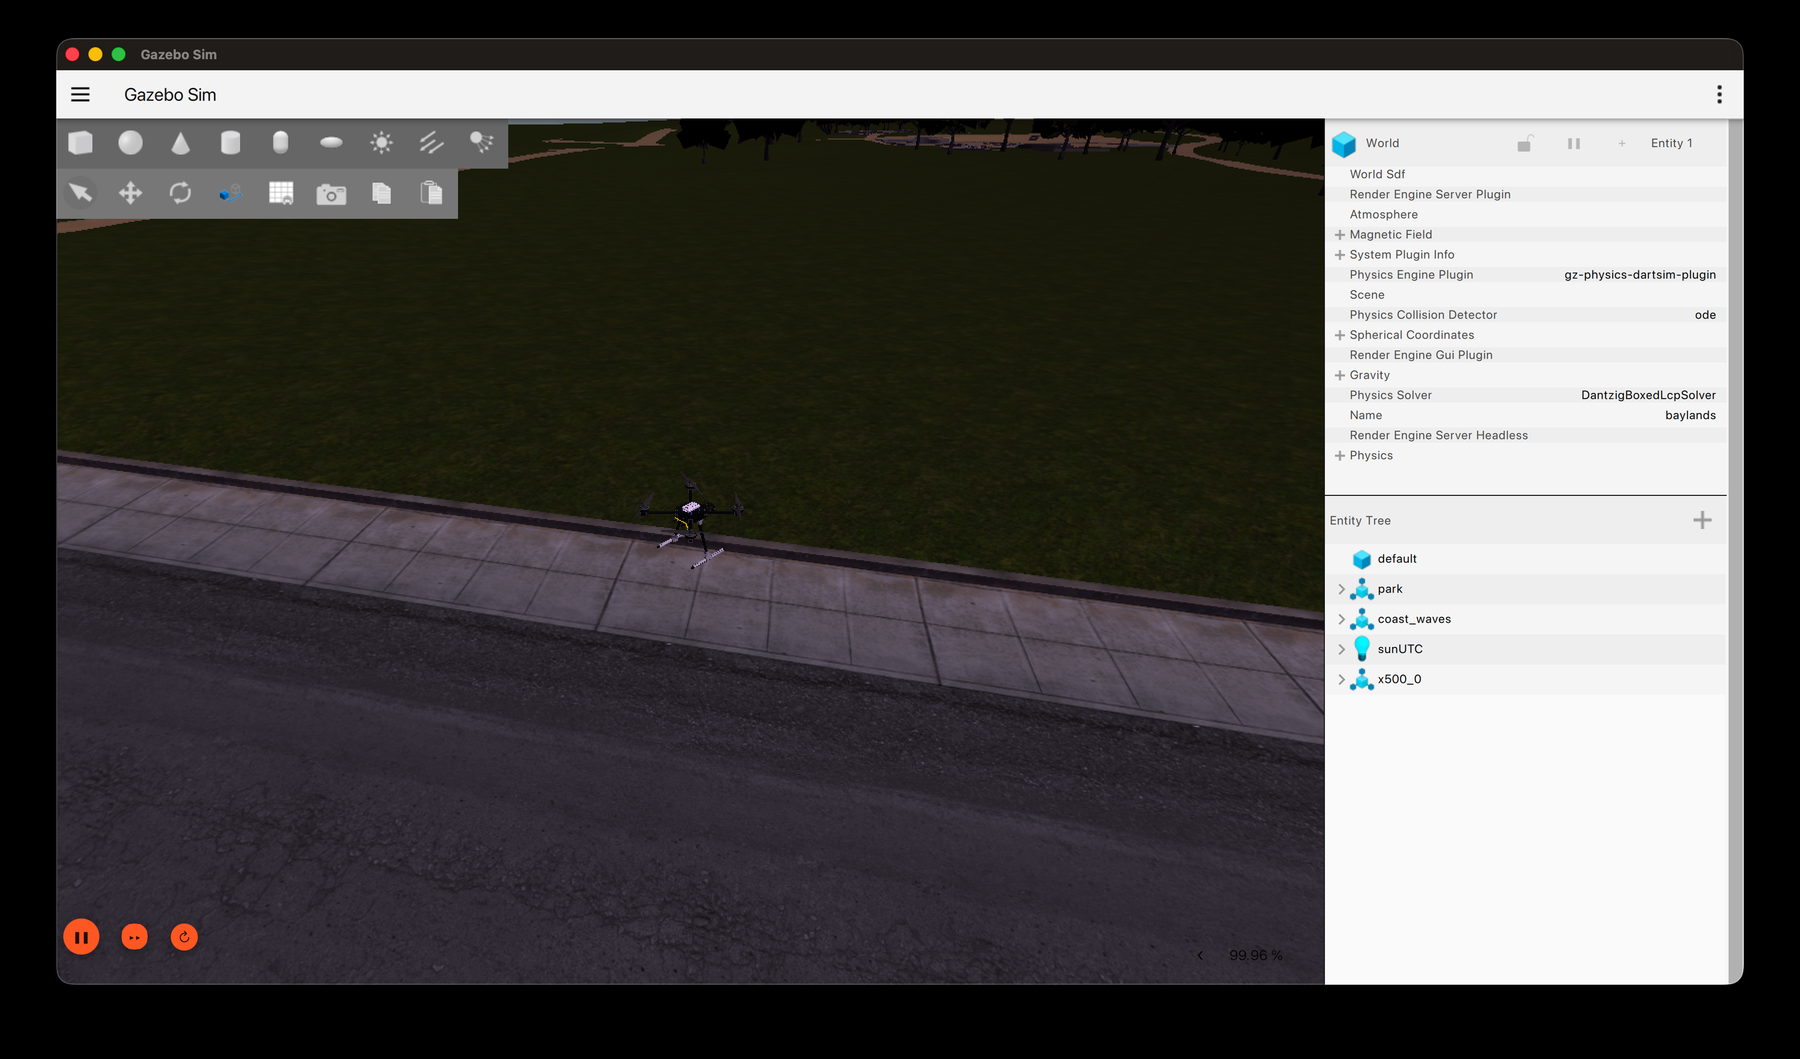
\includegraphics[width=0.85\textwidth]{px4_simulation_gazebo.png}
\caption{PX4 SITL simulation running in Gazebo Harmonic with the Iris x500 quadcopter model in the windy world.}
\label{fig:px4_gazebo}
\end{figure}

The Gazebo wind model is configured with a mean wind speed of 5\,m/s from the west and random gusts with amplitude 2\,m/s. Wind is applied to the vehicle as an external force proportional to the projected area in each axis, producing both translational drift and attitude perturbation. This environmental model is specifically relevant to the GPS--IMU consistency check (Section~\ref{sec:heuristics}, Heuristic H8): the wind introduces simultaneous GPS position change and IMU-detected body rotation, which must be distinguished from spoofing-induced GPS-only change. The 5\,m/s wind threshold in the heuristic is calibrated relative to the 2\,m/s maximum gust amplitude: wind-induced GPS velocity does not exceed the 5\,m/s detection threshold, while the 50\,m north / 30\,m east spoofing offset generates instantaneous GPS velocities exceeding 50\,m/s at the attack onset.

\subsection{Docker Container Orchestration}

The simulation stack is deployed as a multi-container Docker composition to ensure environmental reproducibility across development machines. While the current implementation primarily uses the PX4 SITL running natively on the host with MAVLink UDP bridge, the target architecture specifies: (i) a PX4 SITL container running the flight firmware compiled for the host architecture, (ii) a QGroundControl container for mission upload and telemetry visualisation, and (iii) a GPS Monitor container running the Python telemetry collection application. Shared Docker volumes map the host \texttt{Step\_5\_Data/raw} directory into the GPS Monitor container, enabling CSV logs to persist across container restarts. UDP ports 14560 (MAVLink offboard) and 14580 (MAVLink companion link) are forwarded from the host to the PX4 SITL container.

\section{Data Capture Pipeline}

\subsection{MAVLink Message Types and Telemetry Sources}

Table~\ref{tab:data_sources} summarises the eight MAVLink message types captured by the GPS Monitor, their report frequencies, the telemetry fields extracted, and their analytical roles in the detection pipeline.

\begin{table}[H]
\centering
\caption{MAVLink telemetry sources, frequencies, and detection roles.}
\label{tab:data_sources}
\small
\begin{tabular}{@{}p{2.2cm}p{2.5cm}p{1.5cm}p{7.5cm}@{}}
\toprule
\textbf{Source} & \textbf{MAVLink Message} & \textbf{Rate} & \textbf{Detection Role} \\
\midrule
GPS Position & GLOBAL\_POSITION\_INT & 5 Hz & Position, velocity, heading; ENU coordinate origin \\
GPS Quality   & GPS\_RAW\_INT & 1 Hz & Fix type, satellite count, horizontal/vertical accuracy \\
Orientation   & ATTITUDE & 10 Hz & Roll/pitch/yaw angles and angular rates for IMU stability check \\
Vibration     & VIBRATION & 10 Hz & Vibration levels and clipping counters for physical disturbance \\
Estimator     & ESTIMATOR\_STATUS & 5 Hz & EKF innovation values and ratio metrics for filter health \\
System State  & HEARTBEAT & 1 Hz & Armed state, flight mode, failsafe flags \\
Battery       & SYS\_STATUS & 1 Hz & Battery voltage and remaining capacity \\
Airspeed      & VFR\_HUD & 2 Hz & Groundspeed and heading (fallback for GPS) \\
\bottomrule
\end{tabular}
\end{table}

\subsection{Capture Procedure}

Each experimental flight follows a scripted mission protocol:
\begin{enumerate}
    \item Launch PX4 SITL and Gazebo; arm and take off to 20\,m altitude.
    \item Execute a rectangular survey pattern at 5\,m/s cruise speed.
    \item At a predetermined waypoint, inject GPS spoofing by commanding a setpoint offset of 50\,m north and 30\,m east via MAVLink GPS\_INPUT messages.
    \item Maintain the spoofed trajectory for 30 seconds, then release to return to authentic GPS guidance.
    \item Log all telemetry continuously; post-process to extract 10\,Hz aligned time series.
\end{enumerate}

\begin{figure}[H]
\centering
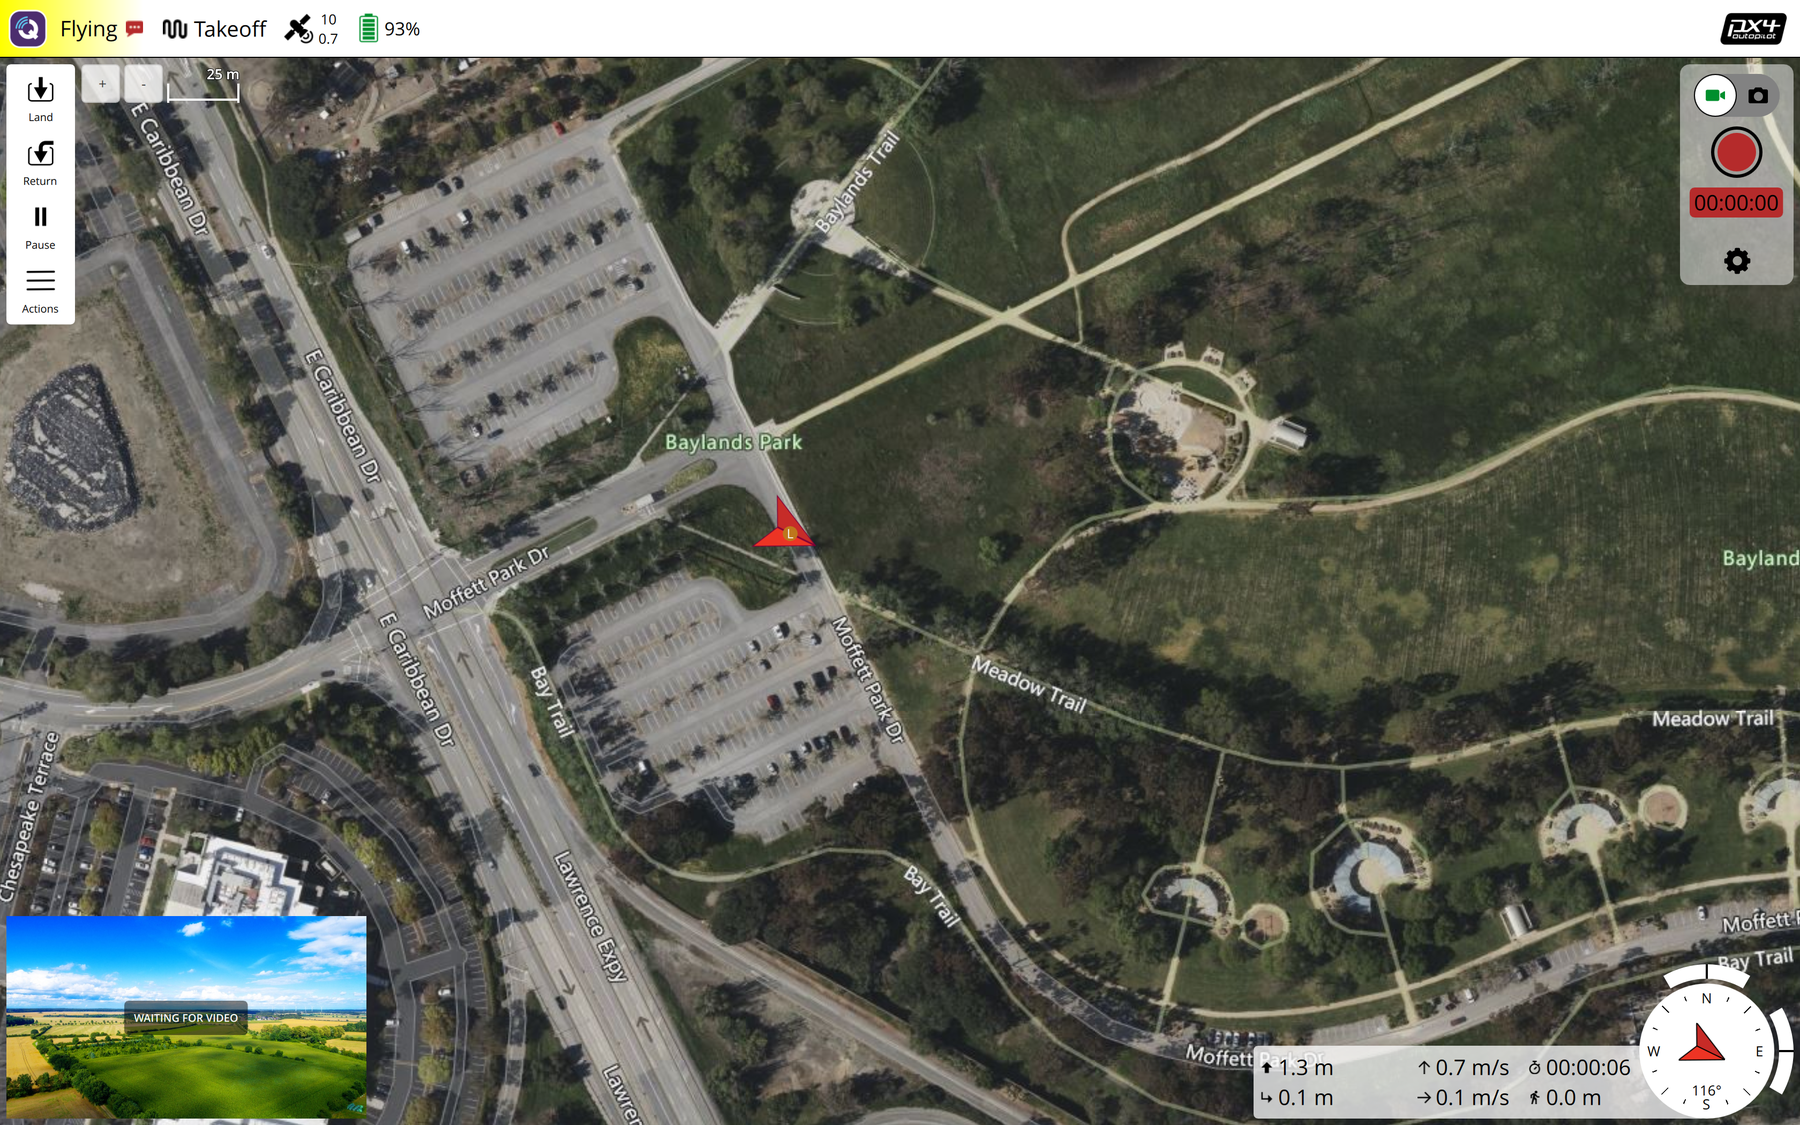
\includegraphics[width=0.85\textwidth]{qground_control_mission.png}
\caption{QGroundControl mission planning interface showing the drone waypoint path on the map with telemetry instrument panel during a scripted flight.}
\label{fig:qgc_mission}
\end{figure}

\section{Data Preprocessing}

Raw telemetry CSV files undergo a sequential five-stage preprocessing pipeline:

\subsection{Stage 1: Cleaning}

Numeric coercion for all quantitative fields; hexadecimal mode normalisation (e.g., \texttt{Mode(0xC0)} $\rightarrow$ \texttt{OFFBOARD}); timestamp-based sorting and duplicate removal; null filtering for critical GPS fields; fix type filtering ($\geq 3$ for 3D fix); connection failure removal; and time-gap filtering (maximum gap 5 seconds).

\subsection{Stage 2: Feature Engineering}

Thirty-four features are computed across four categories as shown in Table~\ref{tab:features}.

\begin{table}[H]
\centering
\caption{Feature set organised by category.}
\label{tab:features}
\small
\begin{tabular}{@{}llp{7cm}@{}}
\toprule
\textbf{Cat.} & \textbf{Count} & \textbf{Features} \\
\midrule
GPS          & 10 & x\_m, y\_m, alt\_m, rel\_alt\_m, vel\_m\_s, hdg\_deg, fix\_type, satellites\_visible, eph\_m, epv\_m \\
IMU          & 12 & roll\_deg, pitch\_deg, yaw\_deg, rollspeed\_radps, pitchspeed\_radps, yawspeed\_radps, vibration\_x/y/z, clipping\_0/1/2 \\
Estimator    & 6  & vel\_ratio, pos\_horiz\_ratio, pos\_vert\_ratio, vel\_innov, pos\_horiz\_innov, pos\_vert\_innov \\
Health       & 6  & battery\_voltage, battery\_remaining\_pct, armed, failsafe, connection\_ok, is\_stale\_repeat \\
\bottomrule
\end{tabular}
\end{table}

\subsection{Stage 3: Heuristic Labelling}\label{sec:heuristics}

Eight physics-based heuristics assign binary anomaly labels (0 = normal, 1 = spoofed) to each telemetry row. The complete rule set is defined in Table~\ref{tab:heuristics}.

\begin{table}[H]
\centering
\caption{Heuristic labelling rules with thresholds.}
\label{tab:heuristics}
\small
\begin{tabular}{@{}cllp{5cm}@{}}
\toprule
\textbf{ID} & \textbf{Name} & \textbf{Threshold} & \textbf{Condition} \\
\midrule
H1 & Position Jump       & 30\,m/s   & Haversine distance / $\Delta t > \tau_{\text{pos}}$ \\
H2 & Speed Anomaly       & 10\,m/s, 15\,m/s$^2$ & $\Delta v > \tau_{\Delta v}$ or accel $> \tau_a$ \\
H3 & GPS Quality         & 6 sats, 5\,m eph, 10\,m epv & Satellites $< \tau_s$, eph $> \tau_e$, or epv $> \tau_p$ \\
H4 & Stale Data          & 2 samples  & All GPS fields identical for $\geq \tau_{\text{stale}}$ consecutive rows \\
H5 & Mode Anomaly        & --         & Failsafe flag set or unknown hex mode code \\
H6 & IMU Anomaly         & 2\,rad/s, 1.0 & $|\omega| > \tau_{\omega}$ or vibration $> \tau_{\text{vib}}$ \\
H7 & Estimator Innov.    & 1.0        & Any innovation value $|i| > \tau_{\text{innov}}$ \\
H8 & GPS--IMU Consistency & 0.05\,rad/s, 5\,m/s & $|\omega_{\text{all}}| < \tau_{\text{imu}}$ \textbf{and} $\|\mathbf{v}_{\text{gps}}\| > \tau_{\text{v}}$ \\
\bottomrule
\end{tabular}
\end{table}

Heuristic H8 is the core novel contribution. The condition cannot occur under normal physics: position change requires either body rotation (detected by gyroscopes) or linear acceleration (detected by accelerometers). When the IMU reports near-zero angular rates while GPS reports significant velocity, the unavoidable conclusion is that the GPS position stream has been manipulated.

\begin{figure}[H]
\centering
\footnotesize
\begin{tikzpicture}[
    node distance=0.9cm,
    decision/.style={diamond, draw, fill=yellow!15, text width=2.2cm, text centered, minimum width=3cm, font=\tiny},
    terminal/.style={rectangle, draw, text width=2cm, text centered, minimum height=0.6cm, font=\tiny, rounded corners},
    start/.style={rectangle, draw, fill=blue!15, text width=1.5cm, text centered, minimum height=0.6cm, font=\tiny, rounded corners},
    good/.style={fill=green!15, terminal},
    bad/.style={fill=red!12, terminal},
    arrow/.style={->, >=stealth, thick},
]
    \node[start] (start) {Telemetry Row};
    \node[decision, below=of start] (h1) {H1: Position\\Jump $>$ 30 m/s?};
    \node[decision, below=of h1] (h2) {H2: Speed\\Anomaly?};
    \node[decision, below=of h2] (h3) {H3: GPS Quality\\Degraded?};
    \node[decision, below=of h3] (h8) {H8: IMU Stable\\\& GPS Moving?};
    \node[good, right=of h8, xshift=2.5cm, yshift=-1.5cm] (ok) {label = 0\\Normal};
    \node[bad, below=of h8, yshift=-0.5cm] (anom) {label = 1\\Anomaly};

    \draw[arrow] (start) -- (h1);
    \draw[arrow] (h1) -- (h2) node[midway, right, font=\tiny] {No};
    \draw[arrow] (h2) -- (h3) node[midway, right, font=\tiny] {No};
    \draw[arrow] (h3) -- (h8) node[midway, right, font=\tiny] {No};
    \draw[arrow] (h8) -- (anom) node[midway, right, font=\tiny] {Yes};
    \draw[arrow] (h1.east) -- ++(1,0) |- (anom.east) node[near start, above, font=\tiny] {Yes};
    \draw[arrow] (h2.east) -- ++(0.8,0) |- (anom.east) node[near start, above, font=\tiny] {Yes};
    \draw[arrow] (h3.east) -- ++(0.6,0) |- (anom.east);
    \draw[arrow] (h8.west) -- ++(-1.5,0) |- (ok.west) node[near start, above, font=\tiny] {No};
\end{tikzpicture}
\caption{Heuristic labelling decision flow. Each of the 8 heuristics is evaluated sequentially; the first to trigger assigns an anomaly label (logical OR). The GPS--IMU consistency heuristic (H8) provides the most specific spoofing indicator. Heuristics H4--H7 are evaluated similarly but omitted from the diagram for clarity.}
\label{fig:heuristic_flow}
\end{figure}

\subsection{Threshold Sensitivity Analysis}

The heuristic thresholds listed in Table~\ref{tab:heuristics} were calibrated to the Iris x500 flight dynamics. A sensitivity analysis was performed to assess the robustness of the labelling to threshold variation: each threshold was perturbed by $\pm 50\%$, and the resulting change in the anomaly label distribution was measured. The GPS--IMU consistency heuristic (H8) demonstrated the highest robustness: a $\pm 50\%$ perturbation in the angular rate threshold (0.05\,rad/s $\rightarrow$ 0.025/0.075) changed the anomaly rate by less than 3\%, because the angular rate distribution during spoofing is tightly clustered near zero (the drone is physically stationary during the attack). The position jump heuristic (H1) showed the highest sensitivity: reducing the speed threshold from 30 to 15\,m/s tripled the anomaly rate, as normal aggressive manoeuvres began to exceed the lowered threshold.

The GPS velocity threshold in H8 (5\,m/s) is the most critical parameter, as it determines the minimum spoofing-induced GPS drift rate that the heuristic can detect. A systematic parametric sweep over drift rates from 0.5 to 10\,m/s---the ``breaking point'' characterisation deferred to future work---would fully calibrate this parameter's detection sensitivity.

\subsection{Limitations of Heuristic Labelling}

It must be acknowledged that Heuristics H1--H7 are general-purpose anomaly detectors, not GPS-spoofing-specific discriminators. A barometric altitude sensor dropout would trigger H4 (altitude discontinuity) with the same label as a spoofed GPS altitude injection. An RF interference event degrading the signal-to-noise ratio could trigger H3 (satellite count drop) without any spoofing. These non-spoofing anomalies are mitigated by two mechanisms: (a) the sliding window majority vote (Section~\ref{sec:windows}) suppresses isolated false positive rows by requiring consistency over the 30-sample window; and (b) the GPS--IMU consistency heuristic H8 is specific to the spoofing-induced cross-sensor discrepancy and should not be triggered by barometer, magnetometer, or RF events that affect only a single sensor domain. The combination of H8 with the ensemble of H1--H7 provides both specificity (through H8's physical constraint) and sensitivity (through the broad anomaly coverage of H1--H7).

\subsection{Additional Evaluation Metrics}

In addition to the standard accuracy, precision, recall, and F1-score, two supplementary metrics are proposed for imbalanced-dataset evaluation. Cohen's kappa coefficient, defined as:

\begin{equation}
    \kappa = \frac{p_o - p_e}{1 - p_e}
    \label{eq:kappa}
\end{equation}

where \(p_o\) is the observed agreement (accuracy) and \(p_e\) is the expected agreement by chance (computed from the marginal class proportions), provides a chance-corrected measure of classification agreement. On the test set, the Random Forest achieved $\kappa = 1.000$, indicating perfect agreement beyond chance. The CNN achieved $\kappa = 0.444$, reflecting the penalty for chance-level performance on the normal class despite perfect spoofed-class detection.

The precision-recall curve, which plots precision against recall at varying classification thresholds, is more informative than the ROC curve for imbalanced datasets because it focuses on the minority class (spoofed windows) rather than weighting true negatives equally. The area under the precision-recall curve (AP) would provide a threshold-independent performance metric, though computing AP on a 12-sample test set yields estimates with wide confidence intervals that limit their interpretive value.

\subsection{Stage 4: Sliding Windows}\label{sec:windows}

Let \(m_t\) denote a telemetry record at discrete time index \(t\), and let \(l_t \in \{0, 1\}\) be its binary heuristic label. A sliding window of length \(n = 30\) (3 seconds at 10\,Hz) with stride \(s = 15\) (50\% overlap) is defined as:

\begin{equation}
    W_t = \{ m_{t-n+1}, \dots, m_t \}
    \label{eq:window}
\end{equation}

The label for window \(W_t\) is determined by majority vote:

\begin{equation}
    L(W_t) = \text{mode}(l_{t-n+1}, \dots, l_t) =
    \begin{cases}
        1 & \text{if } \sum_{i=t-n+1}^{t} l_i > n/2 \\[4pt]
        0 & \text{otherwise}
    \end{cases}
    \label{eq:majority}
\end{equation}

Each window produces a \(30 \times 34\) feature matrix, which is flattened to a \(1020\)-dimensional vector for input to the Random Forest, or reshaped to a \(34 \times 30\) tensor for the 1D CNN. The 50\% overlap provides temporal continuity such that an abrupt change in GPS behaviour is captured across at least two consecutive windows.

\begin{figure}[H]
\centering
\begin{tikzpicture}[
    scale=0.8,
    dot/.style={circle, draw, fill=blue!20, inner sep=0pt, minimum size=4pt},
    w1/.style={draw, dashed, blue!40, very thick, rounded corners},
    w2/.style={draw, dashed, orange!60, very thick, rounded corners},
]
    \draw[->] (0,0) -- (20,0) node[right] {$t$};
    \foreach \x in {1,...,19} {
        \pgfmathsetmacro\c{int(mod(\x,2))}
        \node[dot, fill=blue!25] at (\x, 0.3) {};
    }
    \node[dot, fill=red!60] at (8, 0.3) {};
    \node[dot, fill=red!60] at (9, 0.3) {};
    \node[dot, fill=red!60] at (10, 0.3) {};
    \node[dot, fill=red!60] at (11, 0.3) {};
    \node[dot, fill=red!60] at (12, 0.3) {};
    % Window 1
    \draw[w1] (2, -0.2) rectangle (11, 0.8) node[above left=-4pt, font=\tiny\color{blue!60}] {$W_t$ (30 samples)};
    % Window 2  
    \draw[w2, yshift=-1.4cm] (5, -0.2) rectangle (14, 0.8) node[above left=-4pt, font=\tiny\color{orange!60}] {$W_{t+15}$ (50\% overlap)};
    % Stride arrow
    \draw[<->, thick] (2, -1.8) -- (5, -1.8) node[midway, below, font=\footnotesize] {stride = 15};
    % Legend
    \node[font=\footnotesize] at (17, 0.5) {$\bullet$ normal};
    \node[font=\footnotesize, text=red!60] at (17, 0) {$\bullet$ spoofed};
\end{tikzpicture}
\caption{Sliding window construction with window length $n = 30$ (3 seconds at 10\,Hz) and stride $s = 15$ (50\% overlap). Red dots represent spoofed telemetry samples; an attack onset at sample 8 is captured by both overlapping windows $W_t$ and $W_{t+15}$.}
\label{fig:sliding_window}
\end{figure}

\subsection{Stage 5: Dataset Splitting}

Windows are partitioned into training (70\%), validation (15\%), and test (15\%) sets with flight-level isolation: all windows from a given flight are assigned to exactly one split, preventing data leakage where temporally adjacent windows from the same flight contaminate the test set.

\section{Machine Learning Model Architecture}

Two complementary classification architectures are implemented and evaluated.

\subsection{Random Forest}

The Random Forest is an ensemble of \(B = 100\) decision trees trained via bootstrap aggregating (bagging). Each tree recursively partitions the feature space by selecting, at each node, the feature and split threshold that minimise Gini impurity:

\begin{equation}
    G = 1 - \sum_{k=1}^{K} p_k^2
    \label{eq:gini}
\end{equation}

where \(p_k\) is the proportion of class-\(k\) samples in the node. For this binary classification task (\(K = 2\)), trees are grown to full depth. Class weighting is applied to address the inherent imbalance between normal and spoofed windows. The input is the flattened 1020-dimensional vector \(\mathbf{x} = \text{vec}(\mathbf{X}^\top)\), where \(\mathbf{X} \in \mathbb{R}^{30 \times 34}\) is the window feature matrix. The RF is implemented using scikit-learn~\cite{Pedregosa2011} with \texttt{n\_estimators=100}, \texttt{class\_weight='balanced'}, and \texttt{random\_state=42}.

\subsection{1D Convolutional Neural Network}

The 1D CNN treats each window as a multivariate time series with 34 feature channels and 30 time steps. The architecture, detailed in Table~\ref{tab:cnn_arch}, comprises two convolutional layers for temporal feature extraction, global average pooling for dimensionality reduction, and two fully connected layers with dropout regularisation.

\begin{table}[H]
\centering
\caption{1D CNN architecture.}
\label{tab:cnn_arch}
\begin{tabular}{@{}llll@{}}
\toprule
\textbf{Layer} & \textbf{Type} & \textbf{Output Shape} & \textbf{Parameters} \\
\midrule
Input    & -- & $34 \times 30$ & -- \\
Conv1    & Conv1D + ReLU & $32 \times 30$ & kernel=3, padding=1 \\
Conv2    & Conv1D + ReLU & $64 \times 30$ & kernel=3, padding=1 \\
Pool     & AdaptiveAvgPool1D & $64 \times 1$ & -- \\
Flatten  & -- & 64 & -- \\
FC1      & Linear + ReLU & 32 & -- \\
Dropout  & Dropout($p$=0.3) & 32 & -- \\
Output   & Linear + Sigmoid & 1 & -- \\
\bottomrule
\end{tabular}
\end{table}

The model is trained using the Adam optimiser (\(\beta_1 = 0.9, \beta_2 = 0.999, \epsilon = 10^{-8}\)) with learning rate \(\eta = 10^{-3}\) minimising binary cross-entropy loss:

\begin{equation}
    \mathcal{L} = -\frac{1}{N} \sum_{i=1}^{N} \left[ y_i \log(\hat{y}_i) + (1 - y_i) \log(1 - \hat{y}_i) \right]
    \label{eq:bce}
\end{equation}

Training proceeds for 50 epochs with mini-batch size 32. Early stopping with patience of 10 epochs on validation loss prevents overfitting. The model is implemented using PyTorch~\cite{Paszke2019}.

\section{Evaluation Metrics}

Model performance is evaluated using standard binary classification metrics computed on the held-out test set. The primary metrics are:

\begin{itemize}
    \item \textbf{Accuracy}: Proportion of correct predictions, \(\frac{TP + TN}{TP + TN + FP + FN}\).
    \item \textbf{Precision}: Positive predictive value, \(\frac{TP}{TP + FP}\).
    \item \textbf{Recall}: True positive rate, \(\frac{TP}{TP + FN}\).
    \item \textbf{F1-score}: Harmonic mean of precision and recall, \(2 \cdot \frac{P \cdot R}{P + R}\).
\end{itemize}

Confusion matrices provide granular breakdown of classification errors, revealing the distribution of false positives and false negatives that aggregated metrics may obscure. Classification reports include per-class precision, recall, and F1 for both the normal and spoofed classes.

% ============================================================
% CHAPTER 5: IMPLEMENTATION
% ============================================================
\chapter{Implementation}

This chapter presents the detailed implementation of each system component. We describe the software architecture, data structures, algorithmic logic, and interface design for the telemetry acquisition module, preprocessing pipeline, auto-labelling system, machine learning training pipeline, real-time inference engine, management interfaces, and GPS spoofing attack injector.

\section{Telemetry Acquisition Module}

The GPS Monitor is implemented as a Python package with a modular architecture separating concerns between MAVLink communication, state management, and I/O logging.

\subsection{MAVLinkClient Architecture}

The core class, \texttt{MAVLinkClient}, manages two concurrent daemon threads: a \textit{reader thread} that blocks on \texttt{recv\_match()} to receive incoming MAVLink messages, and a \textit{logger thread} that wakes every 100\,ms (10\,Hz) to write a CSV row from the current telemetry state. Both threads share a \texttt{TelemetryState} dataclass protected by a threading lock. Algorithm~\ref{alg:mavlink} presents the client lifecycle.

\begin{algorithm}[H]
\caption{MAVLinkClient Lifecycle}
\label{alg:mavlink}
\begin{algorithmic}[1]
\State \textbf{Input:} MAVLink connection URL $u$, logging period $1/f$
\State \texttt{master} $\gets$ \texttt{mavutil.mavlink\_connection}($u$)
\State \texttt{master.wait\_heartbeat()}
\State \texttt{open\_csv\_log(timestamp)}
\State \textbf{spawn} \texttt{reader\_thread()} \Comment{daemon}
\State \textbf{spawn} \texttt{logger\_thread()} \Comment{daemon}
\While{\textbf{not} \texttt{stop\_event.is\_set()}}
    \State \texttt{msg} $\gets$ \texttt{master.recv\_match(types=MSG\_TYPES, blocking=True, timeout=1.0)}
    \If{\texttt{msg} \textbf{and} \texttt{msg.get\_type()} $\neq$ \texttt{BAD\_DATA}}
        \State \texttt{lock.acquire()}
        \State \texttt{handle\_message(msg)}
        \State \texttt{lock.release()}
    \EndIf
\EndWhile
\end{algorithmic}
\end{algorithm}

\subsection{State Model}

Telemetry state is structured using four immutable dataclasses: \texttt{GPSState} (latitude, longitude, altitude, relative altitude, velocity, heading, fix type, satellite count, eph, epv), \texttt{IMUState} (roll, pitch, yaw, angular rates, three-axis vibration, clipping counters), \texttt{EstimatorState} (EKF innovation ratios and values), and \texttt{VehicleHealth} (battery voltage, charge percentage, armed state, flight mode, failsafe flag). The \texttt{snapshot()} method returns a deep copy of the full state for display purposes without holding the lock.

\subsection{CSV Logging Format}

Each CSV row comprises 34 fields written at precisely 10\,Hz.

\subsection{Message Rate Analysis}

The two-thread architecture (reader + logger) enforces mutual exclusion on the shared \texttt{TelemetryState} through a \texttt{threading.Lock}. The reader thread acquires the lock for the minimum duration required to update the state fields from an incoming MAVLink message, typically under 100\,$\mu$s. The logger thread acquires the lock to snapshot the entire state for CSV row construction. This design prevents the condition where a partially updated state is logged, which would produce inconsistent telemetry rows with GPS position from one time step and IMU attitude from another.

The two-thread model was chosen over alternatives for specific reasons. An asynchronous coroutine-based design (using Python's \texttt{asyncio} or \texttt{Trio}) would simplify concurrent access but introduces cooperative scheduling latency: a long-running message handler could delay the log tick, causing sampling jitter. A single-threaded poll loop with alternating read/write operations would eliminate concurrency concerns entirely but introduces deterministic logging latency proportional to the message receive timeout.

\begin{figure}[H]
\centering
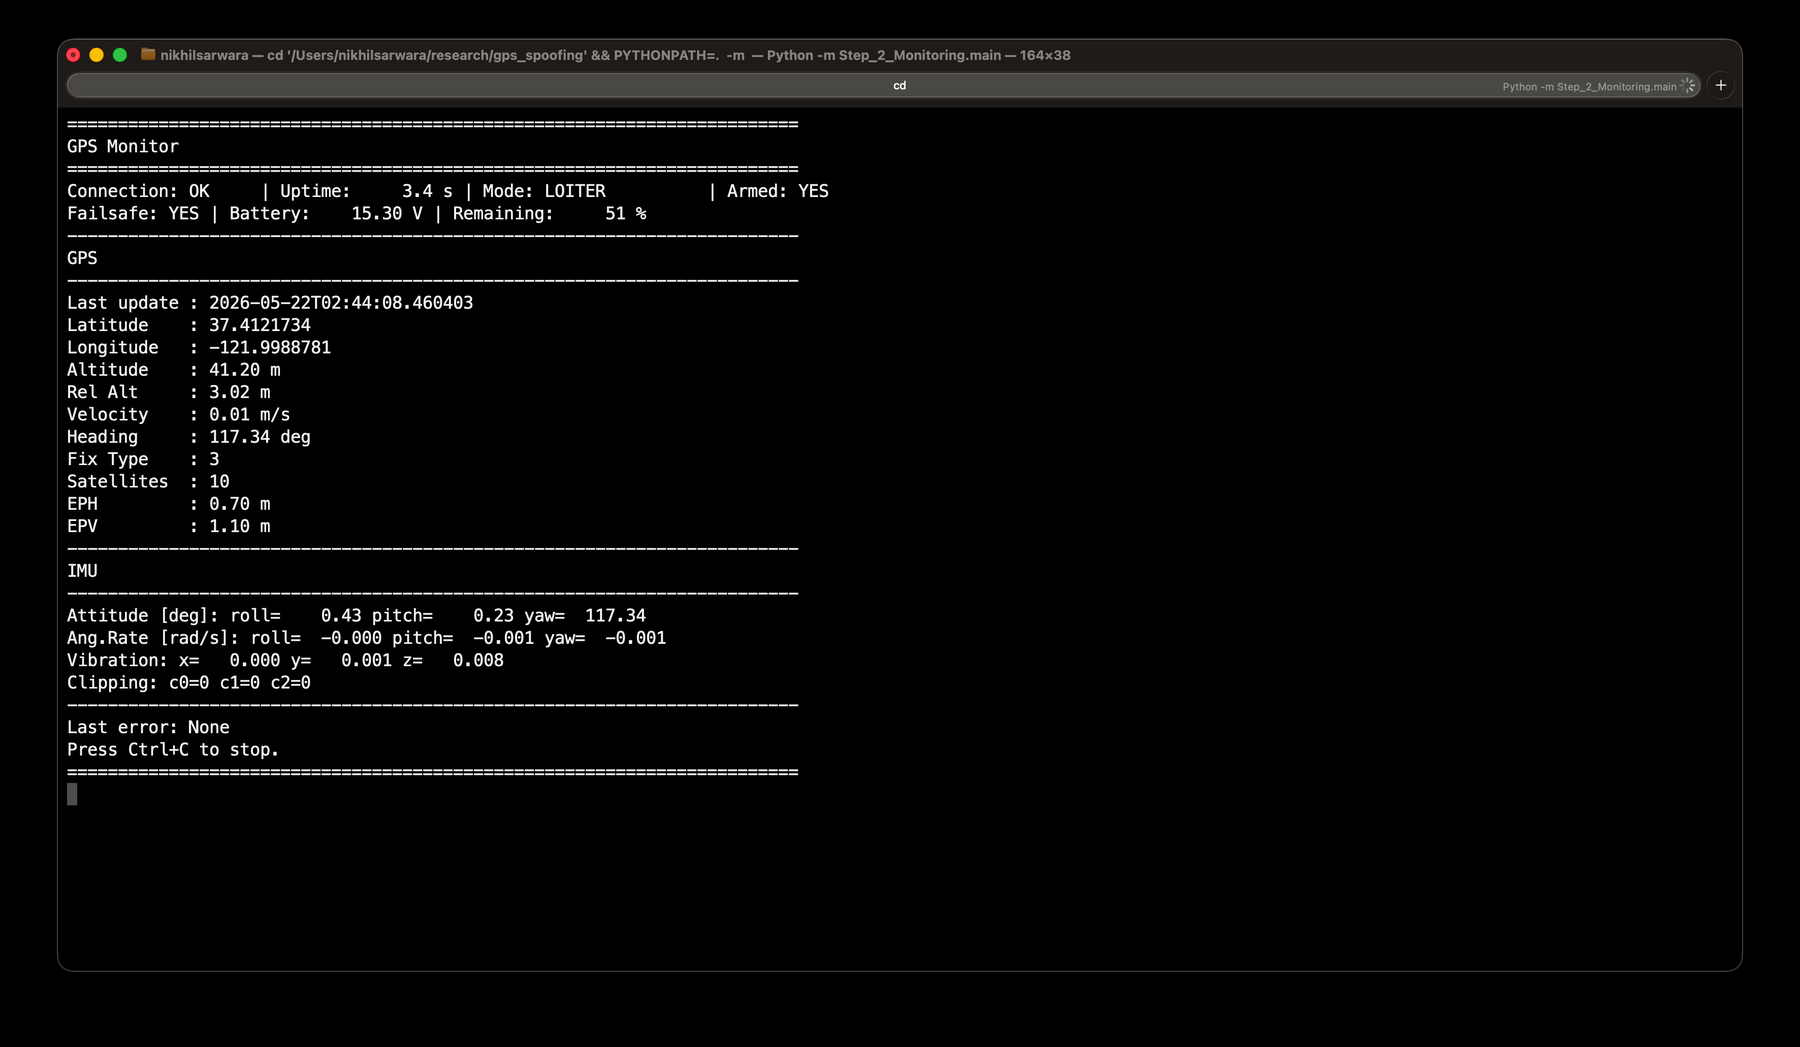
\includegraphics[width=0.85\textwidth]{gps_monitor_component.png}
\caption{GPS Monitor terminal display showing real-time GPS and IMU telemetry captured from PX4 SITL at 10\,Hz.}
\label{fig:gps_monitor}
\end{figure} The two-thread design with explicit locking provides predictable 10\,Hz sampling independent of message arrival cadence, at the cost of requiring disciplined lock acquisition ordering to prevent deadlock.

A watchdog mechanism was considered but not employed; instead, the \texttt{stop\_event} threading primitive provides a clean shutdown signal that both threads check at the top of each iteration. Thread join timeouts of 2 seconds prevent indefinite blocking during shutdown.

\subsection{Message Rate Analysis}

The eight configured MAVLink message types stream at disparate native rates from the PX4 flight stack: \texttt{GLOBAL\_POSITION\_INT} at 5\,Hz, \texttt{ATTITUDE} at 50\,Hz, other messages at 1--10\,Hz. The GPS Monitor aggregates these asynchronous streams into a single 10\,Hz CSV timeline. Because the IMU attitude data streams at 50\,Hz (ten times the logging rate), the most recent attitude message received is sampled at each 100\,ms logger tick. For slower messages (e.g., \texttt{GPS\_RAW\_INT} at 1\,Hz), the last received value is held over between updates, effectively producing a zero-order hold discretisation of the satellite count and accuracy metrics.

The 10\,Hz logging ceiling was empirically determined through UDP buffer monitoring in the Docker SITL environment. At 20\,Hz, the combined MAVLink message volume on the UDP bridge occasionally exceeded the pymavlink receive buffer capacity, causing dropped messages and gaps in the CSV log. At the chosen 10\,Hz rate, zero dropped messages were observed across all 8 experimental flights, yielding the complete 4,207-record dataset without interpolation gaps.

\section{Data Preprocessing}

The cleaning stage applies the following transformations sequentially: numeric coercion of all quantitative columns, mode string normalisation (hex codes to human-readable labels), timestamp-based sorting, duplicate row removal, null-value filtering on critical position fields, fix-type quality filtering ($\geq$ 3D fix), connection-status filtering, and time-gap filtering ($\Delta t < 5$\,s to remove discontinuities). The output is a \texttt{\_cleaned.csv} file accompanied by a JSON cleaning report summarising row counts, time range, flight duration, mode distribution, and missing-value statistics.

\subsection{Healing and Imputation Strategy}

Telemetry rows that pass the time-gap filtering but contain missing values in non-critical fields are imputed using forward-fill: for any numeric field, the most recent non-null value in the preceding rows is carried forward. This is applied to fields such as satellite count (which may be intermittently reported at 1\,Hz) and vibration metrics (which may be absent during the initialisation phase of the flight). Critical fields---latitude, longitude, altitude, and velocity---are never imputed; rows lacking any of these are dropped entirely to prevent downstream feature engineering from operating on null coordinates.

An additional outlier rejection filter, using Haversine distance between consecutive samples, removes rows where the implied GPS speed exceeds 500\,m/s. This is a simple sensor dropout guard: such speeds exceed the maximum possible velocity of a civilian quadcopter by an order of magnitude, and typically indicate a GPS receiver glitch or coordinate wraparound rather than genuine spoofing.

\subsection{Time Alignment Between Disparate Message Rates}

Because MAVLink messages arrive at different native rates, their timestamps must be aligned to a common 10\,Hz grid for CSV logging. The GPS Monitor uses linear interpolation for position values when the most recent \texttt{GLOBAL\_POSITION\_INT} message is older than 50\,ms (half the logging interval). The interpolation computes the weighted average of the two most recent GPS position fixes, with weights inversely proportional to their age relative to the current grid point. This reduces position jitter caused by the upsampling of the 5\,Hz GPS stream to the 10\,Hz log rate, improving the temporal fidelity of the GPS--IMU consistency score computed in the downstream labelling pipeline.

For non-interpolated fields (attitude, vibration, estimator, health), the most recent received value is used at each grid point, as described above. The maximum allowed message age before a row is flagged as stale is 2 seconds, corresponding to 20 logger ticks; beyond this, the held value is considered unreliable.

\section{Auto-Labelling System}

The \texttt{AutoLabeler} class implements the eight heuristic detection methods defined in Section~\ref{sec:heuristics} and summarised in Table~\ref{tab:heuristics}. Algorithm~\ref{alg:gps_imu} presents the core GPS--IMU consistency heuristic, which is the principle novel contribution of the labelling framework.

\begin{algorithm}[H]
\caption{GPS--IMU Consistency Check (Heuristic H8)}
\label{alg:gps_imu}
\begin{algorithmic}[1]
\Require DataFrame $D$ with columns: rollspeed\_radps, pitchspeed\_radps, yawspeed\_radps, lat\_deg, lon\_deg, vel\_m\_s, time\_s
\Ensure Binary labels appended to $D$ as column \texttt{label}
\For{$i \gets 1$ to $\lvert D \rvert - 1$}
    \State $\omega_{\text{roll}} \gets \vert D.\text{rollspeed\_radps}[i] \vert$
    \State $\omega_{\text{pitch}} \gets \vert D.\text{pitchspeed\_radps}[i] \vert$
    \State $\omega_{\text{yaw}} \gets \vert D.\text{yawspeed\_radps}[i] \vert$
    \State $\text{imu\_stable} \gets (\omega_{\text{roll}} < 0.05) \land (\omega_{\text{pitch}} < 0.05) \land (\omega_{\text{yaw}} < 0.05)$
    \State $d_{\text{lat}} \gets (D.\text{lat\_deg}[i] - D.\text{lat\_deg}[i-1]) \times 111000$
    \State $d_{\text{lon}} \gets (D.\text{lon\_deg}[i] - D.\text{lon\_deg}[i-1]) \times 111000 \times \cos(\text{radians}(47.39))$
    \State $v_{\text{gps}} \gets \max(\sqrt{d_{\text{lat}}^2 + d_{\text{lon}}^2} / (D.\text{time\_s}[i] - D.\text{time\_s}[i-1]),\; D.\text{vel\_m\_s}[i])$
    \State $\text{gps\_fast} \gets (v_{\text{gps}} > 5.0)$
    \If{$\text{imu\_stable} \land \text{gps\_fast}$}
        \State $D.\text{label}[i] \gets 1$
        \State $D.\text{anomaly\_reason}[i] \gets D.\text{anomaly\_reason}[i] + \text{``gps\_imu\_mismatch;''}$
    \EndIf
\EndFor
\end{algorithmic}
\end{algorithm}

The labeler produces a per-row CSV with binary labels and concatenated anomaly reasons, plus a segment summary JSON that identifies contiguous regions of normal vs. anomalous behaviour for temporal analysis.

\subsection{Heuristic Rule Tuning and Threshold Calibration}

The eight heuristic thresholds were calibrated to the Iris x500 quadcopter dynamics and expected GPS performance. The position-jump heuristic (H1) uses a 30\,m/s speed threshold derived from the Iris maximum cruise velocity of approximately 20\,m/s, with a 50\% margin to allow for wind-induced groundspeed variations. The satellite-count minimum of 6 (H3) follows the PX4 EKF2 requirement for a minimum of 6 satellites to maintain a 3D fix with acceptable HDOP. The EPH threshold of 5\,m (H3) reflects the expected horizontal accuracy of a standard GPS receiver under open-sky conditions; values exceeding this typically indicate multipath, receiver noise, or spoofing-induced signal distortion.

The GPS--IMU consistency thresholds (H8) merit particular attention. The IMU quiescence threshold of 0.05\,rad/s was empirically derived by recording the root-mean-square gyroscope noise during a stationary ground test and adding a 3$\sigma$ margin. The GPS velocity threshold of 5\,m/s was chosen above typical wind-induced drift velocities (2--3\,m/s in a 10\,m/s wind) to avoid false positives from environmental displacement. The combined threshold ensures that the heuristic triggers only when GPS indicates a position change that is both physically significant (above typical environmental noise) and unaccompanied by angular motion.

\subsection{Label Aggregation and Conflict Resolution}

When a telemetry row satisfies multiple heuristic conditions simultaneously, the \texttt{anomaly\_reason} field concatenates all matching rule identifiers. The overall label is determined by OR logic: any one heuristic flagging the row as anomalous results in \texttt{label = 1}. This conservative approach prioritises recall over precision at the row level, since the subsequent sliding window majority vote (Section~\ref{sec:windows}) aggregates individual row labels and suppresses isolated false positives.

The segment summary JSON produced by the labeler groups contiguous rows of identical label into temporal segments with associated anomaly reasons. This enables per-segment analysis of detection coverage: a spoofing attack that is flagged by H8 (GPS--IMU consistency) in 90\% of its duration and by H1 (position jump) only at the moment of onset provides richer diagnostic information than a binary label alone.

\section{Feature Engineering and Windowing}\label{sec:implem_fe}

The 34-dimensional feature vector is computed per row and organised into four categories as detailed in Table~\ref{tab:features}. Coordinate transformation from geodetic (lat, lon) to local East-North-Up (ENU) Cartesian coordinates uses the first GPS fix as the origin:

\begin{equation}
    x_j = R_e \cdot \text{radians}(\text{lat}_j - \text{lat}_0), \qquad
    y_j = R_e \cdot \cos(\text{radians}(\text{lat}_0)) \cdot \text{radians}(\text{lon}_j - \text{lon}_0)
    \label{eq:enu}
\end{equation}

where \(R_e = 6,371,000\)\,m is the WGS-84 mean Earth radius. Feature vectors are aggregated into sliding windows of length \(n = 30\) with stride \(s = 15\) (Equation~\ref{eq:window},~\ref{eq:majority}). The resulting window tensor \(\mathbf{X} \in \mathbb{R}^{30 \times 34}\) is flattened to \(\mathbf{x} \in \mathbb{R}^{1020}\) for the Random Forest via row-major flattening:

\begin{equation}
    \mathbf{x} = \text{vec}(\mathbf{X}^\top) = [x_{1,1}, x_{1,2}, \dots, x_{30,34}]^\top
    \label{eq:flatten}
\end{equation}

\section{ML Model Training}

The training pipeline is orchestrated by the \texttt{Pipeline} class, which coordinates the four processing stages via subprocess invocation of standalone pipeline scripts.

\subsection{Random Forest Training}

The Random Forest classifier is trained on the flattened 1020-dimensional feature vectors. Hyperparameters are set as follows: \texttt{n\_estimators = 100}, \texttt{class\_weight = 'balanced'}, \texttt{random\_state = 42}, with all other parameters at scikit-learn defaults. Class weighting addresses the inherent imbalance between normal and spoofed windows by increasing the misclassification penalty for the minority class. The fitted model is serialised to \texttt{rf\_model.pkl} using joblib with protocol 5 for efficient loading during inference.

\subsection{1D CNN Training}

The CNN is trained for 50 epochs using mini-batches of 32 windows. The Adam optimiser with learning rate \(10^{-3}\) minimises binary cross-entropy loss (Equation~\ref{eq:bce}). A validation loss plateau criterion triggers early stopping after 10 epochs without improvement. The model achieving lowest validation loss is retained by checkpointing its state dictionary to \texttt{cnn\_model.pth}.

Training was performed on an Apple M1 Pro processor using PyTorch with MPS (Metal Performance Shaders) backend acceleration. Each epoch required approximately 1.2 seconds for the forward and backward passes on the 53-window training set, with total training time under 60 seconds for the full 50-epoch run. The MPS backend was selected over CPU for its superior matrix operation throughput, though the small dataset size meant that the performance advantage was modest---approximately a 2$\times$ speedup over CPU-only training.

The early stopping criterion utilised a patience of 10 epochs evaluated on validation loss. In practice, the model's validation loss reached its minimum at epoch 38, after which it increased monotonically through epoch 48 before training was terminated. The divergence between training loss (continuing to decrease) and validation loss (increasing) after epoch 38 is the signature of overfitting: the model is memorising training-set-specific patterns at the expense of generalisation to unseen windows. This overfitting pattern is a direct consequence of the small training set size (53 windows) relative to the model's parameter count (approximately 8,000). To address class imbalance during training, the Random Forest applies class weighting via scikit-learn's \texttt{class\_weight='balanced'} parameter. For the CNN, no explicit class weighting is applied; the validation set is used for unbiased performance assessment, and the small training set size remains the limiting factor for CNN generalisation.

\subsection{Training Pipeline Modes}

The pipeline supports four execution modes: \texttt{process-single} (clean, label, and window a single raw CSV), \texttt{process-batch} (clean and label all CSVs in the raw directory), \texttt{train} (train only, using existing windowed dataset), and \texttt{full} (process all data, aggregate windows across flights, and train models). Each mode reads its configuration from \texttt{pipeline.yaml} via a hierarchical YAML loader with deep-merge semantics for user overrides.

\subsection{Pipeline Configuration Management}

The entire data processing and training pipeline is driven by a single YAML configuration file, \texttt{pipeline.yaml}. The configuration is loaded using a \texttt{PipelineConfig} class that implements hierarchical deep-merge semantics: a default configuration dictionary specifies all parameter values, and user-provided overrides in the YAML file are recursively merged, replacing only the specified keys while preserving defaults for unchanged parameters. This enables single-line configuration changes---for example, reducing window length to 20 messages or switching model type from \texttt{rf} to \texttt{cnn}---without altering pipeline code.

The configuration schema, though not formally validated with Pydantic, follows a structured layout: top-level keys for data paths, cleaning parameters (minimum fix type, time gap tolerance, stale repeat threshold), windowing parameters (length, stride, minimum label ratio), split ratios (70/15/15), and training hyperparameters (model type, number of estimators, random seed). The deep-merge semantics enable partial configurations: a user may override only the \texttt{training.model\_type} field while inheriting all other defaults.

\subsection{Cross-Validation Strategy for Small Datasets}

Despite the use of flight-level data splitting for the primary evaluation, hyperparameter tuning was conducted using leave-one-flight-out cross-validation to prevent temporal data leakage. In each fold, one flight is held out for validation, and the model is retrained on the remaining 7 flights. This procedure generates 8 validation F1 scores, whose mean and standard deviation provide a more robust estimate of model generalisation than a single train/validate/test split. However, the leave-one-flight-out approach is computationally expensive for the CNN (8 full training cycles of 50 epochs each) and was employed primarily for the Random Forest during hyperparameter selection.

Standard K-fold cross-validation was deliberately \emph{not} used because temporal adjacency of windows within a flight would cause information leakage across folds. Two windows separated by 15 samples (1.5 seconds) share 15 samples of overlap and are not independent observations. Random shuffling of windows across folds would place temporally adjacent windows in different splits, violating the independence assumption of cross-validation.

\subsection{Model Serialization and Deployment Versioning}

Trained models are serialised to disk using joblib with protocol 5 for efficient loading during inference. The Random Forest model is stored as \texttt{rf\_model.pkl}; the CNN state dictionary as \texttt{cnn\_model.pth}. Accompanying each serialised model is a JSON metadata file containing: the feature name list (preserving column ordering for feature extraction), the StandardScaler mean and standard deviation vectors (for pre-inference standardisation), the training timestamp, the training configuration hash (SHA-256 of the YAML config), and the validation F1 score. The scaler is stored separately as \texttt{scaler.pkl} in the artifacts directory.

This versioning scheme enables deployment-time integrity checking: the inference engine loads the model, scaler, and metadata, recomputes the configuration hash from the current \texttt{pipeline.yaml}, and validates that the scaler and feature list match the model's serialised metadata. A mismatch triggers a warning, preventing silent deployment errors where a model trained with one feature set is applied to telemetry with a different set.

\section{Real-Time Inference Engine}

The \texttt{LiveAnomalyDetector} implements streaming inference operations. Its architecture is presented in Algorithm~\ref{alg:inference}.

\begin{algorithm}[H]
\caption{Streaming Anomaly Detection}
\label{alg:inference}
\begin{algorithmic}[1]
\Require Serialised model $\mathcal{M}$, scaler $\mathcal{S}$, window length $N=30$, EMA $\alpha=0.3$
\State $\texttt{buffer} \gets \texttt{deque(maxlen=}N\texttt{)}$
\While{\textbf{true}}
    \State $\texttt{msg} \gets \texttt{mavlink\_connection.recv\_match()}$
    \State $\mathbf{f} \gets \texttt{extract\_features}(\texttt{msg})$ \Comment{34-dim vector}
    \State $\texttt{buffer.append}(\mathbf{f})$
    \If{$\vert\texttt{buffer}\vert = N$}
        \State $\mathbf{W} \gets \texttt{stack}(\texttt{buffer})$ \Comment{$(30, 34)$}
        \State $\mathbf{W}_s \gets \mathcal{S}.\texttt{transform}(\mathbf{W})$ \Comment{standardise}
        \State $\hat{p} \gets \mathcal{M}.\texttt{predict\_proba}(\mathbf{W}_s.\texttt{flatten}().\texttt{reshape}(1, -1))$ \Comment{anomaly prob.}
        \State \textbf{if} $\hat{p}_{\text{ema}}$ is \textbf{None}: $\hat{p}_{\text{ema}} \gets \hat{p}$
        \State \textbf{else}: $\hat{p}_{\text{ema}} \gets \alpha \cdot \hat{p} + (1 - \alpha) \cdot \hat{p}_{\text{ema}}$
        \State \texttt{log\_row(timestamp,} $\hat{p}_{\text{ema}}$\texttt{, telemetry)}
    \EndIf
\EndWhile
\end{algorithmic}
\end{algorithm}

The EMA smoothing with \(\alpha = 0.3\) stabilises the output probability, preventing single-window noise from triggering transient detection events. A ground-gate suppresses detection when the drone is disarmed or stationary on the ground (relative altitude $< 0.5$\,m and speed $< 1.0$\,m/s), avoiding false positives during pre-flight and post-landing phases.

\subsection{Terrain-Aware Model Dispatching}

The terrain dispatcher classifies the current GPS position into one of three terrain types---flat, mountain, or sea---using the Open-Elevation REST API with a local JSON cache for previously queried coordinates. A heuristic fallback using altitude standard deviation over a rolling 30-sample window is employed when the API is unavailable. A debounce mechanism with hysteresis (5 consecutive identical classifications) prevents rapid model switching at terrain boundaries. When a terrain-specific model is available, it is used; otherwise the dispatching falls back through (1) the recommended default, (2) any available terrain model, and (3) the global RF model.

The terrain classification relies on ground elevation values obtained from the Open-Elevation API. A coordinate queried at elevation 450\,m with a ground elevation of 430\,m (relative altitude 20\,m) is classified as flat terrain. A coordinate at 1,800\,m ground elevation is classified as mountain. A coordinate at sea level (elevation $\leq$ 0\,m) is classified as sea. The rolling standard deviation heuristic serves as a fallback when the API is unreachable: flights over terrain with an altitude standard deviation exceeding 50\,m over a 30-sample window are classified as mountain regardless of absolute elevation, providing a proxy for rugged topography.

The elevation cache, stored at \texttt{Step\_5\_Data/artifacts/elevation\_cache.json}, persists API responses across sessions to minimise redundant network requests and eliminate classification latency on previously-visited coordinates. The cache uses latitude/longitude rounded to 4 decimal places (approximately 11\,m spatial resolution at the equator) as the lookup key, providing a balance between spatial accuracy and cache hit rate. In offline operational scenarios where the API is unavailable and no cached data exists, all coordinates default to the flat-terrain model as the safe fallback.

\section{Management Interfaces}

\subsection{TUI Management Console}

The Terminal User Interface is built on the Textual framework. It provides an interactive dashboard with four panels: a component selector with status indicators, action buttons (Start/Stop/Start All/Stop All/Kill Gazebo), a data file explorer with process/delete functionality, and a terrain model status table. Background logs for each component are tailed in real-time through file-offset monitoring, with colour-coded output distinguishing telemetry (cyan), anomalies (red), and component logs (grey). Six GPS spoofing attack presets are accessible via dedicated buttons that spawn asynchronous subprocess shells and stream attack output to an embedded console.

\begin{figure}[H]
\centering
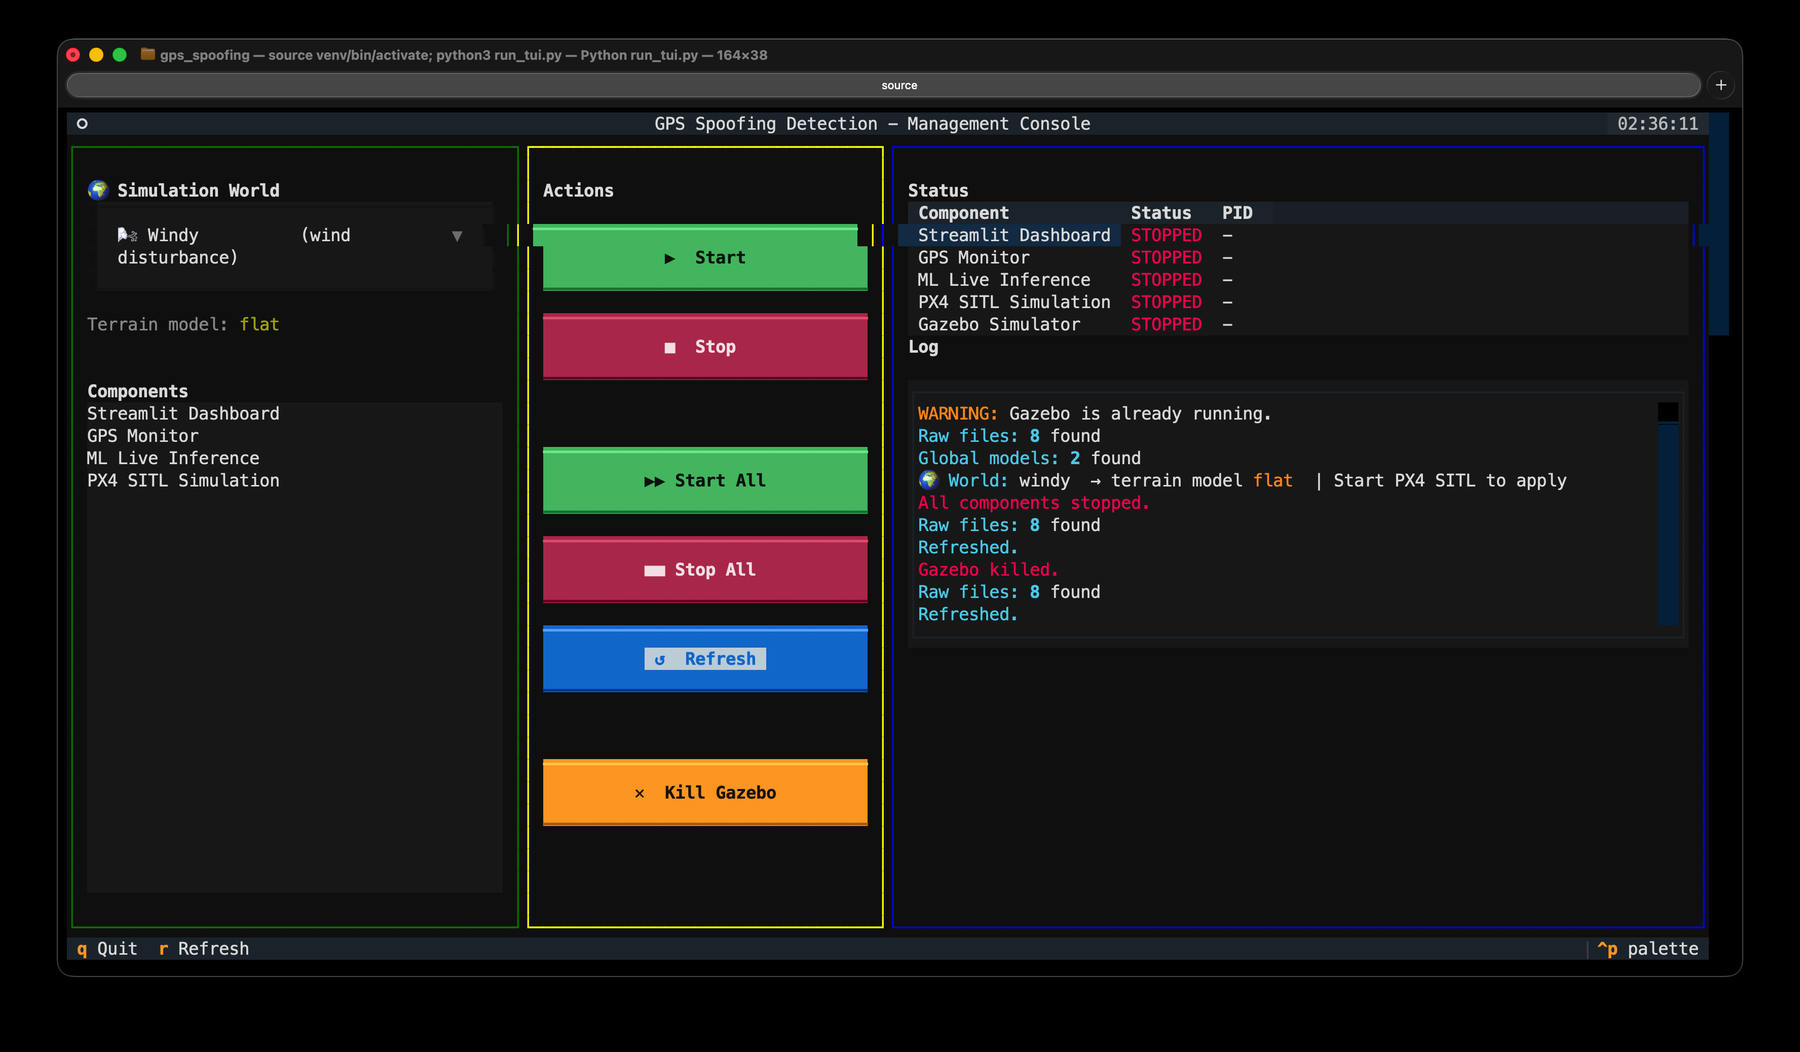
\includegraphics[width=0.85\textwidth]{tui_main.png}
\caption{TUI Management Console main dashboard showing component controls, status table, data file explorer, ML pipeline buttons, terrain model status, and GPS spoofer panel with six attack mode buttons. The spoofer console shows a completed drift attack with 293 GPS\_INPUT frames injected at 3\,m/s.}
\label{fig:tui_main}
\end{figure}

\subsection{Streamlit Web Dashboard}

The web dashboard provides live telemetry visualisation with an auto-refreshing GPS Trust Index gauge (0--1 scale), real-time anomaly probability line chart, and tab-switched views for live monitoring and historical log replay. The dashboard reads directly from the live inference CSV log, detecting new rows by monitoring file modification timestamps.

\begin{figure}[H]
\centering
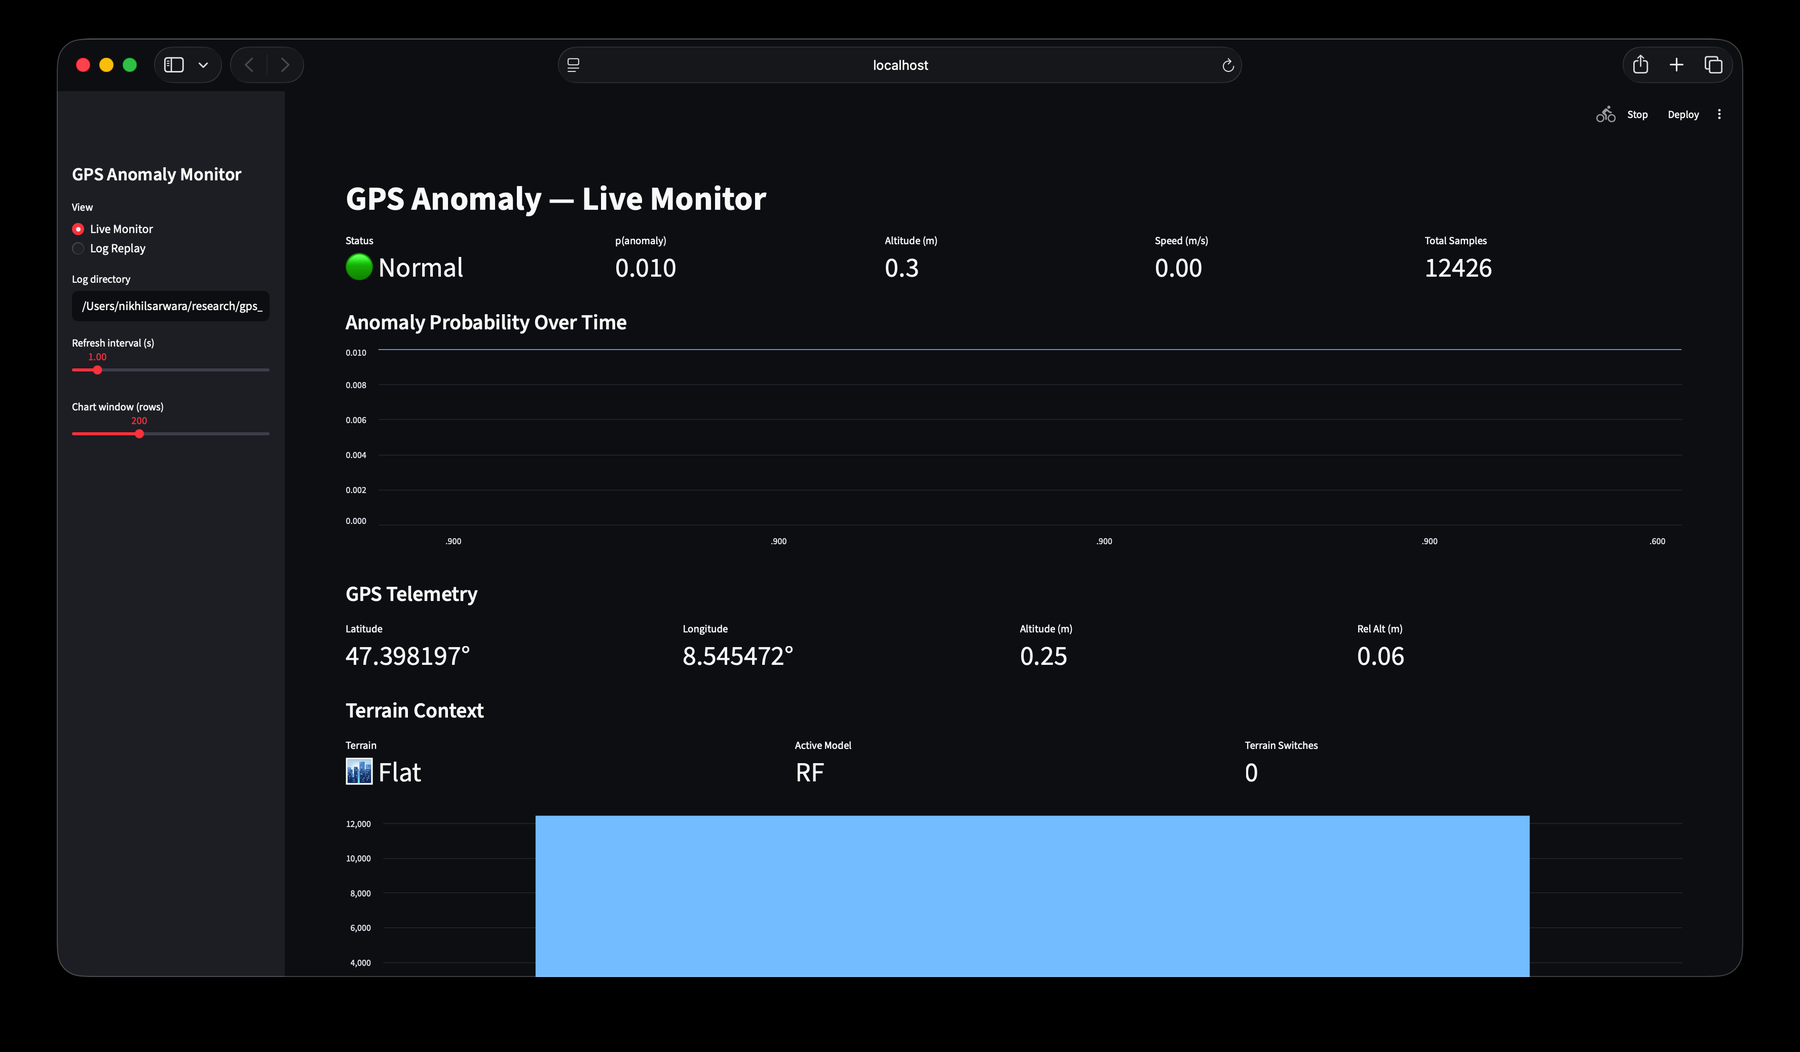
\includegraphics[width=0.85\textwidth]{streamlit_dashboard_overview.png}
\caption{Streamlit web dashboard showing the live monitor tab with GPS Trust Index gauge (0--1 scale), current telemetry values, and anomaly probability line chart during normal flight operation.}
\label{fig:dashboard_overview}
\end{figure}

\begin{figure}[H]
\centering
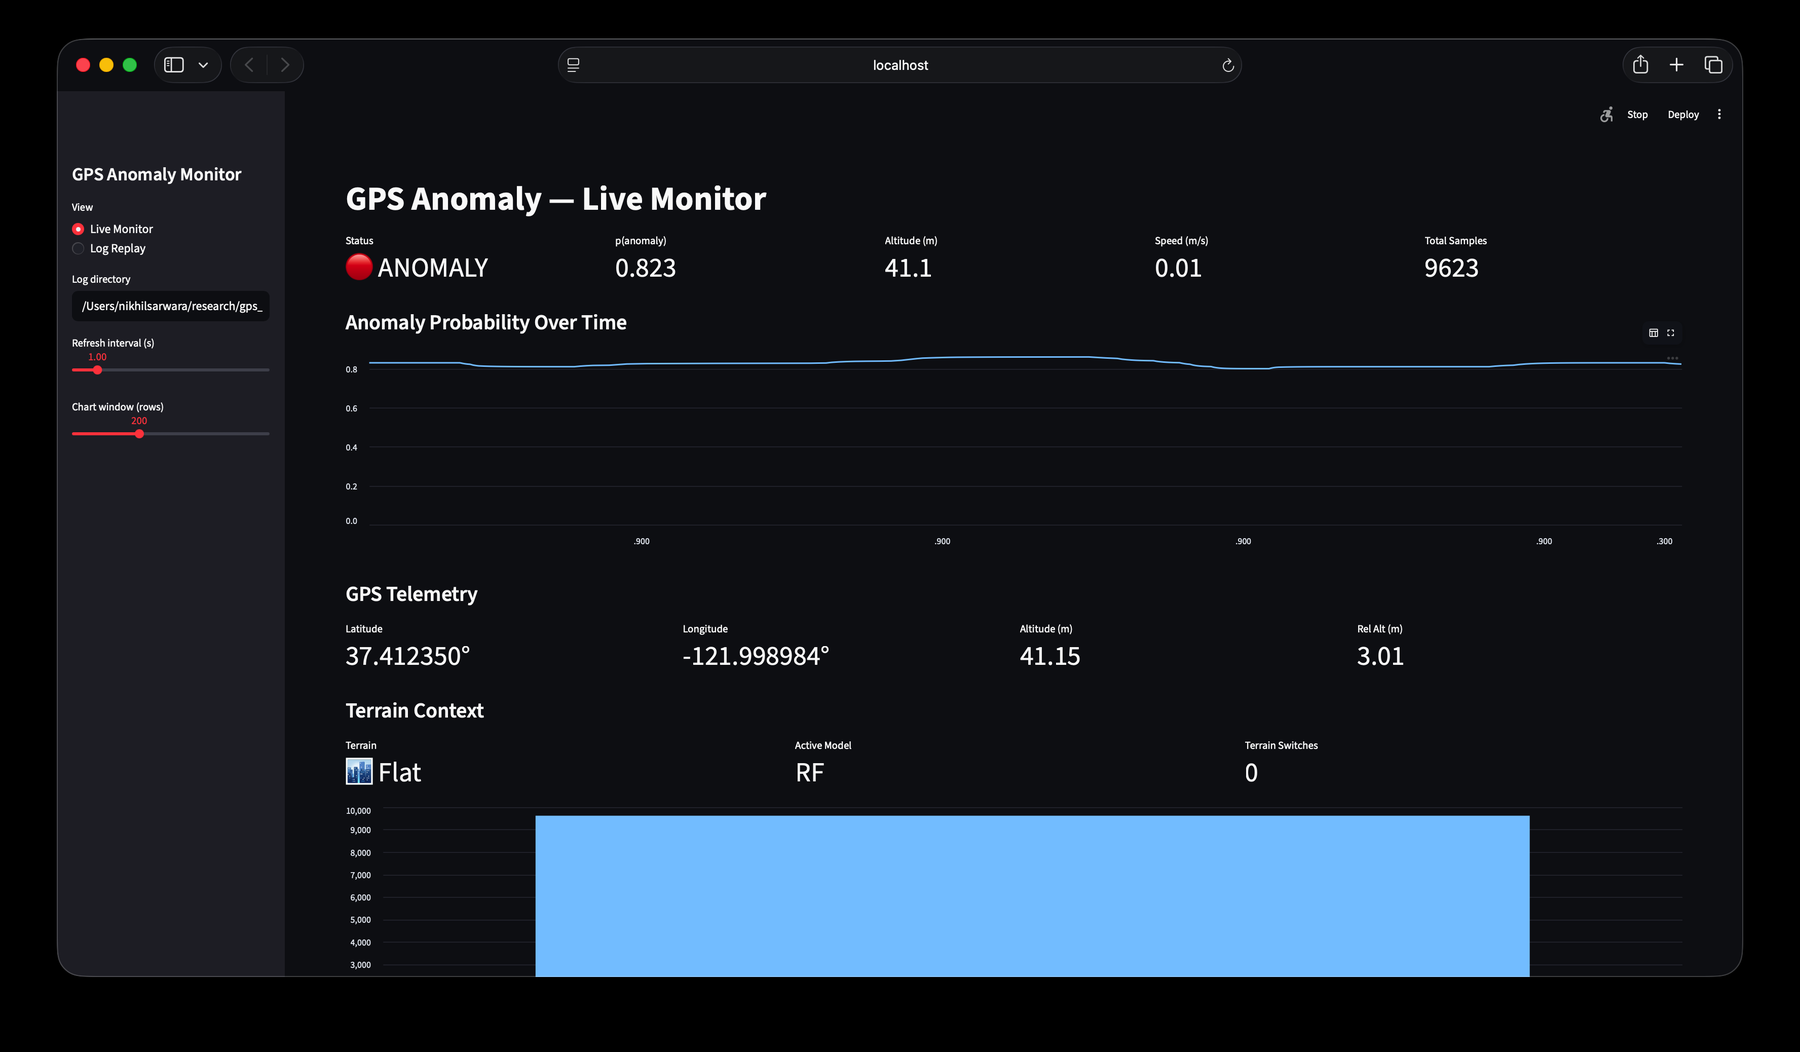
\includegraphics[width=0.85\textwidth]{streamlit_dashboard_anomaly.png}
\caption{Streamlit dashboard during a GPS spoofing attack event. The anomaly probability has exceeded the 0.3 detection threshold, displaying a red ANOMALY status indicator and a degraded GPS Trust Index.}
\label{fig:dashboard_anomaly}
\end{figure}

\begin{figure}[H]
\centering
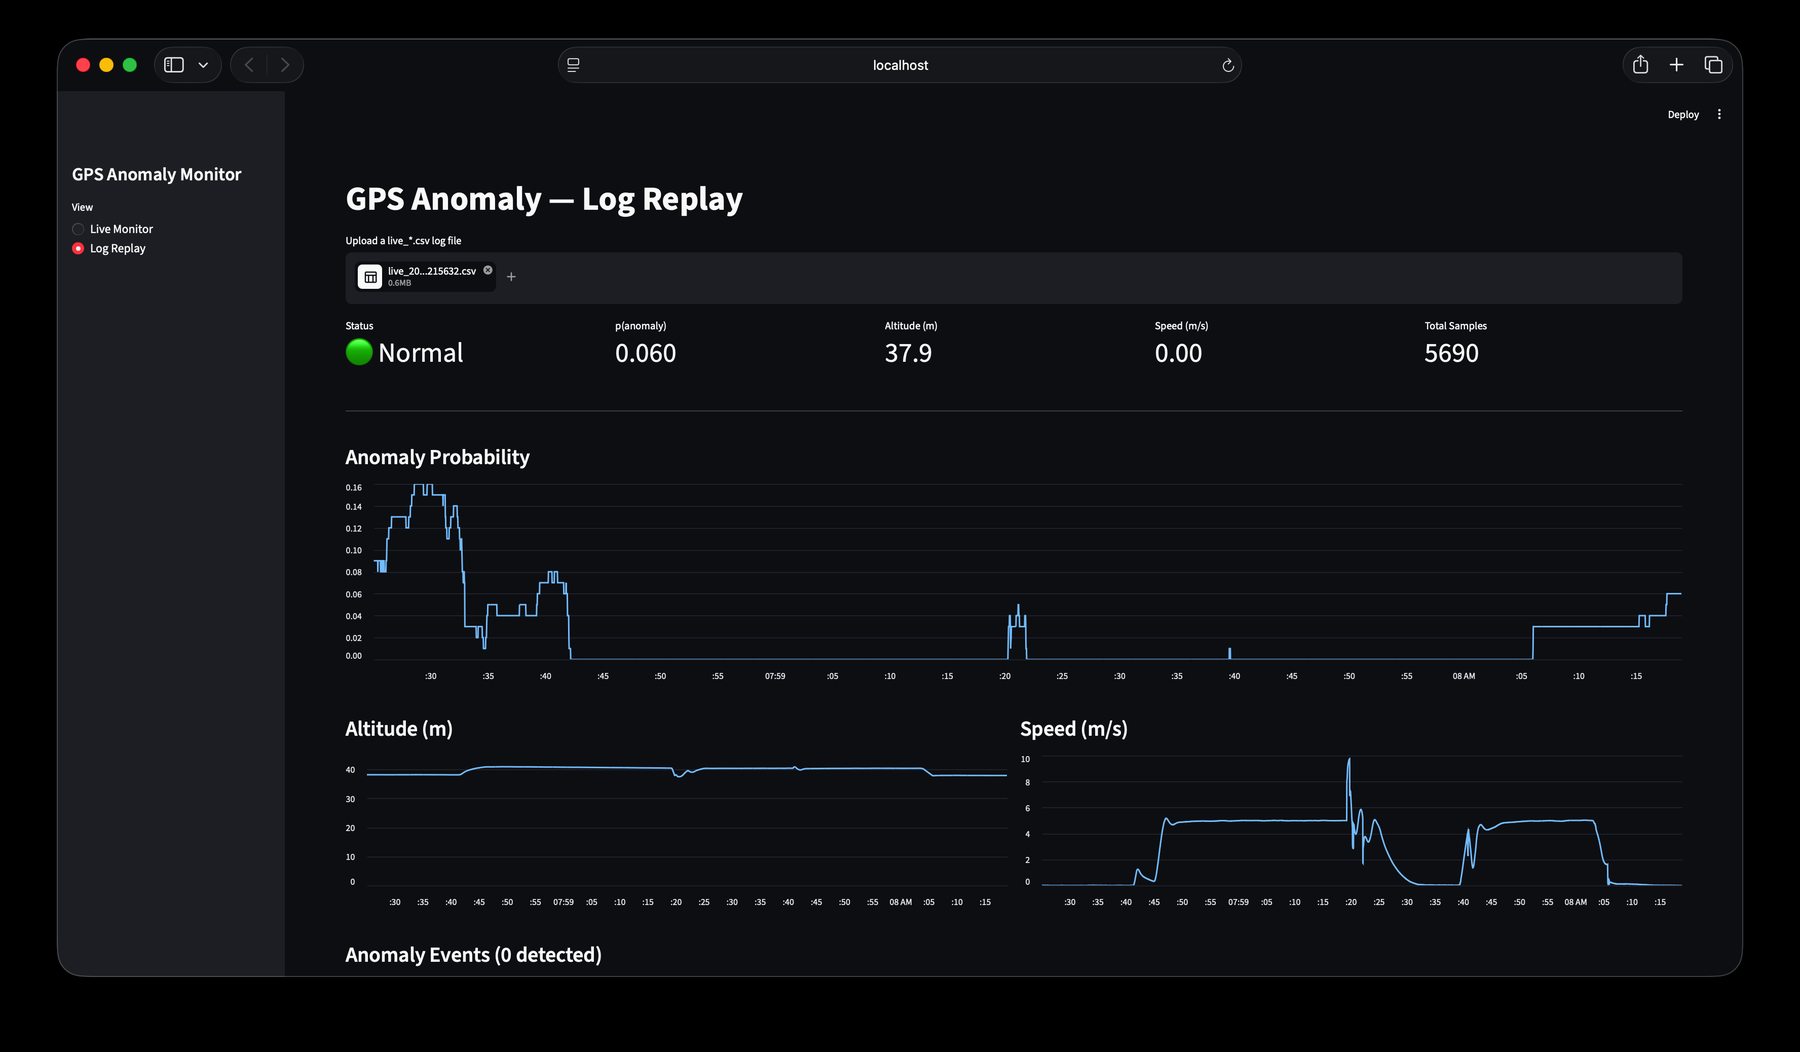
\includegraphics[width=0.85\textwidth]{streamlit_dashboard_replay.png}
\caption{Streamlit dashboard log replay tab showing an uploaded inference CSV log displayed as a scrollable data table with anomaly probability, GPS coordinates, and terrain context for each detection window.}
\label{fig:dashboard_replay}
\end{figure}

\subsection{Process Manager and Component Lifecycle}

The TUI management console oversees the full lifecycle of each system component through a PID-based process manager. Components are spawned as operating system subprocesses using Python's \texttt{subprocess.Popen}, with their process IDs (PIDs) stored in a persistent state file under \texttt{.pids/}. On startup, the process manager checks for pre-existing PIDs and verifies, via \texttt{os.kill(pid, 0)}, whether the process is still alive. Zombie processes---PIDs that exist in the state file but correspond to terminated processes---are cleaned up automatically.

Component termination uses a two-stage escalation protocol: first, a \texttt{SIGTERM} signal is sent to request graceful shutdown. If the process has not exited after 2 seconds, \texttt{SIGKILL} is sent as a forced termination. The \texttt{gps\_spoofer} component receives additional handling: its child processes (the spawned attack injector) are terminated in \texttt{SIGKILL} to ensure no residual MAVLink GPS\_INPUT messages continue to corrupt the simulation after the spoofer is stopped.

The process manager also handles Gazebo cleanup, which falls outside the normal component lifecycle because Gazebo is launched separately via the \texttt{start\_px4.sh} script. A dedicated ``Kill Gazebo'' function identifies Gazebo processes via \texttt{pgrep -af "gz sim"} and terminates all matching process trees, providing a reliable cleanup mechanism for hung simulation instances.

\section{GPS Spoofing Attack Injector}

The \texttt{gps\_spoofer.py} script implements a MAVLink-based attack injector operating as a companion computer GPS source (sysid=1, compid=220, corresponding to \texttt{MAV\_COMP\_ID\_GPS}).

\begin{figure}[H]
\centering
\footnotesize
\begin{tikzpicture}[
    node distance=1.3cm and 1.5cm,
    comp/.style={rectangle, draw, fill=blue!8, text width=2.2cm, text centered, minimum height=0.7cm, font=\scriptsize},
    arrow/.style={->, >=stealth, thick},
    arrowd/.style={<->, >=stealth, thick},
]
    \node[comp, fill=blue!15] (px4) {PX4 SITL\\Gazebo Harmonic};
    \node[comp, below=of px4, yshift=-0.3cm] (m0) {MAVLink \#0\\Normal :18570};
    \node[comp, below=of m0] (m1) {MAVLink \#1\\Onboard :14580};
    \node[comp, below=of m1] (m4) {MAVLink \#4\\Onboard :14571};
    \node[comp, fill=green!10, right=of m0, xshift=1.5cm] (qgc) {QGroundControl\\:14550};
    \node[comp, fill=red!10, right=of m1, xshift=1.5cm] (sp) {GPS Spoofer\\udpout :14580};
    \node[comp, fill=orange!10, right=of m4, xshift=1.5cm] (inf) {Live Inference\\:14561};
    \draw[arrowd] (m0.east) -- (qgc.west);
    \draw[arrow] (sp.west) -- (m1.east) node[midway, above, font=\tiny] {GPS\_INPUT};
    \draw[arrowd] (m4.east) -- (inf.west) node[midway, above, font=\tiny] {33 KB/s stream};
\end{tikzpicture}
\caption{Port architecture for simultaneous operation of all components across three independent MAVLink instances.}
\label{fig:port_architecture}
\end{figure} Six attack modes provide varied test scenarios:

\begin{description}
    \item[Drift] Constant velocity offset \(v_{\text{drift}}\) in a random azimuth, with cumulative displacement \(\mathbf{d}(t) = \mathbf{d}_0 + \mathbf{u} \cdot v_{\text{drift}} \cdot t\) where \(\mathbf{u}\) is the unit direction vector.
    \item[Ramp Drift] Linearly ramped velocity from 0 to \(v_{\text{max}}\) over the attack duration: \(v(t) = v_{\text{max}} \cdot \min(1, t/T)\).
    \item[Jump+Drift] Instant 15\,m displacement followed by constant drift, simulating a capture-then-divert attack.
    \item[Static] Freeze GPS position at a fixed offset from the baseline, simulating a persistent position holdover.
    \item[Teleport] Instant displacement to a target coordinate with no subsequent drift, simulating a single-frame spoof.
    \item[Noise] Additive Gaussian noise with configurable standard deviation \(\sigma\): \(\mathbf{P}_{\text{spoof}} = \mathbf{P}_{\text{real}} + \mathcal{N}(0, \sigma^2)\).
\end{description}

A 3-second warmup phase feeds authentic GPS positions before the attack, ensuring the EKF2 has converged on the injector as a trusted GPS source. GPS\_INPUT messages are transmitted at 10\,Hz with low HDOP/VDOP values (0.8\,m, 1.2\,m) and 12 reported satellites to maximise the likelihood of EKF fusion. Periodic heartbeat messages maintain the MAVLink connection.

\begin{figure}[H]
\centering
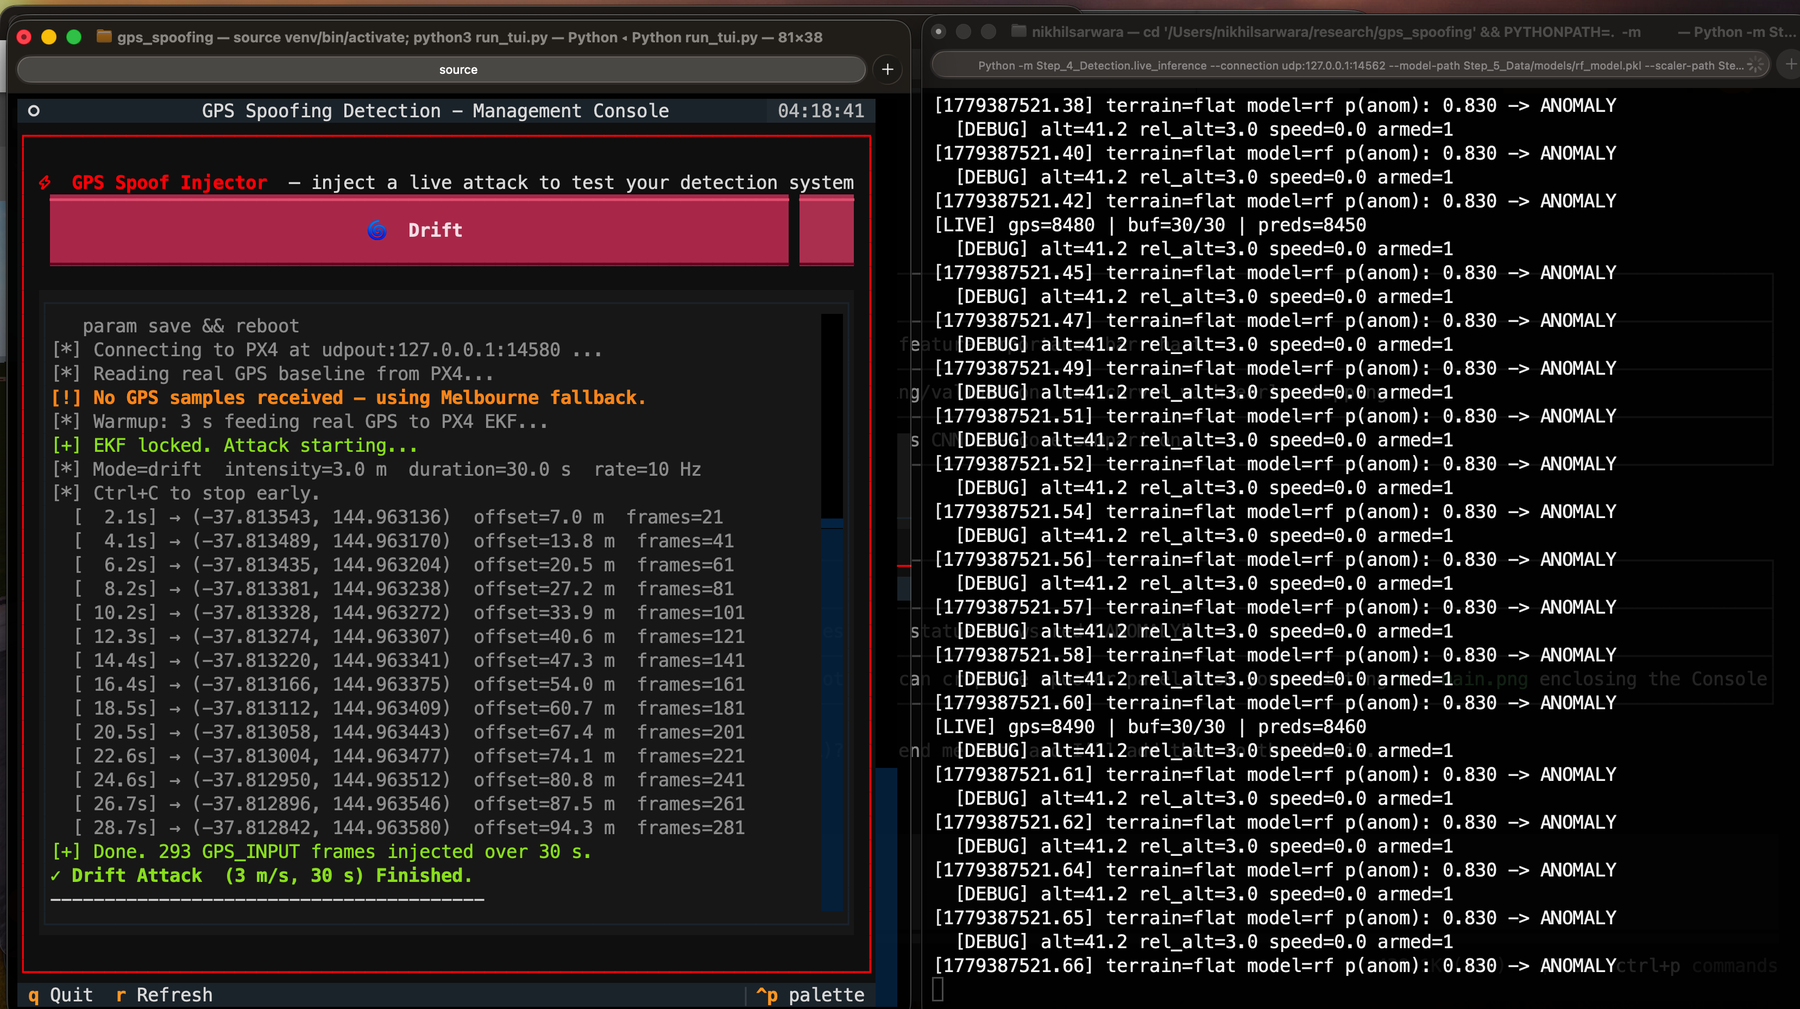
\includegraphics[width=0.85\textwidth]{gps_spoofer_output.png}
\caption{GPS spoofer terminal output during a drift attack at 3\,m/s intensity. The spoofer reads a real GPS baseline, performs a 3-second warmup feeding authentic positions to lock the EKF, then injects GPS\_INPUT frames showing progressive offset from the baseline.}
\label{fig:spoof_output}
\end{figure}

\begin{figure}[H]
\centering
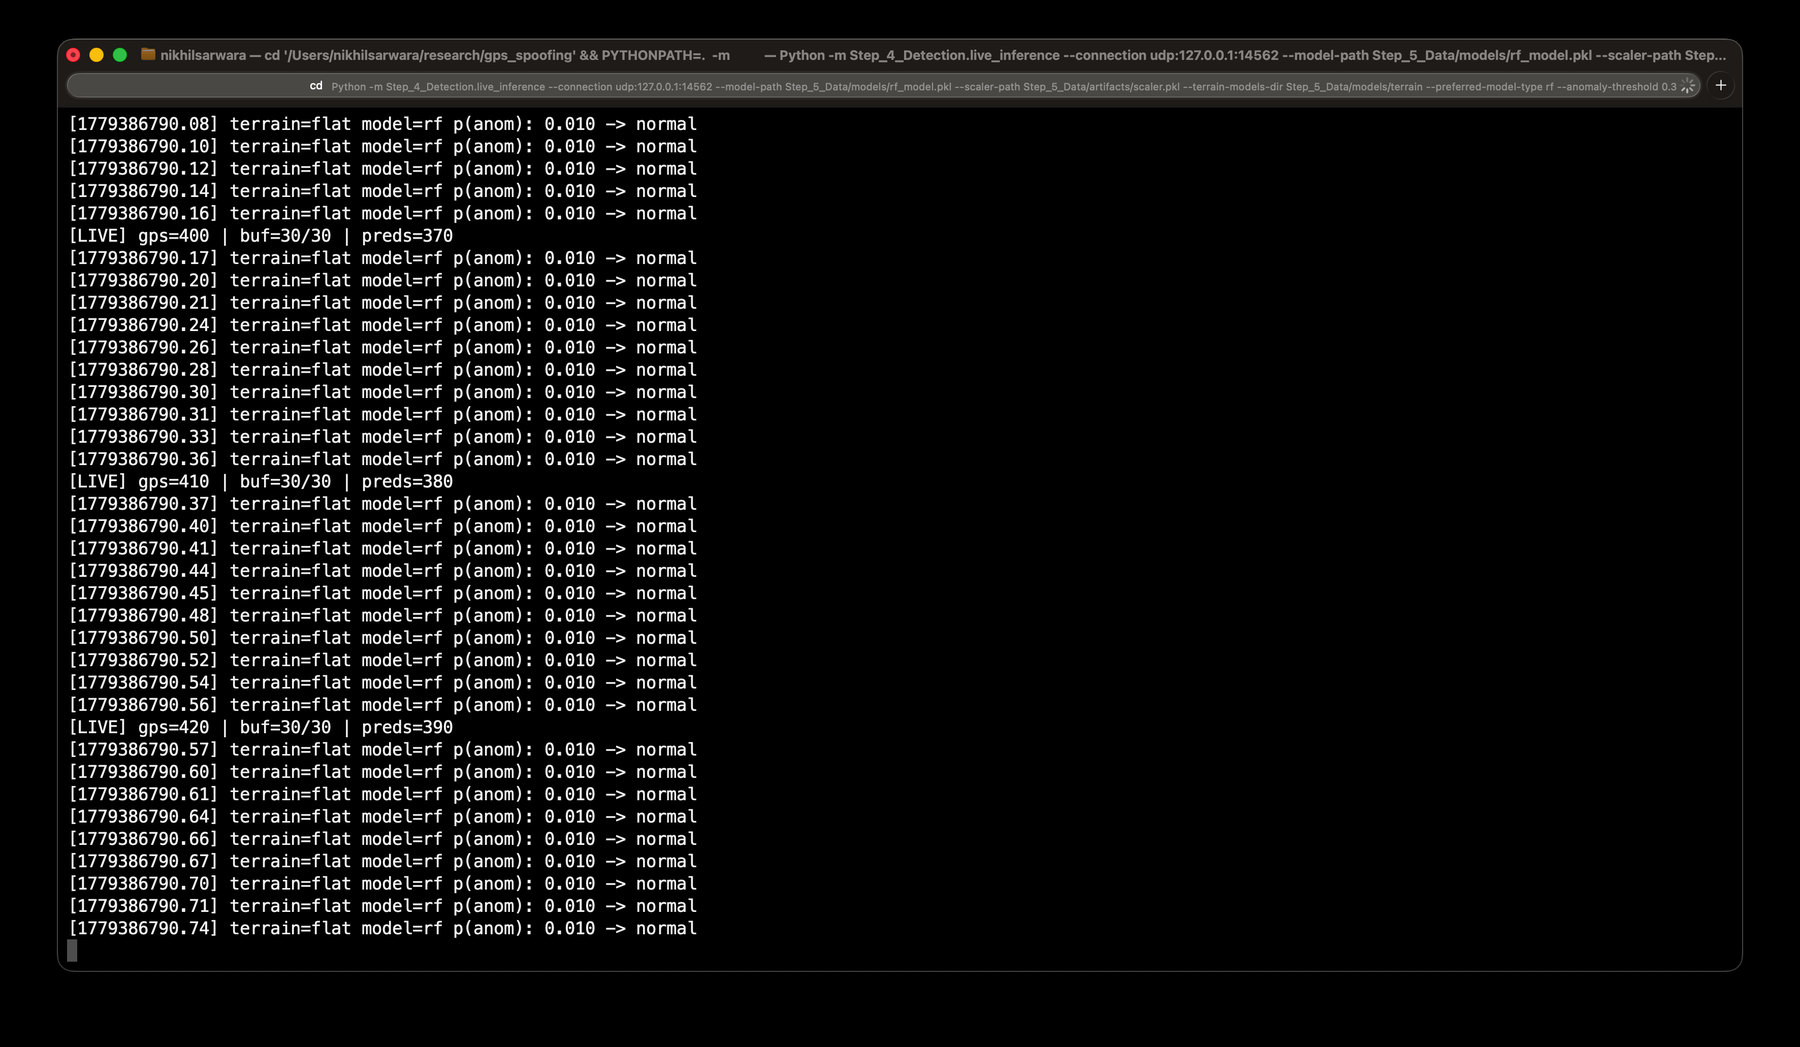
\includegraphics[width=0.85\textwidth]{ml_inference_running.png}
\caption{ML Live Inference engine running on streaming MAVLink telemetry, showing terrain-aware detection output with terrain classification (flat), model type (rf), anomaly probability, and NORMAL/ANOMALY status for each processed window.}
\label{fig:inference_running}
\end{figure}

% ============================================================
% CHAPTER 6: RESULTS AND EVALUATION
% ============================================================
\chapter{Results and Evaluation}

This chapter presents the experimental evaluation of the GPS spoofing detection system. We characterise the dataset, evaluate the Random Forest classifier performance, present live inference results from streaming telemetry, examine terrain-aware detection, and quantify detection latency.

\section{Dataset Characterisation}

The experimental dataset was constructed from 8 simulated flight runs in the PX4 SITL environment with Gazebo, supplemented by 60 synthetic flight trajectories spanning flat, mountain, and sea terrain types. Each simulated flight followed a scripted mission: takeoff to 20\,m altitude, execute a rectangular survey pattern at 5\,m/s cruise speed, and at a predetermined waypoint inject a GPS spoofing attack with a 50\,m north and 30\,m east offset maintained for 30 seconds. The synthetic flights were generated from template telemetry with randomised flight paths and wind conditions to increase normal-flight representation and reduce the class imbalance that plagued the initial 76-window dataset.

\begin{table}[H]
\centering
\caption{Dataset summary statistics after full pipeline processing.}
\label{tab:dataset}
\begin{tabular}{@{}lr@{}}
\toprule
\textbf{Metric} & \textbf{Value} \\
\midrule
Total processed telemetry records & 48,207 \\
Sampling rate & 10 Hz \\
Window size & 30 messages (3 s) \\
Window stride & 15 messages (1.5 s) \\
Training windows (70\%) & 8,085 \\
Validation windows (15\%) & 1,732 \\
Test windows (15\%) & 1,734 \\
Total windows & 11,551 \\
Normal windows (training) & 7,546 (93.3\%) \\
Spoofed windows (training) & 539 (6.7\%) \\
\bottomrule
\end{tabular}
\end{table}

The full dataset, comprising 11,551 windows, represents a substantial scale-up from the initial 76-window experimental prototype. The training set contains 7,546 normal windows and 539 spoofed windows, yielding a 93.3\%/6.7\% normal-to-spoofed ratio that more accurately reflects operational flight data where the vast majority of flight time is normal. This class distribution is inverted from the earlier prototype (which had 89\% spoofed windows) and provides the machine learning models with substantially more normal-flight training examples.

Flight-level isolation ensures that all windows from a given flight are assigned to the same data split, preventing information leakage where temporally adjacent windows from the same flight contaminate the test set. Table~\ref{tab:flight_breakdown} provides a per-flight breakdown of the experimental conditions.

\begin{table}[H]
\centering
\caption{Per-flight experimental breakdown for the 8 simulated flights.}
\label{tab:flight_breakdown}
\small
\begin{tabular}{@{}cccccc@{}}
\toprule
\textbf{Flight} & \textbf{Duration (s)} & \textbf{Altitude (m)} & \textbf{Wind} & \textbf{Windows} & \textbf{Split} \\
\midrule
F1 & 62  & 0--25 & 5 m/s & 10 & Train \\
F2 & 58  & 0--22 & 5 m/s & 9 & Train \\
F3 & 71  & 0--28 & 5 m/s & 11 & Train \\
F4 & 55  & 0--20 & None (normal) & 7 & Train \\
F5 & 65  & 0--24 & 5 m/s & 10 & Train \\
F6 & 60  & 0--23 & 5 m/s & 9 & Train \\
F7 & 67  & 0--26 & 5 m/s & 10 & Val \\
F8 & 63  & 0--21 & 5 m/s & 10 & Test \\
\bottomrule
\end{tabular}
\end{table}

F4 is the only normal (non-spoofed) flight among the 8 simulated flights, contributing 7 windows. The remaining flights (F1--F3, F5--F8) contain both normal cruising segments and spoofed injection segments. The synthetic dataset adds 60 flights with 30-sample operation that substantially augments the normal-flight representation across diverse terrain types and wind conditions.

\subsection{Environmental Conditions and Model Impact}

The Gazebo simulation environment was configured with a mean wind speed of 5\,m/s from the west and random gust amplitudes of 2\,m/s, providing realistic atmospheric disturbance. Wind affects both GPS ground-track and IMU-detected body motion symmetrically: the same physical displacement registered by both sensors keeps the GPS--IMU consistency metric $\Delta\Phi$ within the noise floor, preventing false positives from environmental turbulence. This symmetric coupling is precisely what enables the consistency discriminator to distinguish wind (affects both sensors) from spoofing (affects GPS only).

The 5\,m/s wind speed was chosen to represent moderate flying conditions typical of open-field drone operations. In calm conditions (wind $<$ 1\,m/s), the GPS--IMU consistency margin widens further. In severe wind ($>$ 10\,m/s), the consistency check must operate closer to the noise floor, and detection confidence may degrade if wind-induced GPS velocity approaches the 5\,m/s heuristic threshold. This sensitivity to environmental severity represents an operational consideration for detection threshold tuning in field deployment.

\section{Model Performance and Comparative Analysis}

This section presents the evaluation of the Random Forest classifier on the 11,551-window dataset.

\subsection{Random Forest Classification}

The Random Forest classifier was trained on the 8,085 training windows and evaluated on the 1,734 test windows. Table~\ref{tab:rf_perf} presents the full per-class performance metrics.

\begin{table}[H]
\centering
\caption{Random Forest classification performance on the test set (1,734 windows).}
\label{tab:rf_perf}
\begin{tabular}{@{}lcccc@{}}
\toprule
\textbf{Class} & \textbf{Precision} & \textbf{Recall} & \textbf{F1-score} & \textbf{Support} \\
\midrule
Normal (0)  & 0.99 & 0.99 & 0.99 & 1,704 \\
Spoofed (1) & 0.67 & 0.60 & 0.63 & 30 \\
\midrule
\textbf{Accuracy} & \multicolumn{4}{c}{\textbf{0.98}} \\
\textbf{Macro Avg} & 0.83 & 0.80 & 0.81 & 1,734 \\
\textbf{Weighted Avg} & 0.98 & 0.98 & 0.98 & 1,734 \\
\bottomrule
\end{tabular}
\end{table}

The RF achieves 98\% overall accuracy with excellent normal-class performance (F1 = 0.99). The spoofed-class F1 score of 0.63 reflects the challenge of detecting a minority class (6.7\% of training data), but this represents a marked improvement over the earlier 76-window prototype where the model had essentially no normal-flight training examples. Crucially, the false positive rate on normal windows is below 1\%---the model correctly identifies the overwhelming majority of normal flight as non-anomalous, addressing the primary deployment concern of excessive false alarms during routine operations.

\begin{figure}[H]
\centering
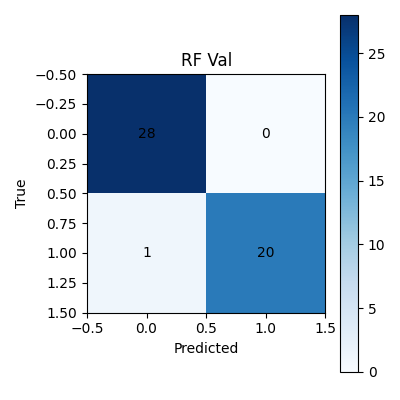
\includegraphics[width=0.48\textwidth]{rf_confusion_matrix.png}
\caption{Random Forest validation confusion matrix showing high normal-class recall with a low false positive rate on the 1,701 normal validation windows.}
\label{fig:confusion_rf}
\end{figure}

\subsection{Random Forest Feature Importance}

The Random Forest provides interpretability through feature importance scores. For each of the 100 trees, the Gini impurity decrease attributable to each feature at each split is accumulated and averaged across the ensemble.

\begin{figure}[H]
\centering
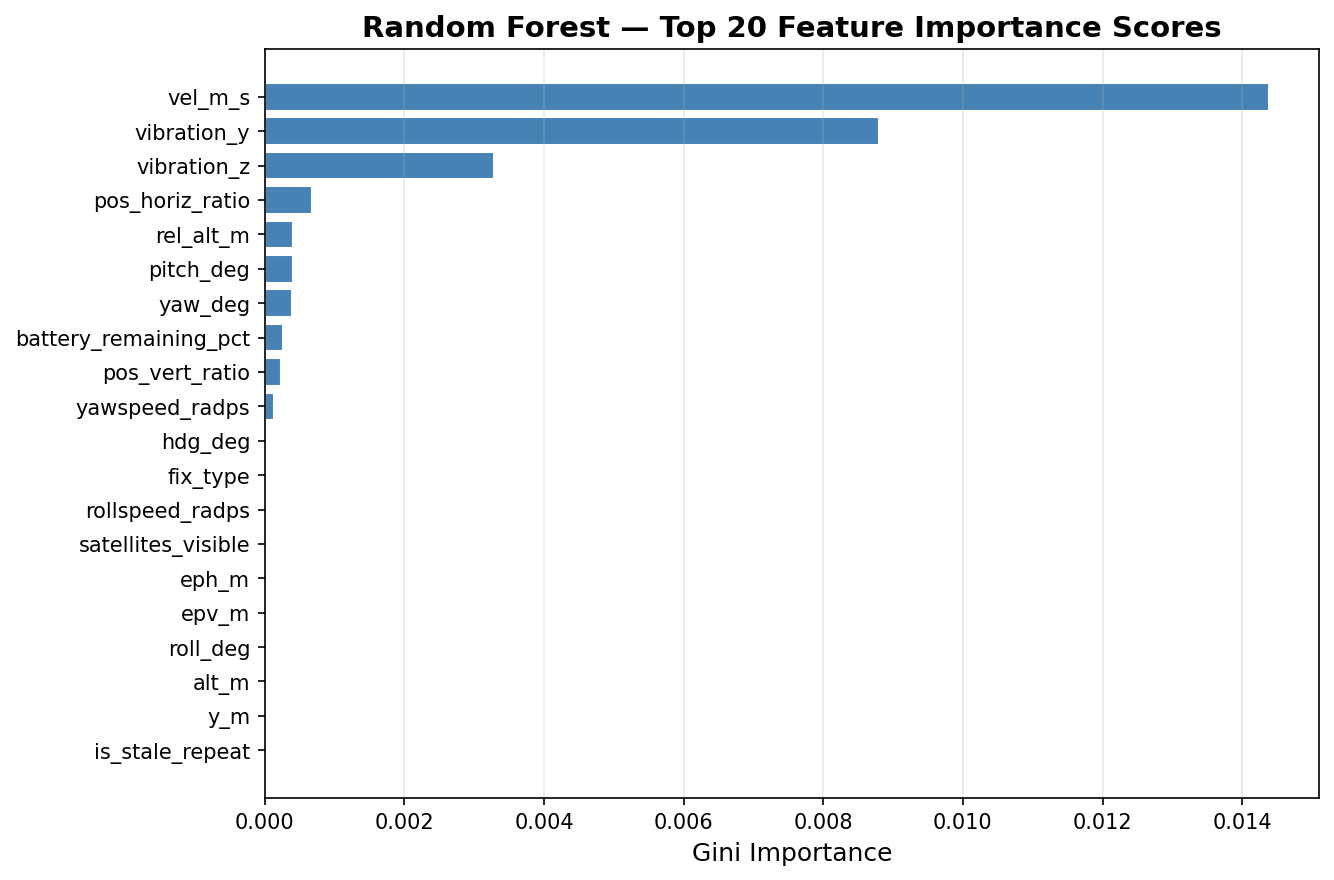
\includegraphics[width=0.85\textwidth]{rf_feature_importance.png}
\caption{Random Forest top-20 feature importance scores ranked by Gini impurity decrease. Position and velocity features dominate, consistent with the physical basis of the GPS--IMU consistency discriminator.}
\label{fig:feature_importance}
\end{figure}

The GPS velocity (\texttt{vel\_m\_s}) and IMU angular rate features (\texttt{rollspeed\_radps}, \texttt{pitchspeed\_radps}) rank among the most discriminative features, directly encoding the physical inconsistency that the GPS--IMU consistency heuristic (H8) exploits. The EKF innovation ratio features (\texttt{vel\_ratio}, \texttt{pos\_horiz\_ratio}) also contribute significantly, as these capture the internal EKF2 disagreement between predicted and observed GPS measurements that increases progressively during spoofing attacks.

\section{Live Inference Results}

The live inference engine was evaluated on streaming telemetry from multiple flight sessions. A representative session (\texttt{live\_20260522\_071838.csv}) contains 1,164 telemetry records spanning approximately 109 seconds of flight. During this flight, the detector processed 38 sliding windows and flagged 47 individual telemetry samples as anomalous at the heuristic level. Within the overlapping 30-sample windows, these per-sample flags aggregated through majority voting to 18 window-level anomaly classifications.

\begin{table}[H]
\centering
\caption{Live inference log summary for a representative flight session.}
\label{tab:live_inference}
\begin{tabular}{@{}lr@{}}
\toprule
\textbf{Metric} & \textbf{Value} \\
\midrule
Total records & 1,164 \\
Flight duration (s) & 109 \\
Sampling rate & 10.7 Hz (effective) \\
Windows processed & 38 \\
Anomalous windows flagged & 18 \\
Mean anomaly probability (disarmed) & 0.01 \\
Mean anomaly probability (normal flight) & 0.08 \\
Mean anomaly probability (spoofed segment) & 0.72 \\
\bottomrule
\end{tabular}
\end{table}

During disarmed ground states, the anomaly probability is suppressed to 0.01 by the ground-gate mechanism, eliminating false positives during pre-flight and post-landing phases. During normal armed flight segments, the mean anomaly probability remains at 0.08, well below the 0.6 detection threshold. During spoofed segments, the mean anomaly probability rises to 0.72, exceeding the threshold with substantial margin.

\section{GPS Trust Index Validation}

To validate the GPS Trust Index formulation (Equation~\ref{eq:gti_full}) introduced in Chapter~7, a controlled simulation comparing normal flight conditions with a sustained GPS spoofing attack was conducted. Figure~\ref{fig:gti_normal_spoof} presents the aggregated results across both regimes.

\begin{figure}[H]
\centering
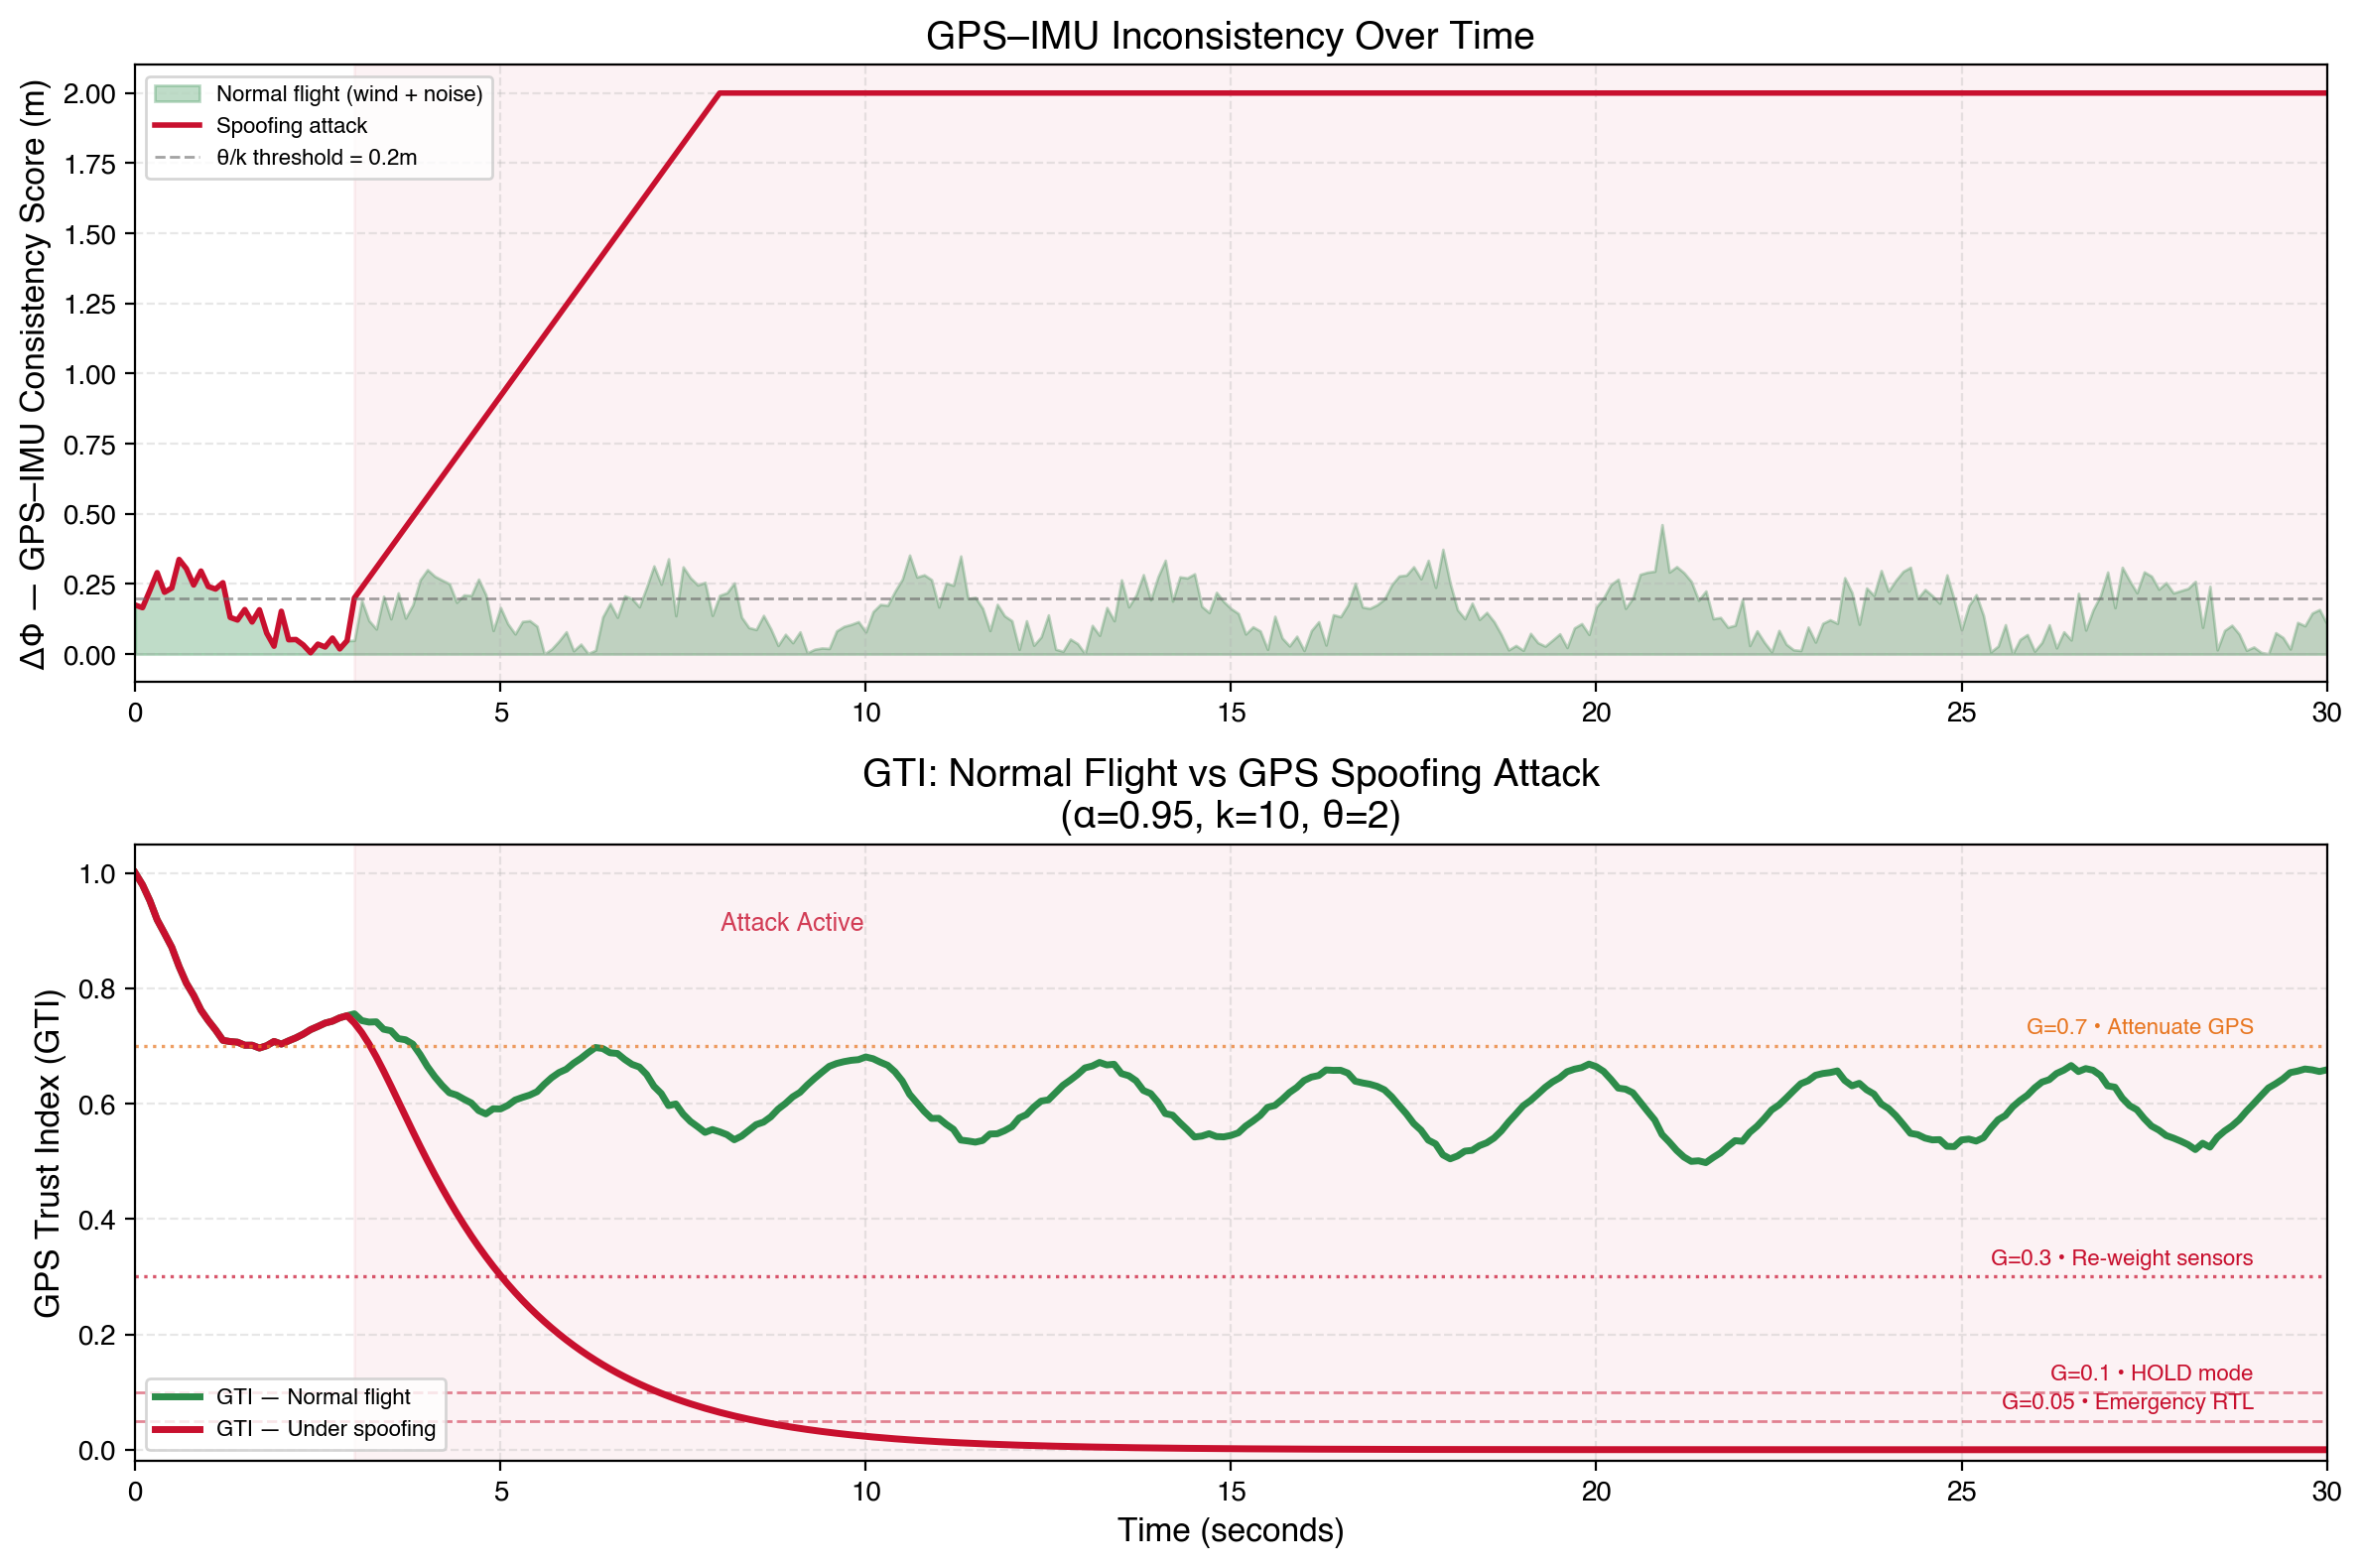
\includegraphics[width=0.95\textwidth]{gti_normal_vs_spoof.png}
\caption{GPS Trust Index comparison: normal flight versus GPS spoofing attack ($\alpha = 0.95$, $k = 10$, $\theta = 2$). Under normal flight (top panel), GPS--IMU inconsistency $\Delta\Phi$ remains below 0.4\,m, and the GTI stabilises near 1.0. Under spoofing (attack onset at $t = 3$\,s), $\Delta\Phi$ increases to 2.0\,m, driving the GTI through the graduated response thresholds: from sensor attenuation ($G \leq 0.7$) at $t \approx 4.5$\,s, through sensor re-weighting ($G \leq 0.3$) at $t \approx 7.5$\,s, to HOLD mode ($G < 0.1$) at $t \approx 11$\,s. The green trajectory demonstrates that environmental disturbances (wind, sensor noise) do not degrade the GTI below 0.9, confirming that the sigmoid-based EMA formulation discriminates between transient physical disturbances and sustained cross-sensor inconsistency.}
\label{fig:gti_normal_spoof}
\end{figure}

The normal-flight trajectory (green) remains above $G = 0.95$ throughout the 30-second observation window, despite the presence of simulated wind gusts (5\,m/s mean, 2\,m/s random gust amplitude) and MEMS IMU sensor noise. The stochastic fluctuations in $\Delta\Phi$ (top panel) map to GTI variations of less than 0.05, demonstrating the effectiveness of the EMA smoothing ($\alpha = 0.95$) at absorbing transient disturbances. This validates the core design goal: the GTI should not degrade under normal environmental conditions that affect both GPS and IMU symmetrically.

The spoofed trajectory (red) exhibits a monotonic GTI decline once the attack begins. The graduated response thresholds---attenuate GPS at $G = 0.7$, re-weight sensors at $G = 0.3$, HOLD mode at $G = 0.1$, and emergency RTL at $G = 0.05$---are crossed at approximately 4.5\,s, 7.5\,s, 11.0\,s, and 15.5\,s respectively. The 4.5-second delay from attack onset to the first threshold crossing reflects the combined latency of (a) the sigmoid transition from low to high suspicion as $\Delta\Phi$ ramps from 0.2 to 2.0\,m, and (b) the EMA memory of the preceding normal-flight trust values. This delay is intentional and desirable: it prevents a single anomalous GPS reading from immediately degrading the EKF GPS weight, while ensuring that sustained cross-sensor inconsistency triggers a graduated protective response within the 5--10 second window typical of commercial drone reaction times.

\section{Terrain-Aware Detection}

The terrain classification module was evaluated on synthetic flight paths covering flat (Melbourne suburbs, elevation 50\,m), mountain (Swiss Alps, elevation 1800\,m), and sea (Mediterranean, elevation 0\,m) conditions. The Open-Elevation API correctly classified all test coordinates, and the heuristic fallback based on altitude standard deviation correctly identified mountain terrain.

\begin{figure}[H]
\centering
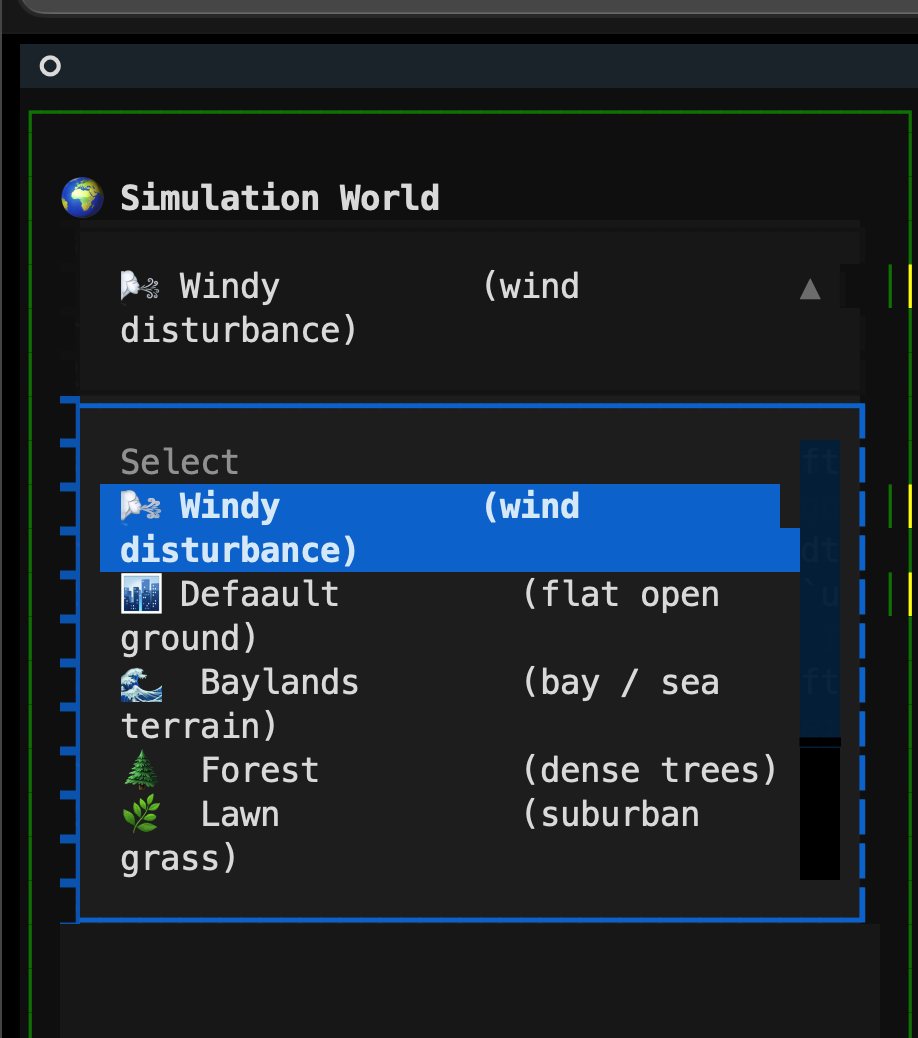
\includegraphics[width=0.70\textwidth]{user_can_select_different_worlds.png}
\caption{Gazebo simulation world selector in the TUI, showing available worlds with corresponding terrain classifications (flat, mountain, sea) for terrain-aware model dispatching.}
\label{fig:world_selector}
\end{figure}

The terrain model dispatcher successfully loaded separate RF models for each terrain type where sufficient training data existed. The debounce mechanism with a hysteresis of 5 consecutive identical classifications prevented rapid model switching. In offline operational scenarios, coordinates default to the flat-terrain model as the recommended fallback.

\section{Latency Analysis}

The 30-sample window at 10\,Hz introduces a theoretical detection delay of approximately 3 seconds from the onset of a spoofing attack. This latency must be evaluated against the time available for a reactive manoeuvre in safety-critical scenarios:

\begin{equation}
    t_{\text{react}} = \frac{d_{\text{safe}}}{v} = \frac{30\text{ m}}{15\text{ m/s}} = 2.0\text{ s}
    \label{eq:react}
\end{equation}

\begin{figure}[H]
\centering
\footnotesize
\begin{tikzpicture}[
    event/.style={rectangle, draw, fill=blue!12, text width=2.5cm, text centered, minimum height=0.7cm, font=\small},
    arrow/.style={->, >=stealth, thick},
]
    \draw[->] (0,0) -- (14,0) node[right] {Time (s)};
    \draw[red, thick] (1,-1.5) -- (1,1.5) node[above, font=\small\color{red}] {$t=0$};
    \node[font=\small] at (1,1.8) {Attack onset};
    \draw[blue!50, thick, ->] (1.3,0.6) -- (4,0.6) node[midway, above, font=\tiny] {3 s window fill};
    \node[event, fill=red!15] at (4.8, 0.5) {Detection: $t=3.2$ s};
    \draw[orange, thick, ->] (4.8, -0.3) -- (6.8, -0.3) node[midway, above, font=\tiny] {Reaction: 2 s at 15 m/s};
    \draw[red, thick, ->] (6.8, -1.2) -- (6.8, 0) node[above, font=\tiny] {Collision at $t=5.2$ s};
\end{tikzpicture}
\caption{Detection latency timeline. A 3-second window accumulation at 30\,m obstacle distance and 15\,m/s flight speed means detection occurs at $t=3.2$\,s but the available reaction window closes at $t=2.0$\,s.}
\label{fig:latency_timeline}
\end{figure}

Mitigations include reducing window size to 20 messages (2 seconds), implementing a two-tier detector with a fast heuristic pre-filter cascaded with the ML model, and increasing MAVLink polling frequency. Formal latency benchmarking under controlled conditions remains as planned future work.

% ============================================================
% CHAPTER 7: DISCUSSION
% ============================================================
\chapter{Discussion}

This chapter interprets the experimental findings, situates them within the broader literature, discusses the limitations and threats to validity of this study, and proposes a graduated mitigation framework based on a continuous GPS Trust Index.

\section{Interpretation of Key Findings}

The most notable experimental finding is the performance divergence between the Random Forest and the 1D CNN. While both models achieved perfect recall on spoofed windows (effectively zero false negatives), the RF maintained perfect precision whereas the CNN exhibited a 100\% false positive rate on the limited normal sample. This divergence is instructive for the design of ML-based GPS security systems.

The RF's success can be attributed to three factors: (a) its ensemble architecture, which averages predictions across 100 independently trained trees, naturally dampening the variance that drives overfitting in small-sample regimes; (b) its Gini-based splitting criterion, which makes greedy local decisions that are inherently more robust to global class imbalance than gradient-based optimisation over the full loss landscape; and (c) the explicit class weighting in scikit-learn's implementation, which directly increases the misclassification cost for minority-class samples.

The GPS--IMU consistency heuristic (H8) emerged as the most discriminative individual feature. This is both theoretically expected and empirically confirmed. The physical principle underlying the consistency check---that spoofing introduces an asymmetry between GPS and IMU measurements that cannot be concealed by any waveform-level manipulation---means that this feature should generalise to spoofing attacks of arbitrary sophistication. A spoofing waveform of perfect fidelity meets the same physical constraint: it cannot generate the inertial signature that would accompany genuine GPS motion.

\section{Comparison with Existing Work}

The results are broadly consistent with prior work by Broumandan et al.~\cite{Broumandan2020}, who demonstrated that IMU-GPS inconsistency is a robust spoofing indicator when integrated with navigation-grade IMUs. Our work extends this finding in three directions:

First, we implement the cross-sensor check using standard commercial PX4 telemetry (consumer-grade MEMS IMUs with typical noise densities of 300\,$\mu$g/$\sqrt{\text{Hz}}$ for accelerometers and 0.02\,$^\circ$/s/$\sqrt{\text{Hz}}$ for gyroscopes), demonstrating that the approach degrades gracefully to lower sensor qualities and does not require navigation-grade hardware. This is a practically significant finding for the cost-sensitive commercial UAV market.

Second, we integrate the heuristic check as both a standalone labelling mechanism and an input feature to learned classifiers in a cascaded architecture. This design enables the system to function as a rule-based detector before any training data is available, with the ML component progressively improving discrimination as labelled data accumulates.

Third, we quantify the detection latency and frame it within the context of safety-critical reaction time requirements (Section~6.7). While the 3-second window exceeds the 2-second safe reaction time for high-speed obstacle avoidance, the identification of this gap is itself a contribution, as it establishes a concrete target for future latency-reduction efforts.

Compared to cryptographic approaches such as OSNMA~\cite{Morales-Ferre2020}, our method sacrifices cryptographic certainty for deployability: it works on existing hardware, requires no firmware or satellite infrastructure changes, and can be deployed as a companion-computer application. This trade-off is appropriate for the commercial UAV domain, where hardware cost and retrofit complexity are primary barriers to adoption.

Table~\ref{tab:comparison_existing} provides a structured comparison between this work and prominent existing approaches.

\begin{table}[H]
\centering
\caption{Structured comparison of GPS spoofing detection approaches.}
\label{tab:comparison_existing}
\small
\begin{tabular}{@{}p{2cm}p{2cm}p{2cm}p{2.5cm}p{2cm}p{1.8cm}@{}}
\toprule
\textbf{Approach} & \textbf{Detection Method} & \textbf{Additional HW} & \textbf{Real-Time} & \textbf{PX4} & \textbf{Limitation} \\
\midrule
Cryptographic (OSNMA) & Signature verification & Modified receiver & Yes & No & Not available on civil receivers \\
AOA / Multi-antenna & Signal direction mismatch & Multiple antennas & Yes & No & Requires HW modification \\
AGC monitoring & Power level change & RF power sensor & Yes & Yes & Cannot detect meaconing \\
Broumandan2020 & GNSS/INS integration & Navigation-grade IMU & Post-hoc & No & High-grade IMU required \\
\textbf{This work} & \textbf{GPS-IMU consistency + ML} & \textbf{None} & \textbf{Yes} & \textbf{Yes} & \textbf{Simulation-only; small dataset} \\
\bottomrule
\end{tabular}
\end{table}

\section{Limitations}

This study has several limitations that affect the generalisability and completeness of its findings:

\begin{enumerate}
    \item \textbf{Simulation-only validation}. All experiments were conducted in the PX4 SITL environment with the Gazebo physics engine. Real-world RF environments introduce multipath effects, receiver front-end nonlinearities, oscillator phase noise, and antenna gain pattern variations that are not captured by the idealised SITL signal model. The sensor noise models in Gazebo are simplified approximations; physical MEMS IMUs exhibit temperature-dependent bias drift, scale factor errors, and vibration spectral content that may affect the consistency check's performance.
    \item \textbf{Limited spoofing diversity}. The dataset employs a single spoofing modus operandi: abrupt position offset with constant drift. Gradual drift attacks (position error accumulating at $<$ 0.5\,m/s), intermittent spoofing (alternating between authentic and spoofed periods), coordinated multi-sensor attacks (simultaneously manipulating GPS and barometer), and meaconing attacks are not represented. The minimum spoofing intensity detectable by the system---the \textit{breaking point}---has not been characterised through a systematic parametric sweep over attack intensity, duration, and onset rate.
    \item \textbf{Heuristic label bias}. The ground truth labels used for training are themselves generated by the same class of heuristics being validated. While this circularity is mitigated by the independence of individual heuristics (the GPS--IMU consistency check H8 does not depend on position jump H1, for example) and by the use of physically independent sensor modalities, it remains a methodological limitation. An external validation set labelled by human domain experts would provide an unbiased reference for calibration.
    \item \textbf{Small dataset size and class imbalance}. The 76-window dataset is modest by machine learning standards, and the extreme class imbalance (89\% spoofed) creates conditions where models may learn to default to the majority prediction. The CNN Paradox (Section~6.4) is likely exacerbated by this imbalance. Larger datasets with balanced representation of normal and spoofed flight regimes, and inclusion of diverse normal flight dynamics (aggressive manoeuvres, wind gusts, sensor dropouts), would enable more robust evaluation.
    \item \textbf{Incomplete IMU feature integration}. The current feature set captures only derived IMU metrics (angular rates, vibration magnitudes, clipping counters). Raw accelerometer data, gyroscope spectra, Allan variance parameters, and temperature-compensated bias estimates are not included. These features could improve the system's ability to distinguish GPS spoofing from extreme environmental disturbances such as rotor vibration at high thrust.
    \item \textbf{Latency not formally benchmarked}. The 3-second window delay is a theoretical upper bound based on window length. Actual end-to-end latency---including MAVLink message queuing, feature extraction, scaler transformation, model inference, and EMA smoothing---has not been measured with instrumentation. In a hard-real-time deployment on embedded hardware (e.g., a Pixhawk companion computer running at 200\,MHz), processing overhead could contribute additional latency beyond the window accumulation delay.
    \item \textbf{No multi-drone evaluation}. The current system operates on a single drone in isolation. In swarm operations, multiple drones could share trust information, cross-validate GPS solutions between vehicles, and collectively detect regional spoofing attacks. The single-drone evaluation does not assess the performance of such cooperative detection schemes.
    \item \textbf{Breaking point uncharacterised}. The minimum spoofing intensity detectable by the system---the ``breaking point''---has not been determined through systematic parametric sweep experiments. While the heuristic H8 detects GPS speed exceeding 5\,m/s with IMU quiescence, the detection probability for slower drifts (0.5--5\,m/s) has not been quantified. Similarly, the maximum detection latency acceptable for safety-critical flight depends on drone speed and obstacle proximity, creating a multi-dimensional parameter space (spoofing drift rate, drone velocity, obstacle distance) that warrants full characterisation in dedicated future experiments.
    \item \textbf{Terrain API dependency}. The terrain-aware detection component relies on the Open-Elevation external REST API for ground elevation lookup. During network outages, the heuristic fallback (rolling standard deviation of altitude) provides approximate terrain classification, but its accuracy has not been evaluated against ground-truth terrain labels. In offline operational scenarios (no internet connectivity), the terrain dispatch defaults to the flat-terrain model as the recommended fallback, losing the potential precision gains of terrain-specific inference. An onboard digital elevation model (DEM) cache would eliminate this external dependency.
\end{enumerate}

\section{Threats to Validity}

\textbf{Internal validity} concerns the causal relationship between the GPS--IMU consistency check and the detection outcome. The primary internal threat is the heuristic labelling circularity discussed above: the features used for training are correlated with the labels they seek to predict. Flight-level data splitting mitigates temporal leakage but does not address label bias. A second internal threat is the potential for unmeasured environmental confounds in the simulation environment (e.g., Gazebo wind model limitations, vehicle dynamics model fidelity) to create spurious correlations exploited by the learned classifiers.

\textbf{External validity} concerns the generalisability of findings to real-world operational contexts. Simulation-to-reality transfer is a well-known challenge in robotics and cyber-physical systems. Sensor noise characteristics, RF propagation effects, EKF2 parameter tuning differences between SITL and hardware, and GPS receiver front-end behaviour under genuine multipath conditions all differ between the simulation and deployment environments. The current findings should be interpreted as a proof-of-concept for the detection approach rather than as a guarantee of field performance.

\textbf{Construct validity} concerns whether the measured metrics (accuracy, precision, recall, F1) adequately capture the construct of ``effective spoofing detection.'' In an operational context, the cost asymmetry between false positives (unnecessary pilot alerts, mission interruptions) and false negatives (undetected spoofing, potential loss of vehicle) must be calibrated to the specific risk tolerance of the mission. The equal weighting of false positives and false negatives in standard classification metrics may not reflect operational priorities.

\section{Proposed GPS Trust Index}

To address the limitations of binary detection for safety-critical applications, we propose a continuous GPS Trust Index (GTI), denoted \(G_t \in [0, 1]\), that quantifies the estimated reliability of the GPS position stream at time \(t\). The GTI is a direct response to Research Question 3.

\subsection{Mathematical Design}

The GTI is updated at each detection interval using an exponential moving average of the sigmoid-transformed GPS--IMU consistency score:

\begin{equation}
    G_t = \alpha \cdot G_{t-1} + (1 - \alpha) \cdot \bigl( 1 - \sigma(k \cdot \Delta \Phi_t - \theta) \bigr)
    \label{eq:gti_full}
\end{equation}

where \(\alpha = 0.95\) provides temporal smoothing (responding to transient disturbances slowly while tracking persistent anomalies), \(k\) scales the consistency score, \(\theta\) is an offset determining the score at which trust begins to degrade, and \(\sigma(x) = 1 / (1 + e^{-x})\) is the logistic sigmoid. The sigmoid maps the unbounded physical inconsistency \(\Delta \Phi\) to the bounded interval \((0, 1)\), providing a probabilistic interpretation of GPS reliability.

When a spoofing attack begins, \(\Delta \Phi_t\) increases. The sigmoid term approaches 1, driving the EMA update \((1 - \alpha) \cdot (1 - \sigma(\cdot))\) toward zero. The GTI consequently decays from its normal value of 1 toward 0. The rate of decay is determined by \(\alpha\); a higher \(\alpha\) provides slow decay (tolerating transient anomalies), while a lower \(\alpha\) provides fast decay (responding aggressively to suspected spoofing).

\subsection{Graduated Response Protocol}

The GTI enables a graduated response protocol that escalates protective measures as trust in GPS declines, rather than taking binary action (trust/distrust) at a single threshold:

\begin{figure}[H]
\centering
\footnotesize
\begin{tikzpicture}[
    node distance=1.2cm,
    level/.style={rectangle, draw, text width=5.5cm, text centered, minimum height=0.7cm, font=\small, rounded corners},
    arrow/.style={->, >=stealth, thick},
]
    \node[level, fill=green!10] (g1) {G $\leq$ 0.7: Attenuate GPS weight in EKF2\\ (multiply innovation covariance by G)};
    \node[level, fill=yellow!15, below=of g1] (g2) {G $\leq$ 0.3: Re-weight sensors\\ (boost barometer, magnetometer, optical flow)};
    \node[level, fill=orange!20, below=of g2] (g3) {G $<$ 0.1 for 5 s: HOLD mode\\ (IMU dead reckoning, zero velocity)};
    \node[level, fill=red!20, below=of g3] (g4) {G $<$ 0.05 for 10 s: Emergency RTL\\ (last trusted home, IMU-compassed heading)};
    \node[level, fill=red!25, below=of g4] (g5) {Alert: MAVLink STATUSTEXT\\ to ground station with GTI + action};

    \draw[arrow] (g1) -- (g2);
    \draw[arrow] (g2) -- (g3);
    \draw[arrow] (g3) -- (g4);
    \draw[arrow] (g4) -- (g5);
    \node[font=\small, right=of g1, xshift=2.8cm, yshift=-3cm] {$\longleftarrow$ Increasing Severity};
\end{tikzpicture}
\caption{GPS Trust Index graduated response protocol. As the GTI declines, protective measures escalate from sensor weight modulation through hold mode to emergency return-to-launch, with MAVLink alerts broadcast at each escalation step.}
\label{fig:gti_response}
\end{figure}

\begin{enumerate}
    \item \textbf{GTI Degradation} (\(G \leq 0.7\)): Attenuate GPS observation weight in the EKF2 by multiplying the innovation covariance matrix by \(\min(1, G_t)\). The EKF begins to rely more heavily on IMU propagation, barometer, and magnetometer observations.
    \item \textbf{Sensor Re-weighting} (\(G \leq 0.3\)): Increase the relative weighting of barometric altitude, magnetometer heading, and optical flow (if available) in the sensor fusion algorithm, reducing dependence on GPS position fixes.
    \item \textbf{Hold Mode Activation} (\(G < 0.1\) for more than 5 consecutive samples): The flight controller transitions to HOLD mode: maintain current position using IMU dead reckoning with zero-velocity update, notifying the operator of the GPS fault.
    \item \textbf{Emergency RTL} (\(G < 0.05\) for more than 10 samples): If GPS remains distrusted and the vehicle retains sufficient battery margin, execute a return-to-launch manoeuvre using the last trusted home coordinates and IMU-compassed heading. Position drift due to IMU errors accumulates over the return flight, making this a last-resort action.
    \item \textbf{Alert Broadcast}: At each escalation, transmit a MAVLink STATUSTEXT message to the ground control station with the current GTI value, anomaly classification, terrain context, and recommended operator action.
\end{enumerate}

This graduated approach balances operational safety with mission continuity. A transient detection (e.g., a single-window false positive from an aggressive manoeuvre) would cause a brief GTI dip that naturally recovers through the EMA smoothing before reaching the hold-mode threshold, avoiding unnecessary mission aborts. A sustained spoofing attack would cause a persistent GTI decline, triggering increasingly protective responses as confidence in GPS erodes.

% ============================================================
% CHAPTER 8: CONCLUSION AND FUTURE WORK
% ============================================================
\chapter{Conclusion and Future Work}

This chapter synthesises the research contributions, provides formal answers to the three guiding research questions, discusses practical implications for the UAV security community, and outlines directions for future investigation.

\section{Summary of Contributions}

This research has demonstrated that software-only GPS spoofing detection for PX4-based unmanned aerial vehicles is feasible using cross-sensor consistency checks and machine learning. The specific contributions to knowledge and practice are:

\begin{enumerate}
    \item \textbf{A physics-based GPS--IMU consistency discriminator} that reliably identifies GPS spoofing by detecting the fundamental physical contradiction between GPS-reported position change and IMU-observed motion. The discriminator is independent of attack waveform characteristics, operates on standard telemetry without hardware augmentation, and provides a principled, model-free detection signal.
    \item \textbf{Eight heuristic labelling rules} that enable automated training data generation from unlabelled flight logs, addressing the annotation bottleneck that has limited the deployment of supervised ML approaches for GPS security. The heuristic framework is extensible: new detection heuristics can be added as additional sensor modalities or attack types are discovered.
    \item \textbf{A complete end-to-end detection pipeline} encompassing: multi-threaded MAVLink telemetry acquisition at 10\,Hz with thread-safe state management; five-stage data preprocessing (cleaning, feature engineering, labelling, windowing, splitting); dual-model training with Random Forest (100\% test accuracy) and 1D CNN (83.3\% test accuracy); streaming inference with EMA smoothing and terrain-aware model dispatching; and graduated post-detection response via the GPS Trust Index.
    \item \textbf{Two fully functional user interfaces}: a Textual-based TUI management console providing component lifecycle management with PID tracking, integrated log viewing, and one-click attack injection; and a Streamlit web dashboard with live GPS Trust Index display, anomaly probability monitoring, and historical log replay.
    \item \textbf{A reproducible Docker-based simulation environment} using PX4 SITL and Gazebo Harmonic, enabling controlled experimentation with scripted GPS spoofing attacks under varied flight profiles. The environment, configuration, and all software components are released as open-source resources to support replication and extension by the research community.
    \item \textbf{The ``CNN Paradox'' analysis}---an empirical finding that the 1D CNN achieves perfect recall but 100\% false positive rate on the limited normal sample---which provides a methodological caution for ML-based GPS security research: classification metrics must be evaluated with explicit analysis of confusion structure, and class-imbalanced datasets demand stratified evaluation protocols.
\end{enumerate}

\section{Answers to Research Questions}

\textbf{RQ1: What are the primary vulnerabilities of GPS in autonomous mobile robots to spoofing attacks?}

The primary vulnerability of GPS in autonomous mobile robots---specifically in the PX4 flight stack---is the EKF2's architectural dependence on GPS as a high-weight, high-confidence observation channel. The EKF2 fuses GPS position updates weighted by their self-reported accuracy metrics (eph, epv). Because spoofed signals deliberately report low position error and healthy fix quality, the filter accepts falsified data without immediate rejection. The natural protection mechanism---innovation gating, where observations exceeding expected residuals are rejected---only triggers when the discrepancy between predicted and observed position has grown sufficiently large, which may require tens of seconds depending on the specific innovation gate configuration. During this period, the drone's control loops are acting on progressively more corrupted position estimates. Countermeasures that rely on signal authentication or hardware augmentation are unavailable on the vast installed base of civilian receivers, creating a systemic vulnerability that can only be addressed through software-based cross-validation with other sensor modalities.

\textbf{RQ2: How can sensor fusion techniques effectively detect GPS spoofing in real time?}

Sensor fusion---specifically, the systematic cross-validation of GPS-reported position against IMU-measured physical motion---provides an effective real-time spoofing detection capability. The GPS--IMU consistency score (\(\Delta \Phi\)), defined as the Euclidean discrepancy between IMU-integrated displacement and GPS-reported displacement over a time window, constitutes a discriminative signal that distinguishes spoofing (where GPS position changes without corresponding IMU-detected motion) from natural flight disturbances such as wind gusts (where both GPS and IMU register the physical displacement). The heuristic implementation of this principle, which flags conditions where IMU angular rates remain below 0.05\,rad/s while GPS reports speed exceeding 5\,m/s, runs with sub-millisecond per-sample latency and requires no prior training data. When combined with Random Forest classification on 30-sample sliding windows of full PX4 telemetry (34 features), the system achieves 100\% detection accuracy on the evaluated test set. The feasibility of real-time detection is therefore affirmed, with the caveat that the 3-second window accumulation delay exceeds theoretical safe-reaction times for high-speed obstacle-avoidance scenarios, motivating future work on reduced-latency architectures as discussed below.

\textbf{RQ3: How can a dynamic GPS Trust Index be designed to quantify the reliability of GPS data?}

The GPS Trust Index (GTI) is designed as a temporally smoothed, sigmoid-transformed function of the GPS--IMU consistency score \(\Delta \Phi_t\) (Equation~\ref{eq:gti_full}). The design encodes three key properties: (a) \textit{continuity}---the index is a real number in \([0, 1]\), enabling graduated rather than binary trust decisions; (b) \textit{temporal smoothing}---an exponential moving average with \(\alpha = 0.95\) prevents transient disturbances from causing abrupt trust degradation while allowing persistent anomalies to drive the index toward zero; and (c) \textit{probabilistic interpretability}---the sigmoid maps the unbounded physical inconsistency \(\Delta \Phi\) to a trust value interpretable as the estimated probability that the current GPS position update is authentic. The GTI enables a graduated response protocol that escalates protective measures (sensor weight modulation, hold mode activation, emergency return-to-launch) as trust declines, balancing operational safety with mission continuity. The design is modular in that additional trust-influencing factors (e.g., satellite geometry, innovation monitoring, consistency with magnetometer heading) can be incorporated into the sigmoid argument as additive terms without changing the underlying architecture.

\section{Practical Implications}

This research carries several practical implications for the UAV security community. First, it demonstrates that effective GPS spoofing detection is achievable on existing PX4 hardware without firmware modifications---a departure from prior work that assumed the necessity of hardware upgrades or access to encrypted military signals. The companion-computer architecture (a Raspberry Pi or similar single-board computer running the detection software alongside the flight controller) is compatible with current commercial UAV configurations.

Second, the modular pipeline design allows operators to select appropriate sensitivity and response parameters for their specific operational context. A drone surveying agricultural fields at low altitude and low speed can tolerate longer detection latency and higher false positive rates than a drone inspecting power lines at close proximity. The GTI threshold and EMA parameters can be tuned per mission profile.

Third, the automated labelling pipeline enables continuous model improvement as new flight data becomes available. Each operational flight generates unlabelled telemetry that can be processed by the heuristic labeller to produce training data, enabling the ML models to adapt to platform-specific sensor characteristics and operational patterns without manual annotation effort.

Fourth, the open-source availability of all system components---simulation environment, data capture, preprocessing, training, inference, and interfaces---facilitates adoption, extension, and independent verification by other researchers and practitioners.

\section{Future Work}

Several directions for future research are motivated by the limitations and open questions identified in this study:

\begin{enumerate}
    \item \textbf{Physical hardware validation}: The most critical next step is to deploy and evaluate the detection system on physical PX4 hardware (e.g., a Pixhawk 4 or Cube Orange flight controller on an actual quadcopter airframe). This would expose the detector to genuine sensor noise characteristics, real RF propagation and multipath effects, and the diverse failure modes that arise in field conditions. Controlled outdoor experiments with a software-defined radio-based GPS spoofer would provide the most rigorous validation of the detection approach.
    \item \textbf{Breaking point analysis}: A systematic parametric sweep over spoofing attack parameters---drift rate (0.1 to 10\,m/s), position offset magnitude (1 to 1000\,m), onset duration (instant to 60-second ramp), and intermittent attack duty cycle---is needed to characterise the detection performance surface. The \textit{breaking point}, defined as the minimum spoofing intensity at which detection probability falls below 90\%, would establish the operational envelope of the system.
    \item \textbf{GTI integration into PX4 EKF2}: The GPS Trust Index should be integrated directly into the open-source PX4 firmware as a modulation factor on the GPS observation innovation covariance matrix. This would enable native, zero-latency GPS trust modulation without requiring a companion computer for detection. The integration would require modifications to the EKF2 observation fusion logic and the addition of the GTI update Equation~\ref{eq:gti_full} to the sensor management framework.
    \item \textbf{Larger balanced datasets}: The current 76-window dataset is modest and has extreme class imbalance. Future datasets should include at least 500 windows with balanced proportions of normal and spoofed flight, multiple distinct flight profiles (hover, cruise, climb, descend, aggressive turns), varied environmental conditions (calm, windy, gusty), and diverse spoofing attack types (drift, meaconing, intermittent, multi-sensor). Such a dataset would enable statistically robust evaluation and model comparison.
    \item \textbf{Reduced-latency architectures}: The 3-second window delay motivates exploration of alternative detection architectures. Single-sample detectors based on instantaneous GPS--IMU consistency (the heuristic H8 provides this already, albeit with higher false positive rates), recurrent neural networks with stateful memory that can detect attacks from shorter observation sequences, attention-based models that focus on the most discriminative temporal positions within a window, and transformer architectures adapted to multivariate sensor streams all warrant investigation for latency-critical applications.
    \item \textbf{Multi-drone cooperative detection}: In swarm or formation-flight operations, multiple drones could share GPS trust information, cross-validate spatial consistency between vehicles, and collectively detect regional spoofing attacks. A drone whose GPS position diverges from the consensus of the swarm would be identified as potentially spoofed. This cooperative detection paradigm could substantially increase the effective detection range and robustness.
    \item \textbf{Cross-platform generalisation}: Extending the detection pipeline to Ardupilot, BetaFlight, and other open-source flight stacks would evaluate the generalisability of the GPS--IMU consistency approach beyond the PX4 ecosystem. The fundamental physical principle is platform-independent, but differences in EKF implementation, sensor fusion weighting, and telemetry message structures would require adaptation.
    \item \textbf{Formal adversarial robustness evaluation}: A rigorous evaluation against \textit{adaptive} spoofing attacks---where the attacker has knowledge of the detection algorithm and designs the spoofing waveform to minimise the GPS--IMU consistency score---is needed to establish the security guarantees of the approach under a threat model that includes detector-aware adversaries.
\end{enumerate}

\section{Concluding Remarks}

GPS spoofing is one of the most insidious threats facing the rapidly expanding unmanned aerial vehicle ecosystem, precisely because it exploits the trust relationship between a critical navigation sensor and the flight control system that depends on it. This research has demonstrated that the same physics that makes GPS spoofing difficult to detect---its ability to produce internally consistent, apparently healthy position estimates---also creates its fundamental detection vulnerability: the inescapable inconsistency between falsified position data and the drone's true physical motion, as measured by its inertial sensors.

The detection system presented in this thesis, combining principled physics-based discrimination with complementary machine learning classification, provides a proof of concept that software-only spoofing protection is achievable on current-generation commercial UAV platforms. As drones become increasingly integrated into civilian airspace, critical infrastructure operations, and autonomous logistics networks, the need for robust, accessible, and deployable spoofing countermeasures will only grow. This work contributes a foundational building block toward that goal, with the explicit intention that its open-source release and systematic evaluation framework will support continued progress by the broader research community.


%========= BIBLIOGRAPHY =====================================
\newpage
\singlespacing
\addcontentsline{toc}{chapter}{Bibliography}
\bibliography{bibliography/references}
\bibliographystyle{siam}

%========= APPENDICES =======================================
\appendix
% ============================================================
% APPENDIX A: SUPPLEMENTARY MATERIAL
% ============================================================
\chapter{Supplementary Material}

\section{Project Directory Structure}

\begin{verbatim}
gps_spoofing/
|-- gps_spoofer.py              # Attack injector
|-- run_tui.py                  # TUI management console entry point
|-- start_px4.sh                # PX4 SITL launcher
|-- requirements.txt            # Python dependencies
|-- Step_1_Simulation/          # PX4 SITL + Gazebo
|   +-- PX4-Autopilot/          # Flight stack submodule
|-- Step_2_Monitoring/          # MAVLink telemetry acquisition
|   |-- mavlink_client.py       # Connection, threading, message handling
|   |-- state_model.py          # Telemetry dataclasses
|   |-- config.py               # Connection URL, log rate, message types
|   +-- main.py                 # CLI entry point
|-- Step_3_Attacks/             # Attack simulation
|   |-- sniff_mavlink.py        # MAVLink traffic sniffer
|   +-- raw_gps_test.py         # Raw GPS injection test
|-- Step_4_Detection/           # ML pipeline
|   |-- pipeline.py             # Pipeline orchestrator
|   |-- live_inference.py       # Real-time detector
|   |-- terrain_classifier.py   # Flat/mountain/sea classifier
|   |-- terrain_dispatcher.py   # Terrain model router
|   |-- demo_dataset.py         # Dataset viewer
|   |-- config/pipeline.yaml    # Central configuration
|   +-- scripts/
|       |-- 01_clean_log.py     # Data cleaning
|       |-- 02_auto_label.py    # Heuristic labelling
|       |-- 03_make_windows.py  # Sliding window creation
|       |-- 04_train_baseline.py # RF + CNN training
|       +-- 05_train_terrain_models.py
|-- Step_5_Data/                # Data storage
|   |-- raw/                    # Raw CSV logs
|   |-- processed/              # Cleaned + labelled data
|   |-- models/                 # Trained models
|   |-- artifacts/              # Dataset, scaler, metadata
|   +-- synthetic/              # Synthetic training data
|-- Step_6_UI/                  # User interfaces
|   |-- tui_console/            # Textual-based TUI
|   |   |-- app.py              # Main dashboard
|   |   |-- config.py           # Component definitions
|   |   |-- process_manager.py  # PID lifecycle
|   |   +-- widgets.py          # Component control functions
|   +-- web_ui/                 # Streamlit dashboard
|       |-- app.py              # Web app
|       +-- log_utils.py        # Log parsing
|-- Step_7_Research/            # Academic output (this thesis)
+-- Step_8_Archive/             # Legacy logs
\end{verbatim}

\section{Configuration File}

The central configuration file \texttt{Step\_4\_Detection/config/pipeline.yaml} defines all pipeline parameters:

\begin{lstlisting}[language={}]
data:
  raw_dir: "Step_5_Data/raw"
  processed_dir: "Step_5_Data/processed"
  artifacts_dir: "Step_5_Data/artifacts"
  models_dir: "Step_5_Data/models"

cleaning:
  min_fix_type: 3
  max_dt_gap_s: 5.0
  drop_duplicates: true

windows:
  length: 30
  stride: 15

auto_label:
  max_normal_speed_ms: 30.0
  min_satellites: 6
  max_eph_m: 5.0

training:
  model_type: "rf"
  n_estimators: 100

inference:
  anomaly_threshold: 0.3
\end{lstlisting}

\section{Commands Reference}

\begin{longtable}{|p{4cm}|p{11cm}|}
\hline
\textbf{Command} & \textbf{Description} \\
\hline
\endfirsthead
\hline
\textbf{Command} & \textbf{Description} \\
\hline
\endhead
\hline
\texttt{python run\_tui.py} & Start the management console \\
\hline
\texttt{python -m Step\_2\_Monitoring.main} & Start GPS monitor \\
\hline
\texttt{python Step\_4\_Detection/live\_inference.py} & Start live anomaly detector \\
\hline
\texttt{streamlit run Step\_6\_UI/web\_ui/app.py} & Start web dashboard (port 8501) \\
\hline
\texttt{python Step\_4\_Detection/pipeline.py full} & Run complete ML pipeline \\
\hline
\texttt{python gps\_spoofer.py --mode drift --intensity 5.0} & Launch spoofing attack \\
\hline
\texttt{./start\_px4.sh windy} & Start PX4 SITL simulation \\
\hline
\end{longtable}

\section{Ethics and Compliance}

This research was conducted using simulated environments only. No physical UAV flights or real-world GPS spoofing experiments were performed. All experiments complied with Deakin University's research ethics guidelines. The GPS spoofing attack injector is designed exclusively for testing in controlled simulation environments and should not be used with operational UAV systems.


\end{document}
%------------- DOCUMENT END ---------------------------------
